
% Default to the notebook output style

    


% Inherit from the specified cell style.




    
\documentclass[11pt]{article}

    
    
    \usepackage[T1]{fontenc}
    % Nicer default font (+ math font) than Computer Modern for most use cases
    \usepackage{mathpazo}

    % Basic figure setup, for now with no caption control since it's done
    % automatically by Pandoc (which extracts ![](path) syntax from Markdown).
    \usepackage{graphicx}
    % We will generate all images so they have a width \maxwidth. This means
    % that they will get their normal width if they fit onto the page, but
    % are scaled down if they would overflow the margins.
    \makeatletter
    \def\maxwidth{\ifdim\Gin@nat@width>\linewidth\linewidth
    \else\Gin@nat@width\fi}
    \makeatother
    \let\Oldincludegraphics\includegraphics
    % Set max figure width to be 80% of text width, for now hardcoded.
    \renewcommand{\includegraphics}[1]{\Oldincludegraphics[width=.8\maxwidth]{#1}}
    % Ensure that by default, figures have no caption (until we provide a
    % proper Figure object with a Caption API and a way to capture that
    % in the conversion process - todo).
    \usepackage{caption}
    \DeclareCaptionLabelFormat{nolabel}{}
    \captionsetup{labelformat=nolabel}

    \usepackage{adjustbox} % Used to constrain images to a maximum size 
    \usepackage{xcolor} % Allow colors to be defined
    \usepackage{enumerate} % Needed for markdown enumerations to work
    \usepackage{geometry} % Used to adjust the document margins
    \usepackage{amsmath} % Equations
    \usepackage{amssymb} % Equations
    \usepackage{textcomp} % defines textquotesingle
    % Hack from http://tex.stackexchange.com/a/47451/13684:
    \AtBeginDocument{%
        \def\PYZsq{\textquotesingle}% Upright quotes in Pygmentized code
    }
    \usepackage{upquote} % Upright quotes for verbatim code
    \usepackage{eurosym} % defines \euro
    \usepackage[mathletters]{ucs} % Extended unicode (utf-8) support
    \usepackage[utf8x]{inputenc} % Allow utf-8 characters in the tex document
    \usepackage{fancyvrb} % verbatim replacement that allows latex
    \usepackage{grffile} % extends the file name processing of package graphics 
                         % to support a larger range 
    % The hyperref package gives us a pdf with properly built
    % internal navigation ('pdf bookmarks' for the table of contents,
    % internal cross-reference links, web links for URLs, etc.)
    \usepackage{hyperref}
    \usepackage{longtable} % longtable support required by pandoc >1.10
    \usepackage{booktabs}  % table support for pandoc > 1.12.2
    \usepackage[inline]{enumitem} % IRkernel/repr support (it uses the enumerate* environment)
    \usepackage[normalem]{ulem} % ulem is needed to support strikethroughs (\sout)
                                % normalem makes italics be italics, not underlines
    

    
    
    % Colors for the hyperref package
    \definecolor{urlcolor}{rgb}{0,.145,.698}
    \definecolor{linkcolor}{rgb}{.71,0.21,0.01}
    \definecolor{citecolor}{rgb}{.12,.54,.11}

    % ANSI colors
    \definecolor{ansi-black}{HTML}{3E424D}
    \definecolor{ansi-black-intense}{HTML}{282C36}
    \definecolor{ansi-red}{HTML}{E75C58}
    \definecolor{ansi-red-intense}{HTML}{B22B31}
    \definecolor{ansi-green}{HTML}{00A250}
    \definecolor{ansi-green-intense}{HTML}{007427}
    \definecolor{ansi-yellow}{HTML}{DDB62B}
    \definecolor{ansi-yellow-intense}{HTML}{B27D12}
    \definecolor{ansi-blue}{HTML}{208FFB}
    \definecolor{ansi-blue-intense}{HTML}{0065CA}
    \definecolor{ansi-magenta}{HTML}{D160C4}
    \definecolor{ansi-magenta-intense}{HTML}{A03196}
    \definecolor{ansi-cyan}{HTML}{60C6C8}
    \definecolor{ansi-cyan-intense}{HTML}{258F8F}
    \definecolor{ansi-white}{HTML}{C5C1B4}
    \definecolor{ansi-white-intense}{HTML}{A1A6B2}

    % commands and environments needed by pandoc snippets
    % extracted from the output of `pandoc -s`
    \providecommand{\tightlist}{%
      \setlength{\itemsep}{0pt}\setlength{\parskip}{0pt}}
    \DefineVerbatimEnvironment{Highlighting}{Verbatim}{commandchars=\\\{\}}
    % Add ',fontsize=\small' for more characters per line
    \newenvironment{Shaded}{}{}
    \newcommand{\KeywordTok}[1]{\textcolor[rgb]{0.00,0.44,0.13}{\textbf{{#1}}}}
    \newcommand{\DataTypeTok}[1]{\textcolor[rgb]{0.56,0.13,0.00}{{#1}}}
    \newcommand{\DecValTok}[1]{\textcolor[rgb]{0.25,0.63,0.44}{{#1}}}
    \newcommand{\BaseNTok}[1]{\textcolor[rgb]{0.25,0.63,0.44}{{#1}}}
    \newcommand{\FloatTok}[1]{\textcolor[rgb]{0.25,0.63,0.44}{{#1}}}
    \newcommand{\CharTok}[1]{\textcolor[rgb]{0.25,0.44,0.63}{{#1}}}
    \newcommand{\StringTok}[1]{\textcolor[rgb]{0.25,0.44,0.63}{{#1}}}
    \newcommand{\CommentTok}[1]{\textcolor[rgb]{0.38,0.63,0.69}{\textit{{#1}}}}
    \newcommand{\OtherTok}[1]{\textcolor[rgb]{0.00,0.44,0.13}{{#1}}}
    \newcommand{\AlertTok}[1]{\textcolor[rgb]{1.00,0.00,0.00}{\textbf{{#1}}}}
    \newcommand{\FunctionTok}[1]{\textcolor[rgb]{0.02,0.16,0.49}{{#1}}}
    \newcommand{\RegionMarkerTok}[1]{{#1}}
    \newcommand{\ErrorTok}[1]{\textcolor[rgb]{1.00,0.00,0.00}{\textbf{{#1}}}}
    \newcommand{\NormalTok}[1]{{#1}}
    
    % Additional commands for more recent versions of Pandoc
    \newcommand{\ConstantTok}[1]{\textcolor[rgb]{0.53,0.00,0.00}{{#1}}}
    \newcommand{\SpecialCharTok}[1]{\textcolor[rgb]{0.25,0.44,0.63}{{#1}}}
    \newcommand{\VerbatimStringTok}[1]{\textcolor[rgb]{0.25,0.44,0.63}{{#1}}}
    \newcommand{\SpecialStringTok}[1]{\textcolor[rgb]{0.73,0.40,0.53}{{#1}}}
    \newcommand{\ImportTok}[1]{{#1}}
    \newcommand{\DocumentationTok}[1]{\textcolor[rgb]{0.73,0.13,0.13}{\textit{{#1}}}}
    \newcommand{\AnnotationTok}[1]{\textcolor[rgb]{0.38,0.63,0.69}{\textbf{\textit{{#1}}}}}
    \newcommand{\CommentVarTok}[1]{\textcolor[rgb]{0.38,0.63,0.69}{\textbf{\textit{{#1}}}}}
    \newcommand{\VariableTok}[1]{\textcolor[rgb]{0.10,0.09,0.49}{{#1}}}
    \newcommand{\ControlFlowTok}[1]{\textcolor[rgb]{0.00,0.44,0.13}{\textbf{{#1}}}}
    \newcommand{\OperatorTok}[1]{\textcolor[rgb]{0.40,0.40,0.40}{{#1}}}
    \newcommand{\BuiltInTok}[1]{{#1}}
    \newcommand{\ExtensionTok}[1]{{#1}}
    \newcommand{\PreprocessorTok}[1]{\textcolor[rgb]{0.74,0.48,0.00}{{#1}}}
    \newcommand{\AttributeTok}[1]{\textcolor[rgb]{0.49,0.56,0.16}{{#1}}}
    \newcommand{\InformationTok}[1]{\textcolor[rgb]{0.38,0.63,0.69}{\textbf{\textit{{#1}}}}}
    \newcommand{\WarningTok}[1]{\textcolor[rgb]{0.38,0.63,0.69}{\textbf{\textit{{#1}}}}}
    
    
    % Define a nice break command that doesn't care if a line doesn't already
    % exist.
    \def\br{\hspace*{\fill} \\* }
    % Math Jax compatability definitions
    \def\gt{>}
    \def\lt{<}
    % Document parameters
    \title{dog\_app}
    
    
    

    % Pygments definitions
    
\makeatletter
\def\PY@reset{\let\PY@it=\relax \let\PY@bf=\relax%
    \let\PY@ul=\relax \let\PY@tc=\relax%
    \let\PY@bc=\relax \let\PY@ff=\relax}
\def\PY@tok#1{\csname PY@tok@#1\endcsname}
\def\PY@toks#1+{\ifx\relax#1\empty\else%
    \PY@tok{#1}\expandafter\PY@toks\fi}
\def\PY@do#1{\PY@bc{\PY@tc{\PY@ul{%
    \PY@it{\PY@bf{\PY@ff{#1}}}}}}}
\def\PY#1#2{\PY@reset\PY@toks#1+\relax+\PY@do{#2}}

\expandafter\def\csname PY@tok@w\endcsname{\def\PY@tc##1{\textcolor[rgb]{0.73,0.73,0.73}{##1}}}
\expandafter\def\csname PY@tok@c\endcsname{\let\PY@it=\textit\def\PY@tc##1{\textcolor[rgb]{0.25,0.50,0.50}{##1}}}
\expandafter\def\csname PY@tok@cp\endcsname{\def\PY@tc##1{\textcolor[rgb]{0.74,0.48,0.00}{##1}}}
\expandafter\def\csname PY@tok@k\endcsname{\let\PY@bf=\textbf\def\PY@tc##1{\textcolor[rgb]{0.00,0.50,0.00}{##1}}}
\expandafter\def\csname PY@tok@kp\endcsname{\def\PY@tc##1{\textcolor[rgb]{0.00,0.50,0.00}{##1}}}
\expandafter\def\csname PY@tok@kt\endcsname{\def\PY@tc##1{\textcolor[rgb]{0.69,0.00,0.25}{##1}}}
\expandafter\def\csname PY@tok@o\endcsname{\def\PY@tc##1{\textcolor[rgb]{0.40,0.40,0.40}{##1}}}
\expandafter\def\csname PY@tok@ow\endcsname{\let\PY@bf=\textbf\def\PY@tc##1{\textcolor[rgb]{0.67,0.13,1.00}{##1}}}
\expandafter\def\csname PY@tok@nb\endcsname{\def\PY@tc##1{\textcolor[rgb]{0.00,0.50,0.00}{##1}}}
\expandafter\def\csname PY@tok@nf\endcsname{\def\PY@tc##1{\textcolor[rgb]{0.00,0.00,1.00}{##1}}}
\expandafter\def\csname PY@tok@nc\endcsname{\let\PY@bf=\textbf\def\PY@tc##1{\textcolor[rgb]{0.00,0.00,1.00}{##1}}}
\expandafter\def\csname PY@tok@nn\endcsname{\let\PY@bf=\textbf\def\PY@tc##1{\textcolor[rgb]{0.00,0.00,1.00}{##1}}}
\expandafter\def\csname PY@tok@ne\endcsname{\let\PY@bf=\textbf\def\PY@tc##1{\textcolor[rgb]{0.82,0.25,0.23}{##1}}}
\expandafter\def\csname PY@tok@nv\endcsname{\def\PY@tc##1{\textcolor[rgb]{0.10,0.09,0.49}{##1}}}
\expandafter\def\csname PY@tok@no\endcsname{\def\PY@tc##1{\textcolor[rgb]{0.53,0.00,0.00}{##1}}}
\expandafter\def\csname PY@tok@nl\endcsname{\def\PY@tc##1{\textcolor[rgb]{0.63,0.63,0.00}{##1}}}
\expandafter\def\csname PY@tok@ni\endcsname{\let\PY@bf=\textbf\def\PY@tc##1{\textcolor[rgb]{0.60,0.60,0.60}{##1}}}
\expandafter\def\csname PY@tok@na\endcsname{\def\PY@tc##1{\textcolor[rgb]{0.49,0.56,0.16}{##1}}}
\expandafter\def\csname PY@tok@nt\endcsname{\let\PY@bf=\textbf\def\PY@tc##1{\textcolor[rgb]{0.00,0.50,0.00}{##1}}}
\expandafter\def\csname PY@tok@nd\endcsname{\def\PY@tc##1{\textcolor[rgb]{0.67,0.13,1.00}{##1}}}
\expandafter\def\csname PY@tok@s\endcsname{\def\PY@tc##1{\textcolor[rgb]{0.73,0.13,0.13}{##1}}}
\expandafter\def\csname PY@tok@sd\endcsname{\let\PY@it=\textit\def\PY@tc##1{\textcolor[rgb]{0.73,0.13,0.13}{##1}}}
\expandafter\def\csname PY@tok@si\endcsname{\let\PY@bf=\textbf\def\PY@tc##1{\textcolor[rgb]{0.73,0.40,0.53}{##1}}}
\expandafter\def\csname PY@tok@se\endcsname{\let\PY@bf=\textbf\def\PY@tc##1{\textcolor[rgb]{0.73,0.40,0.13}{##1}}}
\expandafter\def\csname PY@tok@sr\endcsname{\def\PY@tc##1{\textcolor[rgb]{0.73,0.40,0.53}{##1}}}
\expandafter\def\csname PY@tok@ss\endcsname{\def\PY@tc##1{\textcolor[rgb]{0.10,0.09,0.49}{##1}}}
\expandafter\def\csname PY@tok@sx\endcsname{\def\PY@tc##1{\textcolor[rgb]{0.00,0.50,0.00}{##1}}}
\expandafter\def\csname PY@tok@m\endcsname{\def\PY@tc##1{\textcolor[rgb]{0.40,0.40,0.40}{##1}}}
\expandafter\def\csname PY@tok@gh\endcsname{\let\PY@bf=\textbf\def\PY@tc##1{\textcolor[rgb]{0.00,0.00,0.50}{##1}}}
\expandafter\def\csname PY@tok@gu\endcsname{\let\PY@bf=\textbf\def\PY@tc##1{\textcolor[rgb]{0.50,0.00,0.50}{##1}}}
\expandafter\def\csname PY@tok@gd\endcsname{\def\PY@tc##1{\textcolor[rgb]{0.63,0.00,0.00}{##1}}}
\expandafter\def\csname PY@tok@gi\endcsname{\def\PY@tc##1{\textcolor[rgb]{0.00,0.63,0.00}{##1}}}
\expandafter\def\csname PY@tok@gr\endcsname{\def\PY@tc##1{\textcolor[rgb]{1.00,0.00,0.00}{##1}}}
\expandafter\def\csname PY@tok@ge\endcsname{\let\PY@it=\textit}
\expandafter\def\csname PY@tok@gs\endcsname{\let\PY@bf=\textbf}
\expandafter\def\csname PY@tok@gp\endcsname{\let\PY@bf=\textbf\def\PY@tc##1{\textcolor[rgb]{0.00,0.00,0.50}{##1}}}
\expandafter\def\csname PY@tok@go\endcsname{\def\PY@tc##1{\textcolor[rgb]{0.53,0.53,0.53}{##1}}}
\expandafter\def\csname PY@tok@gt\endcsname{\def\PY@tc##1{\textcolor[rgb]{0.00,0.27,0.87}{##1}}}
\expandafter\def\csname PY@tok@err\endcsname{\def\PY@bc##1{\setlength{\fboxsep}{0pt}\fcolorbox[rgb]{1.00,0.00,0.00}{1,1,1}{\strut ##1}}}
\expandafter\def\csname PY@tok@kc\endcsname{\let\PY@bf=\textbf\def\PY@tc##1{\textcolor[rgb]{0.00,0.50,0.00}{##1}}}
\expandafter\def\csname PY@tok@kd\endcsname{\let\PY@bf=\textbf\def\PY@tc##1{\textcolor[rgb]{0.00,0.50,0.00}{##1}}}
\expandafter\def\csname PY@tok@kn\endcsname{\let\PY@bf=\textbf\def\PY@tc##1{\textcolor[rgb]{0.00,0.50,0.00}{##1}}}
\expandafter\def\csname PY@tok@kr\endcsname{\let\PY@bf=\textbf\def\PY@tc##1{\textcolor[rgb]{0.00,0.50,0.00}{##1}}}
\expandafter\def\csname PY@tok@bp\endcsname{\def\PY@tc##1{\textcolor[rgb]{0.00,0.50,0.00}{##1}}}
\expandafter\def\csname PY@tok@fm\endcsname{\def\PY@tc##1{\textcolor[rgb]{0.00,0.00,1.00}{##1}}}
\expandafter\def\csname PY@tok@vc\endcsname{\def\PY@tc##1{\textcolor[rgb]{0.10,0.09,0.49}{##1}}}
\expandafter\def\csname PY@tok@vg\endcsname{\def\PY@tc##1{\textcolor[rgb]{0.10,0.09,0.49}{##1}}}
\expandafter\def\csname PY@tok@vi\endcsname{\def\PY@tc##1{\textcolor[rgb]{0.10,0.09,0.49}{##1}}}
\expandafter\def\csname PY@tok@vm\endcsname{\def\PY@tc##1{\textcolor[rgb]{0.10,0.09,0.49}{##1}}}
\expandafter\def\csname PY@tok@sa\endcsname{\def\PY@tc##1{\textcolor[rgb]{0.73,0.13,0.13}{##1}}}
\expandafter\def\csname PY@tok@sb\endcsname{\def\PY@tc##1{\textcolor[rgb]{0.73,0.13,0.13}{##1}}}
\expandafter\def\csname PY@tok@sc\endcsname{\def\PY@tc##1{\textcolor[rgb]{0.73,0.13,0.13}{##1}}}
\expandafter\def\csname PY@tok@dl\endcsname{\def\PY@tc##1{\textcolor[rgb]{0.73,0.13,0.13}{##1}}}
\expandafter\def\csname PY@tok@s2\endcsname{\def\PY@tc##1{\textcolor[rgb]{0.73,0.13,0.13}{##1}}}
\expandafter\def\csname PY@tok@sh\endcsname{\def\PY@tc##1{\textcolor[rgb]{0.73,0.13,0.13}{##1}}}
\expandafter\def\csname PY@tok@s1\endcsname{\def\PY@tc##1{\textcolor[rgb]{0.73,0.13,0.13}{##1}}}
\expandafter\def\csname PY@tok@mb\endcsname{\def\PY@tc##1{\textcolor[rgb]{0.40,0.40,0.40}{##1}}}
\expandafter\def\csname PY@tok@mf\endcsname{\def\PY@tc##1{\textcolor[rgb]{0.40,0.40,0.40}{##1}}}
\expandafter\def\csname PY@tok@mh\endcsname{\def\PY@tc##1{\textcolor[rgb]{0.40,0.40,0.40}{##1}}}
\expandafter\def\csname PY@tok@mi\endcsname{\def\PY@tc##1{\textcolor[rgb]{0.40,0.40,0.40}{##1}}}
\expandafter\def\csname PY@tok@il\endcsname{\def\PY@tc##1{\textcolor[rgb]{0.40,0.40,0.40}{##1}}}
\expandafter\def\csname PY@tok@mo\endcsname{\def\PY@tc##1{\textcolor[rgb]{0.40,0.40,0.40}{##1}}}
\expandafter\def\csname PY@tok@ch\endcsname{\let\PY@it=\textit\def\PY@tc##1{\textcolor[rgb]{0.25,0.50,0.50}{##1}}}
\expandafter\def\csname PY@tok@cm\endcsname{\let\PY@it=\textit\def\PY@tc##1{\textcolor[rgb]{0.25,0.50,0.50}{##1}}}
\expandafter\def\csname PY@tok@cpf\endcsname{\let\PY@it=\textit\def\PY@tc##1{\textcolor[rgb]{0.25,0.50,0.50}{##1}}}
\expandafter\def\csname PY@tok@c1\endcsname{\let\PY@it=\textit\def\PY@tc##1{\textcolor[rgb]{0.25,0.50,0.50}{##1}}}
\expandafter\def\csname PY@tok@cs\endcsname{\let\PY@it=\textit\def\PY@tc##1{\textcolor[rgb]{0.25,0.50,0.50}{##1}}}

\def\PYZbs{\char`\\}
\def\PYZus{\char`\_}
\def\PYZob{\char`\{}
\def\PYZcb{\char`\}}
\def\PYZca{\char`\^}
\def\PYZam{\char`\&}
\def\PYZlt{\char`\<}
\def\PYZgt{\char`\>}
\def\PYZsh{\char`\#}
\def\PYZpc{\char`\%}
\def\PYZdl{\char`\$}
\def\PYZhy{\char`\-}
\def\PYZsq{\char`\'}
\def\PYZdq{\char`\"}
\def\PYZti{\char`\~}
% for compatibility with earlier versions
\def\PYZat{@}
\def\PYZlb{[}
\def\PYZrb{]}
\makeatother


    % Exact colors from NB
    \definecolor{incolor}{rgb}{0.0, 0.0, 0.5}
    \definecolor{outcolor}{rgb}{0.545, 0.0, 0.0}



    
    % Prevent overflowing lines due to hard-to-break entities
    \sloppy 
    % Setup hyperref package
    \hypersetup{
      breaklinks=true,  % so long urls are correctly broken across lines
      colorlinks=true,
      urlcolor=urlcolor,
      linkcolor=linkcolor,
      citecolor=citecolor,
      }
    % Slightly bigger margins than the latex defaults
    
    \geometry{verbose,tmargin=1in,bmargin=1in,lmargin=1in,rmargin=1in}
    
    

    \begin{document}
    
    
    \maketitle
    
    

    
    \hypertarget{convolutional-neural-networks}{%
\section{Convolutional Neural
Networks}\label{convolutional-neural-networks}}

\hypertarget{project-write-an-algorithm-for-a-dog-identification-app}{%
\subsection{Project: Write an Algorithm for a Dog Identification
App}\label{project-write-an-algorithm-for-a-dog-identification-app}}

\begin{center}\rule{0.5\linewidth}{\linethickness}\end{center}

In this notebook, some template code has already been provided for you,
and you will need to implement additional functionality to successfully
complete this project. You will not need to modify the included code
beyond what is requested. Sections that begin with
\textbf{`(IMPLEMENTATION)'} in the header indicate that the following
block of code will require additional functionality which you must
provide. Instructions will be provided for each section, and the
specifics of the implementation are marked in the code block with a
`TODO' statement. Please be sure to read the instructions carefully!

\begin{quote}
\textbf{Note}: Once you have completed all of the code implementations,
you need to finalize your work by exporting the Jupyter Notebook as an
HTML document. Before exporting the notebook to html, all of the code
cells need to have been run so that reviewers can see the final
implementation and output. You can then export the notebook by using the
menu above and navigating to \textbf{File -\textgreater{} Download as
-\textgreater{} HTML (.html)}. Include the finished document along with
this notebook as your submission.
\end{quote}

In addition to implementing code, there will be questions that you must
answer which relate to the project and your implementation. Each section
where you will answer a question is preceded by a \textbf{`Question X'}
header. Carefully read each question and provide thorough answers in the
following text boxes that begin with \textbf{`Answer:'}. Your project
submission will be evaluated based on your answers to each of the
questions and the implementation you provide.

\begin{quote}
\textbf{Note:} Code and Markdown cells can be executed using the
\textbf{Shift + Enter} keyboard shortcut. Markdown cells can be edited
by double-clicking the cell to enter edit mode.
\end{quote}

The rubric contains \emph{optional} ``Stand Out Suggestions'' for
enhancing the project beyond the minimum requirements. If you decide to
pursue the ``Stand Out Suggestions'', you should include the code in
this Jupyter notebook.

 \#\# Step 0: Import Datasets

Make sure that you've downloaded the required human and dog datasets: *
Download the
\href{https://s3-us-west-1.amazonaws.com/udacity-aind/dog-project/dogImages.zip}{dog
dataset}. Unzip the folder and place it in this project's home
directory, at the location \texttt{/dogImages}.

\begin{itemize}
\tightlist
\item
  Download the
  \href{https://s3-us-west-1.amazonaws.com/udacity-aind/dog-project/lfw.zip}{human
  dataset}. Unzip the folder and place it in the home diretcory, at
  location \texttt{/lfw}.
\end{itemize}

\emph{Note: If you are using a Windows machine, you are encouraged to
use \href{http://www.7-zip.org/}{7zip} to extract the folder.}

In the code cell below, we save the file paths for both the human (LFW)
dataset and dog dataset in the numpy arrays \texttt{human\_files} and
\texttt{dog\_files}.

    \begin{Verbatim}[commandchars=\\\{\}]
{\color{incolor}In [{\color{incolor}34}]:} \PY{k+kn}{import} \PY{n+nn}{numpy} \PY{k}{as} \PY{n+nn}{np}
         \PY{k+kn}{from} \PY{n+nn}{glob} \PY{k}{import} \PY{n}{glob}
         \PY{k+kn}{import} \PY{n+nn}{os}
         
         \PY{c+c1}{\PYZsh{} prefix of the images}
         \PY{n}{images\PYZus{}dir} \PY{o}{=} \PY{l+s+sa}{r}\PY{l+s+s2}{\PYZdq{}}\PY{l+s+s2}{F:}\PY{l+s+s2}{\PYZbs{}}\PY{l+s+s2}{datasets}\PY{l+s+s2}{\PYZbs{}}\PY{l+s+s2}{udacity}\PY{l+s+s2}{\PYZdq{}}
         
         \PY{c+c1}{\PYZsh{} load filenames for human and dog images}
         \PY{n}{human\PYZus{}files} \PY{o}{=} \PY{n}{np}\PY{o}{.}\PY{n}{array}\PY{p}{(}\PY{n}{glob}\PY{p}{(}\PY{l+s+s2}{\PYZdq{}}\PY{l+s+si}{\PYZob{}0\PYZcb{}}\PY{l+s+s2}{/lfw/*/*/*}\PY{l+s+s2}{\PYZdq{}}\PY{o}{.}\PY{n}{format}\PY{p}{(}\PY{n}{images\PYZus{}dir}\PY{p}{)}\PY{p}{)}\PY{p}{)}
         \PY{n}{dog\PYZus{}files} \PY{o}{=} \PY{n}{np}\PY{o}{.}\PY{n}{array}\PY{p}{(}\PY{n}{glob}\PY{p}{(}\PY{l+s+s2}{\PYZdq{}}\PY{l+s+si}{\PYZob{}0\PYZcb{}}\PY{l+s+s2}{/dogImages/*/*/*}\PY{l+s+s2}{\PYZdq{}}\PY{o}{.}\PY{n}{format}\PY{p}{(}\PY{n}{images\PYZus{}dir}\PY{p}{)}\PY{p}{)}\PY{p}{)}
         
         \PY{c+c1}{\PYZsh{} print number of images in each dataset}
         \PY{n+nb}{print}\PY{p}{(}\PY{l+s+s1}{\PYZsq{}}\PY{l+s+s1}{There are }\PY{l+s+si}{\PYZpc{}d}\PY{l+s+s1}{ total human images.}\PY{l+s+s1}{\PYZsq{}} \PY{o}{\PYZpc{}} \PY{n+nb}{len}\PY{p}{(}\PY{n}{human\PYZus{}files}\PY{p}{)}\PY{p}{)}
         \PY{n+nb}{print}\PY{p}{(}\PY{l+s+s1}{\PYZsq{}}\PY{l+s+s1}{There are }\PY{l+s+si}{\PYZpc{}d}\PY{l+s+s1}{ total dog images.}\PY{l+s+s1}{\PYZsq{}} \PY{o}{\PYZpc{}} \PY{n+nb}{len}\PY{p}{(}\PY{n}{dog\PYZus{}files}\PY{p}{)}\PY{p}{)}
\end{Verbatim}


    \begin{Verbatim}[commandchars=\\\{\}]
There are 18982 total human images.
There are 8351 total dog images.

    \end{Verbatim}

     \#\# Step 1: Detect Humans

In this section, we use OpenCV's implementation of
\href{http://docs.opencv.org/trunk/d7/d8b/tutorial_py_face_detection.html}{Haar
feature-based cascade classifiers} to detect human faces in images.

OpenCV provides many pre-trained face detectors, stored as XML files on
\href{https://github.com/opencv/opencv/tree/master/data/haarcascades}{github}.
We have downloaded one of these detectors and stored it in the
\texttt{haarcascades} directory. In the next code cell, we demonstrate
how to use this detector to find human faces in a sample image.

    \begin{Verbatim}[commandchars=\\\{\}]
{\color{incolor}In [{\color{incolor}35}]:} \PY{k+kn}{import} \PY{n+nn}{cv2}                
         \PY{k+kn}{import} \PY{n+nn}{matplotlib}\PY{n+nn}{.}\PY{n+nn}{pyplot} \PY{k}{as} \PY{n+nn}{plt}                        
         \PY{o}{\PYZpc{}}\PY{k}{matplotlib} inline                               
         
         \PY{c+c1}{\PYZsh{} extract pre\PYZhy{}trained face detector}
         \PY{n}{face\PYZus{}cascade} \PY{o}{=} \PY{n}{cv2}\PY{o}{.}\PY{n}{CascadeClassifier}\PY{p}{(}\PY{l+s+s1}{\PYZsq{}}\PY{l+s+s1}{haarcascades/haarcascade\PYZus{}frontalface\PYZus{}alt.xml}\PY{l+s+s1}{\PYZsq{}}\PY{p}{)}
         
         \PY{c+c1}{\PYZsh{} load color (BGR) image}
         \PY{n}{img} \PY{o}{=} \PY{n}{cv2}\PY{o}{.}\PY{n}{imread}\PY{p}{(}\PY{n}{human\PYZus{}files}\PY{p}{[}\PY{l+m+mi}{0}\PY{p}{]}\PY{p}{)}
         \PY{c+c1}{\PYZsh{} convert BGR image to grayscale}
         \PY{n}{gray} \PY{o}{=} \PY{n}{cv2}\PY{o}{.}\PY{n}{cvtColor}\PY{p}{(}\PY{n}{img}\PY{p}{,} \PY{n}{cv2}\PY{o}{.}\PY{n}{COLOR\PYZus{}BGR2GRAY}\PY{p}{)}
         
         \PY{c+c1}{\PYZsh{} find faces in image}
         \PY{n}{faces} \PY{o}{=} \PY{n}{face\PYZus{}cascade}\PY{o}{.}\PY{n}{detectMultiScale}\PY{p}{(}\PY{n}{gray}\PY{p}{)}
         
         \PY{c+c1}{\PYZsh{} print number of faces detected in the image}
         \PY{n+nb}{print}\PY{p}{(}\PY{l+s+s1}{\PYZsq{}}\PY{l+s+s1}{Number of faces detected:}\PY{l+s+s1}{\PYZsq{}}\PY{p}{,} \PY{n+nb}{len}\PY{p}{(}\PY{n}{faces}\PY{p}{)}\PY{p}{)}
         
         \PY{c+c1}{\PYZsh{} get bounding box for each detected face}
         \PY{k}{for} \PY{p}{(}\PY{n}{x}\PY{p}{,}\PY{n}{y}\PY{p}{,}\PY{n}{w}\PY{p}{,}\PY{n}{h}\PY{p}{)} \PY{o+ow}{in} \PY{n}{faces}\PY{p}{:}
             \PY{c+c1}{\PYZsh{} add bounding box to color image}
             \PY{n}{cv2}\PY{o}{.}\PY{n}{rectangle}\PY{p}{(}\PY{n}{img}\PY{p}{,}\PY{p}{(}\PY{n}{x}\PY{p}{,}\PY{n}{y}\PY{p}{)}\PY{p}{,}\PY{p}{(}\PY{n}{x}\PY{o}{+}\PY{n}{w}\PY{p}{,}\PY{n}{y}\PY{o}{+}\PY{n}{h}\PY{p}{)}\PY{p}{,}\PY{p}{(}\PY{l+m+mi}{255}\PY{p}{,}\PY{l+m+mi}{0}\PY{p}{,}\PY{l+m+mi}{0}\PY{p}{)}\PY{p}{,}\PY{l+m+mi}{2}\PY{p}{)}
             
         \PY{c+c1}{\PYZsh{} convert BGR image to RGB for plotting}
         \PY{n}{cv\PYZus{}rgb} \PY{o}{=} \PY{n}{cv2}\PY{o}{.}\PY{n}{cvtColor}\PY{p}{(}\PY{n}{img}\PY{p}{,} \PY{n}{cv2}\PY{o}{.}\PY{n}{COLOR\PYZus{}BGR2RGB}\PY{p}{)}
         
         \PY{c+c1}{\PYZsh{} display the image, along with bounding box}
         \PY{n}{plt}\PY{o}{.}\PY{n}{imshow}\PY{p}{(}\PY{n}{cv\PYZus{}rgb}\PY{p}{)}
         \PY{n}{plt}\PY{o}{.}\PY{n}{show}\PY{p}{(}\PY{p}{)}
\end{Verbatim}


    \begin{Verbatim}[commandchars=\\\{\}]
Number of faces detected: 1

    \end{Verbatim}

    \begin{center}
    \adjustimage{max size={0.9\linewidth}{0.9\paperheight}}{output_3_1.png}
    \end{center}
    { \hspace*{\fill} \\}
    
    Before using any of the face detectors, it is standard procedure to
convert the images to grayscale. The \texttt{detectMultiScale} function
executes the classifier stored in \texttt{face\_cascade} and takes the
grayscale image as a parameter.

In the above code, \texttt{faces} is a numpy array of detected faces,
where each row corresponds to a detected face. Each detected face is a
1D array with four entries that specifies the bounding box of the
detected face. The first two entries in the array (extracted in the
above code as \texttt{x} and \texttt{y}) specify the horizontal and
vertical positions of the top left corner of the bounding box. The last
two entries in the array (extracted here as \texttt{w} and \texttt{h})
specify the width and height of the box.

\hypertarget{write-a-human-face-detector}{%
\subsubsection{Write a Human Face
Detector}\label{write-a-human-face-detector}}

We can use this procedure to write a function that returns \texttt{True}
if a human face is detected in an image and \texttt{False} otherwise.
This function, aptly named \texttt{face\_detector}, takes a
string-valued file path to an image as input and appears in the code
block below.

    \begin{Verbatim}[commandchars=\\\{\}]
{\color{incolor}In [{\color{incolor}36}]:} \PY{c+c1}{\PYZsh{} returns \PYZdq{}True\PYZdq{} if face is detected in image stored at img\PYZus{}path}
         \PY{k}{def} \PY{n+nf}{face\PYZus{}detector}\PY{p}{(}\PY{n}{img\PYZus{}path}\PY{p}{)}\PY{p}{:}
             \PY{n}{img} \PY{o}{=} \PY{n}{cv2}\PY{o}{.}\PY{n}{imread}\PY{p}{(}\PY{n}{img\PYZus{}path}\PY{p}{)}
             \PY{n}{gray} \PY{o}{=} \PY{n}{cv2}\PY{o}{.}\PY{n}{cvtColor}\PY{p}{(}\PY{n}{img}\PY{p}{,} \PY{n}{cv2}\PY{o}{.}\PY{n}{COLOR\PYZus{}BGR2GRAY}\PY{p}{)}
             \PY{n}{faces} \PY{o}{=} \PY{n}{face\PYZus{}cascade}\PY{o}{.}\PY{n}{detectMultiScale}\PY{p}{(}\PY{n}{gray}\PY{p}{)}
             \PY{k}{return} \PY{n+nb}{len}\PY{p}{(}\PY{n}{faces}\PY{p}{)} \PY{o}{\PYZgt{}} \PY{l+m+mi}{0}
\end{Verbatim}


    \hypertarget{implementation-assess-the-human-face-detector}{%
\subsubsection{(IMPLEMENTATION) Assess the Human Face
Detector}\label{implementation-assess-the-human-face-detector}}

\textbf{Question 1:} Use the code cell below to test the performance of
the \texttt{face\_detector} function.\\
- What percentage of the first 100 images in \texttt{human\_files} have
a detected human face?\\
- What percentage of the first 100 images in \texttt{dog\_files} have a
detected human face?

Ideally, we would like 100\% of human images with a detected face and
0\% of dog images with a detected face. You will see that our algorithm
falls short of this goal, but still gives acceptable performance. We
extract the file paths for the first 100 images from each of the
datasets and store them in the numpy arrays \texttt{human\_files\_short}
and \texttt{dog\_files\_short}.

    \textbf{Answer:} (You can print out your results and/or write your
percentages in this cell)

    \begin{Verbatim}[commandchars=\\\{\}]
{\color{incolor}In [{\color{incolor}37}]:} \PY{k+kn}{from} \PY{n+nn}{tqdm} \PY{k}{import} \PY{n}{tqdm}
         
         \PY{n}{human\PYZus{}files\PYZus{}short} \PY{o}{=} \PY{n}{human\PYZus{}files}\PY{p}{[}\PY{p}{:}\PY{l+m+mi}{100}\PY{p}{]}
         \PY{n}{dog\PYZus{}files\PYZus{}short} \PY{o}{=} \PY{n}{dog\PYZus{}files}\PY{p}{[}\PY{p}{:}\PY{l+m+mi}{100}\PY{p}{]}
         
         \PY{c+c1}{\PYZsh{}\PYZhy{}\PYZsh{}\PYZhy{}\PYZsh{} Do NOT modify the code above this line. \PYZsh{}\PYZhy{}\PYZsh{}\PYZhy{}\PYZsh{}}
         
         \PY{c+c1}{\PYZsh{}\PYZsh{} DONE: Test the performance of the face\PYZus{}detector algorithm }
         \PY{k}{def} \PY{n+nf}{num\PYZus{}human\PYZus{}faces}\PY{p}{(}\PY{n}{image\PYZus{}list}\PY{p}{)}\PY{p}{:}
             \PY{n}{is\PYZus{}human\PYZus{}face} \PY{o}{=} \PY{n+nb}{list}\PY{p}{(}\PY{n+nb}{map}\PY{p}{(}\PY{n}{face\PYZus{}detector}\PY{p}{,} \PY{n}{image\PYZus{}list}\PY{p}{)}\PY{p}{)}
             \PY{k}{return} \PY{n}{np}\PY{o}{.}\PY{n}{array}\PY{p}{(}\PY{n}{is\PYZus{}human\PYZus{}face}\PY{p}{)}\PY{o}{.}\PY{n}{sum}\PY{p}{(}\PY{p}{)}
         
         
         \PY{c+c1}{\PYZsh{}\PYZsh{} on the images in human\PYZus{}files\PYZus{}short and dog\PYZus{}files\PYZus{}short.}
         \PY{n+nb}{print}\PY{p}{(}\PY{l+s+s2}{\PYZdq{}}\PY{l+s+s2}{Number of human faces in human\PYZus{}files\PYZus{}short: }\PY{l+s+si}{\PYZob{}0\PYZcb{}}\PY{l+s+s2}{\PYZdq{}}\PY{o}{.}\PY{n}{format}\PY{p}{(}\PY{n}{num\PYZus{}human\PYZus{}faces}\PY{p}{(}\PY{n}{human\PYZus{}files\PYZus{}short}\PY{p}{)}\PY{p}{)}\PY{p}{)}
         \PY{n+nb}{print}\PY{p}{(}\PY{l+s+s2}{\PYZdq{}}\PY{l+s+s2}{Number of human faces in dog\PYZus{}files\PYZus{}short: }\PY{l+s+si}{\PYZob{}0\PYZcb{}}\PY{l+s+s2}{\PYZdq{}}\PY{o}{.}\PY{n}{format}\PY{p}{(}\PY{n}{num\PYZus{}human\PYZus{}faces}\PY{p}{(}\PY{n}{dog\PYZus{}files\PYZus{}short}\PY{p}{)}\PY{p}{)}\PY{p}{)}
\end{Verbatim}


    \begin{Verbatim}[commandchars=\\\{\}]
Number of human faces in human\_files\_short: 96
Number of human faces in dog\_files\_short: 18

    \end{Verbatim}

    We suggest the face detector from OpenCV as a potential way to detect
human images in your algorithm, but you are free to explore other
approaches, especially approaches that make use of deep learning :).
Please use the code cell below to design and test your own face
detection algorithm. If you decide to pursue this \emph{optional} task,
report performance on \texttt{human\_files\_short} and
\texttt{dog\_files\_short}.

    \begin{Verbatim}[commandchars=\\\{\}]
{\color{incolor}In [{\color{incolor}38}]:} \PY{c+c1}{\PYZsh{}\PYZsh{}\PYZsh{} (Optional) }
         \PY{c+c1}{\PYZsh{}\PYZsh{}\PYZsh{} TODO: Test performance of anotherface detection algorithm.}
         \PY{c+c1}{\PYZsh{}\PYZsh{}\PYZsh{} Feel free to use as many code cells as needed.}
\end{Verbatim}


    \begin{center}\rule{0.5\linewidth}{\linethickness}\end{center}

 \#\# Step 2: Detect Dogs

In this section, we use a
\href{http://pytorch.org/docs/master/torchvision/models.html}{pre-trained
model} to detect dogs in images.

\hypertarget{obtain-pre-trained-vgg-16-model}{%
\subsubsection{Obtain Pre-trained VGG-16
Model}\label{obtain-pre-trained-vgg-16-model}}

The code cell below downloads the VGG-16 model, along with weights that
have been trained on \href{http://www.image-net.org/}{ImageNet}, a very
large, very popular dataset used for image classification and other
vision tasks. ImageNet contains over 10 million URLs, each linking to an
image containing an object from one of
\href{https://gist.github.com/yrevar/942d3a0ac09ec9e5eb3a}{1000
categories}.

    \begin{Verbatim}[commandchars=\\\{\}]
{\color{incolor}In [{\color{incolor}39}]:} \PY{k+kn}{import} \PY{n+nn}{torch}
         \PY{k+kn}{import} \PY{n+nn}{torchvision}\PY{n+nn}{.}\PY{n+nn}{models} \PY{k}{as} \PY{n+nn}{models}
         
         \PY{c+c1}{\PYZsh{} define VGG16 model}
         \PY{n}{VGG16} \PY{o}{=} \PY{n}{models}\PY{o}{.}\PY{n}{vgg16}\PY{p}{(}\PY{n}{pretrained}\PY{o}{=}\PY{k+kc}{True}\PY{p}{)}
         
         \PY{c+c1}{\PYZsh{} check if CUDA is available}
         \PY{n}{use\PYZus{}cuda} \PY{o}{=} \PY{n}{torch}\PY{o}{.}\PY{n}{cuda}\PY{o}{.}\PY{n}{is\PYZus{}available}\PY{p}{(}\PY{p}{)}
         
         \PY{c+c1}{\PYZsh{} move model to GPU if CUDA is available}
         \PY{k}{if} \PY{n}{use\PYZus{}cuda}\PY{p}{:}
             \PY{n}{VGG16} \PY{o}{=} \PY{n}{VGG16}\PY{o}{.}\PY{n}{cuda}\PY{p}{(}\PY{p}{)}
\end{Verbatim}


    Given an image, this pre-trained VGG-16 model returns a prediction
(derived from the 1000 possible categories in ImageNet) for the object
that is contained in the image.

    \hypertarget{implementation-making-predictions-with-a-pre-trained-model}{%
\subsubsection{(IMPLEMENTATION) Making Predictions with a Pre-trained
Model}\label{implementation-making-predictions-with-a-pre-trained-model}}

In the next code cell, you will write a function that accepts a path to
an image (such as
\texttt{\textquotesingle{}dogImages/train/001.Affenpinscher/Affenpinscher\_00001.jpg\textquotesingle{}})
as input and returns the index corresponding to the ImageNet class that
is predicted by the pre-trained VGG-16 model. The output should always
be an integer between 0 and 999, inclusive.

Before writing the function, make sure that you take the time to learn
how to appropriately pre-process tensors for pre-trained models in the
\href{http://pytorch.org/docs/stable/torchvision/models.html}{PyTorch
documentation}.

    \begin{Verbatim}[commandchars=\\\{\}]
{\color{incolor}In [{\color{incolor}40}]:} \PY{k+kn}{from} \PY{n+nn}{PIL} \PY{k}{import} \PY{n}{Image}
         \PY{k+kn}{import} \PY{n+nn}{torchvision}\PY{n+nn}{.}\PY{n+nn}{transforms} \PY{k}{as} \PY{n+nn}{transforms}
         
         \PY{c+c1}{\PYZsh{} Transforms}
         \PY{n}{normalize} \PY{o}{=} \PY{n}{transforms}\PY{o}{.}\PY{n}{Normalize}\PY{p}{(}\PY{n}{mean}\PY{o}{=}\PY{p}{[}\PY{l+m+mf}{0.485}\PY{p}{,} \PY{l+m+mf}{0.456}\PY{p}{,} \PY{l+m+mf}{0.406}\PY{p}{]}\PY{p}{,}
                                          \PY{n}{std}\PY{o}{=}\PY{p}{[}\PY{l+m+mf}{0.229}\PY{p}{,} \PY{l+m+mf}{0.224}\PY{p}{,} \PY{l+m+mf}{0.225}\PY{p}{]}\PY{p}{)}
         
         \PY{n}{img\PYZus{}transform} \PY{o}{=} \PY{n}{transforms}\PY{o}{.}\PY{n}{Compose}\PY{p}{(}\PY{p}{[}
                     \PY{n}{transforms}\PY{o}{.}\PY{n}{RandomResizedCrop}\PY{p}{(}\PY{l+m+mi}{224}\PY{p}{)}\PY{p}{,}
                     \PY{n}{transforms}\PY{o}{.}\PY{n}{RandomHorizontalFlip}\PY{p}{(}\PY{p}{)}\PY{p}{,}
                     \PY{n}{transforms}\PY{o}{.}\PY{n}{ToTensor}\PY{p}{(}\PY{p}{)}\PY{p}{,}
                     \PY{n}{normalize}\PY{p}{]}\PY{p}{)}
         
         \PY{k}{def} \PY{n+nf}{image\PYZus{}preprocess}\PY{p}{(}\PY{n}{img\PYZus{}path}\PY{p}{)}\PY{p}{:}
             \PY{l+s+sd}{\PYZdq{}\PYZdq{}\PYZdq{}}
         \PY{l+s+sd}{    Process the image so that it can be fed to the pre\PYZhy{}trained classifier.}
         \PY{l+s+sd}{    }
         \PY{l+s+sd}{    Args:}
         \PY{l+s+sd}{        img\PYZus{}path: Path of an image.}
         \PY{l+s+sd}{    Returns:}
         \PY{l+s+sd}{        image loaded as a tensor.}
         \PY{l+s+sd}{    \PYZdq{}\PYZdq{}\PYZdq{}}
             \PY{n}{image} \PY{o}{=} \PY{n}{Image}\PY{o}{.}\PY{n}{open}\PY{p}{(}\PY{n}{img\PYZus{}path}\PY{p}{)}
             \PY{n}{image} \PY{o}{=} \PY{n}{img\PYZus{}transform}\PY{p}{(}\PY{n}{image}\PY{p}{)}\PY{o}{.}\PY{n}{float}\PY{p}{(}\PY{p}{)}
             \PY{n}{image}\PY{o}{.}\PY{n}{unsqueeze\PYZus{}}\PY{p}{(}\PY{l+m+mi}{0}\PY{p}{)}
             
             \PY{k}{if} \PY{n}{use\PYZus{}cuda}\PY{p}{:}
                 \PY{n}{image} \PY{o}{=} \PY{n}{image}\PY{o}{.}\PY{n}{cuda}\PY{p}{(}\PY{p}{)}
             \PY{k}{return} \PY{n}{image}
         
         \PY{k}{def} \PY{n+nf}{VGG16\PYZus{}predict}\PY{p}{(}\PY{n}{img\PYZus{}path}\PY{p}{)}\PY{p}{:}
             \PY{l+s+sd}{\PYZsq{}\PYZsq{}\PYZsq{}}
         \PY{l+s+sd}{    Use pre\PYZhy{}trained VGG\PYZhy{}16 model to obtain index corresponding to }
         \PY{l+s+sd}{    predicted ImageNet class for image at specified path}
         \PY{l+s+sd}{    }
         \PY{l+s+sd}{    Args:}
         \PY{l+s+sd}{        img\PYZus{}path: path to an image}
         \PY{l+s+sd}{        }
         \PY{l+s+sd}{    Returns:}
         \PY{l+s+sd}{        Index corresponding to VGG\PYZhy{}16 model\PYZsq{}s prediction}
         \PY{l+s+sd}{    \PYZsq{}\PYZsq{}\PYZsq{}}
             
             \PY{c+c1}{\PYZsh{}\PYZsh{} DONE: Complete the function.}
             \PY{c+c1}{\PYZsh{}\PYZsh{} Load and pre\PYZhy{}process an image from the given img\PYZus{}path}
             \PY{c+c1}{\PYZsh{}\PYZsh{} Return the *index* of the predicted class for that image}
             
             \PY{n}{predictions} \PY{o}{=} \PY{n}{VGG16}\PY{p}{(}\PY{n}{image\PYZus{}preprocess}\PY{p}{(}\PY{n}{img\PYZus{}path}\PY{p}{)}\PY{p}{)}
             \PY{n}{top\PYZus{}class} \PY{o}{=} \PY{n}{predictions}\PY{o}{.}\PY{n}{argmax}\PY{p}{(}\PY{p}{)}\PY{o}{.}\PY{n}{cpu}\PY{p}{(}\PY{p}{)}\PY{o}{.}\PY{n}{numpy}\PY{p}{(}\PY{p}{)}
             
             \PY{k}{return} \PY{n}{top\PYZus{}class} \PY{c+c1}{\PYZsh{} predicted class index}
\end{Verbatim}


    \hypertarget{implementation-write-a-dog-detector}{%
\subsubsection{(IMPLEMENTATION) Write a Dog
Detector}\label{implementation-write-a-dog-detector}}

While looking at the
\href{https://gist.github.com/yrevar/942d3a0ac09ec9e5eb3a}{dictionary},
you will notice that the categories corresponding to dogs appear in an
uninterrupted sequence and correspond to dictionary keys 151-268,
inclusive, to include all categories from
\texttt{\textquotesingle{}Chihuahua\textquotesingle{}} to
\texttt{\textquotesingle{}Mexican\ hairless\textquotesingle{}}. Thus, in
order to check to see if an image is predicted to contain a dog by the
pre-trained VGG-16 model, we need only check if the pre-trained model
predicts an index between 151 and 268 (inclusive).

Use these ideas to complete the \texttt{dog\_detector} function below,
which returns \texttt{True} if a dog is detected in an image (and
\texttt{False} if not).

    \begin{Verbatim}[commandchars=\\\{\}]
{\color{incolor}In [{\color{incolor}41}]:} \PY{c+c1}{\PYZsh{}\PYZsh{}\PYZsh{} returns \PYZdq{}True\PYZdq{} if a dog is detected in the image stored at img\PYZus{}path}
         \PY{n}{dog\PYZus{}class} \PY{o}{=} \PY{n+nb}{range}\PY{p}{(}\PY{l+m+mi}{151}\PY{p}{,} \PY{l+m+mi}{269}\PY{p}{)}
         \PY{k}{def} \PY{n+nf}{dog\PYZus{}detector}\PY{p}{(}\PY{n}{img\PYZus{}path}\PY{p}{)}\PY{p}{:}
             
             \PY{n}{top\PYZus{}class} \PY{o}{=} \PY{n+nb}{int}\PY{p}{(}\PY{n}{VGG16\PYZus{}predict}\PY{p}{(}\PY{n}{img\PYZus{}path}\PY{p}{)}\PY{p}{)}  
             \PY{k}{return} \PY{n}{top\PYZus{}class} \PY{o+ow}{in} \PY{n}{dog\PYZus{}class} \PY{c+c1}{\PYZsh{} true/false}
\end{Verbatim}


    \hypertarget{implementation-assess-the-dog-detector}{%
\subsubsection{(IMPLEMENTATION) Assess the Dog
Detector}\label{implementation-assess-the-dog-detector}}

\textbf{Question 2:} Use the code cell below to test the performance of
your \texttt{dog\_detector} function.\\
- What percentage of the images in \texttt{human\_files\_short} have a
detected dog?\\
- What percentage of the images in \texttt{dog\_files\_short} have a
detected dog?

    \textbf{Answer:}

    \begin{Verbatim}[commandchars=\\\{\}]
{\color{incolor}In [{\color{incolor}42}]:} \PY{c+c1}{\PYZsh{}\PYZsh{}\PYZsh{} DONE: Test the performance of the dog\PYZus{}detector function}
         \PY{c+c1}{\PYZsh{}\PYZsh{}\PYZsh{} on the images in human\PYZus{}files\PYZus{}short and dog\PYZus{}files\PYZus{}short.}
         \PY{k}{def} \PY{n+nf}{percent\PYZus{}dogs}\PY{p}{(}\PY{n}{image\PYZus{}set}\PY{p}{)}\PY{p}{:}
             \PY{n}{dogs\PYZus{}t} \PY{o}{=} \PY{n}{np}\PY{o}{.}\PY{n}{array}\PY{p}{(}\PY{n+nb}{list}\PY{p}{(}\PY{n+nb}{map}\PY{p}{(}\PY{n}{dog\PYZus{}detector}\PY{p}{,} \PY{n}{image\PYZus{}set}\PY{p}{)}\PY{p}{)}\PY{p}{)}\PY{o}{.}\PY{n}{sum}\PY{p}{(}\PY{p}{)}
             \PY{n}{dogs\PYZus{}percent} \PY{o}{=} \PY{n}{dogs\PYZus{}t} \PY{o}{*} \PY{l+m+mf}{100.0} \PY{o}{/} \PY{n+nb}{len}\PY{p}{(}\PY{n}{image\PYZus{}set}\PY{p}{)}
             \PY{k}{return} \PY{n}{dogs\PYZus{}t}\PY{p}{,} \PY{n}{dogs\PYZus{}percent}
         
         \PY{n}{human\PYZus{}files\PYZus{}dogs\PYZus{}t}\PY{p}{,} \PY{n}{human\PYZus{}files\PYZus{}dogs\PYZus{}percent} \PY{o}{=} \PY{n}{percent\PYZus{}dogs}\PY{p}{(}\PY{n}{human\PYZus{}files\PYZus{}short}\PY{p}{)}
         \PY{n}{dog\PYZus{}files\PYZus{}dogs\PYZus{}t}\PY{p}{,} \PY{n}{dog\PYZus{}files\PYZus{}dogs\PYZus{}percent} \PY{o}{=} \PY{n}{percent\PYZus{}dogs}\PY{p}{(}\PY{n}{dog\PYZus{}files\PYZus{}short}\PY{p}{)}
         
         
         \PY{n+nb}{print}\PY{p}{(}\PY{l+s+s2}{\PYZdq{}}\PY{l+s+s2}{Percentage of dogs detected in human\PYZus{}files\PYZus{}short: }\PY{l+s+si}{\PYZob{}0\PYZcb{}}\PY{l+s+s2}{\PYZdq{}}\PY{o}{.}\PY{n}{format}\PY{p}{(}\PY{n}{human\PYZus{}files\PYZus{}dogs\PYZus{}percent}\PY{p}{)}\PY{p}{)}
         \PY{n+nb}{print}\PY{p}{(}\PY{l+s+s2}{\PYZdq{}}\PY{l+s+s2}{Percentage of dogs detected in dog\PYZus{}files\PYZus{}short: }\PY{l+s+si}{\PYZob{}0\PYZcb{}}\PY{l+s+s2}{\PYZdq{}}\PY{o}{.}\PY{n}{format}\PY{p}{(}\PY{n}{dog\PYZus{}files\PYZus{}dogs\PYZus{}percent}\PY{p}{)}\PY{p}{)}
\end{Verbatim}


    \begin{Verbatim}[commandchars=\\\{\}]
Percentage of dogs detected in human\_files\_short: 2.0
Percentage of dogs detected in dog\_files\_short: 91.0

    \end{Verbatim}

    We suggest VGG-16 as a potential network to detect dog images in your
algorithm, but you are free to explore other pre-trained networks (such
as
\href{http://pytorch.org/docs/master/torchvision/models.html\#inception-v3}{Inception-v3},
\href{http://pytorch.org/docs/master/torchvision/models.html\#id3}{ResNet-50},
etc). Please use the code cell below to test other pre-trained PyTorch
models. If you decide to pursue this \emph{optional} task, report
performance on \texttt{human\_files\_short} and
\texttt{dog\_files\_short}.

    \begin{Verbatim}[commandchars=\\\{\}]
{\color{incolor}In [{\color{incolor}43}]:} \PY{c+c1}{\PYZsh{}\PYZsh{}\PYZsh{} (Optional) }
         \PY{c+c1}{\PYZsh{}\PYZsh{}\PYZsh{} TODO: Report the performance of another pre\PYZhy{}trained network.}
         \PY{c+c1}{\PYZsh{}\PYZsh{}\PYZsh{} Feel free to use as many code cells as needed.}
\end{Verbatim}


    \begin{center}\rule{0.5\linewidth}{\linethickness}\end{center}

 \#\# Step 3: Create a CNN to Classify Dog Breeds (from Scratch)

Now that we have functions for detecting humans and dogs in images, we
need a way to predict breed from images. In this step, you will create a
CNN that classifies dog breeds. You must create your CNN \emph{from
scratch} (so, you can't use transfer learning \emph{yet}!), and you must
attain a test accuracy of at least 10\%. In Step 4 of this notebook, you
will have the opportunity to use transfer learning to create a CNN that
attains greatly improved accuracy.

We mention that the task of assigning breed to dogs from images is
considered exceptionally challenging. To see why, consider that
\emph{even a human} would have trouble distinguishing between a Brittany
and a Welsh Springer Spaniel.

\begin{longtable}[]{@{}ll@{}}
\toprule
Brittany & Welsh Springer Spaniel\tabularnewline
\midrule
\endhead
&\tabularnewline
\bottomrule
\end{longtable}

It is not difficult to find other dog breed pairs with minimal
inter-class variation (for instance, Curly-Coated Retrievers and
American Water Spaniels).

\begin{longtable}[]{@{}ll@{}}
\toprule
Curly-Coated Retriever & American Water Spaniel\tabularnewline
\midrule
\endhead
&\tabularnewline
\bottomrule
\end{longtable}

Likewise, recall that labradors come in yellow, chocolate, and black.
Your vision-based algorithm will have to conquer this high intra-class
variation to determine how to classify all of these different shades as
the same breed.

\begin{longtable}[]{@{}ll@{}}
\toprule
Yellow Labrador & Chocolate Labrador\tabularnewline
\midrule
\endhead
&\tabularnewline
\bottomrule
\end{longtable}

We also mention that random chance presents an exceptionally low bar:
setting aside the fact that the classes are slightly imabalanced, a
random guess will provide a correct answer roughly 1 in 133 times, which
corresponds to an accuracy of less than 1\%.

Remember that the practice is far ahead of the theory in deep learning.
Experiment with many different architectures, and trust your intuition.
And, of course, have fun!

\hypertarget{implementation-specify-data-loaders-for-the-dog-dataset}{%
\subsubsection{(IMPLEMENTATION) Specify Data Loaders for the Dog
Dataset}\label{implementation-specify-data-loaders-for-the-dog-dataset}}

Use the code cell below to write three separate
\href{http://pytorch.org/docs/stable/data.html\#torch.utils.data.DataLoader}{data
loaders} for the training, validation, and test datasets of dog images
(located at \texttt{dogImages/train}, \texttt{dogImages/valid}, and
\texttt{dogImages/test}, respectively). You may find
\href{http://pytorch.org/docs/stable/torchvision/datasets.html}{this
documentation on custom datasets} to be a useful resource. If you are
interested in augmenting your training and/or validation data, check out
the wide variety of
\href{http://pytorch.org/docs/stable/torchvision/transforms.html?highlight=transform}{transforms}!

    \begin{Verbatim}[commandchars=\\\{\}]
{\color{incolor}In [{\color{incolor}44}]:} \PY{k+kn}{import} \PY{n+nn}{torch}
         \PY{n}{use\PYZus{}cuda} \PY{o}{=} \PY{n}{torch}\PY{o}{.}\PY{n}{cuda}\PY{o}{.}\PY{n}{is\PYZus{}available}\PY{p}{(}\PY{p}{)}
\end{Verbatim}


    \begin{Verbatim}[commandchars=\\\{\}]
{\color{incolor}In [{\color{incolor}45}]:} \PY{k+kn}{import} \PY{n+nn}{os}
         \PY{k+kn}{import} \PY{n+nn}{multiprocessing}
         \PY{k+kn}{import} \PY{n+nn}{torch}
         \PY{k+kn}{import} \PY{n+nn}{torchvision}\PY{n+nn}{.}\PY{n+nn}{transforms} \PY{k}{as} \PY{n+nn}{transforms}
         \PY{k+kn}{from} \PY{n+nn}{torchvision} \PY{k}{import} \PY{n}{datasets}
         
         \PY{c+c1}{\PYZsh{}\PYZsh{}\PYZsh{} DONE: Write data loaders for training, validation, and test sets}
         \PY{c+c1}{\PYZsh{}\PYZsh{} Specify appropriate transforms, and batch\PYZus{}sizes}
         
         \PY{c+c1}{\PYZsh{} Folders}
         \PY{n}{train\PYZus{}folder} \PY{o}{=} \PY{n}{os}\PY{o}{.}\PY{n}{path}\PY{o}{.}\PY{n}{join}\PY{p}{(}\PY{n}{images\PYZus{}dir}\PY{p}{,} \PY{l+s+sa}{r}\PY{l+s+s2}{\PYZdq{}}\PY{l+s+s2}{dogimages}\PY{l+s+s2}{\PYZbs{}}\PY{l+s+s2}{train}\PY{l+s+s2}{\PYZdq{}}\PY{p}{)}
         \PY{n}{valid\PYZus{}folder} \PY{o}{=} \PY{n}{os}\PY{o}{.}\PY{n}{path}\PY{o}{.}\PY{n}{join}\PY{p}{(}\PY{n}{images\PYZus{}dir}\PY{p}{,} \PY{l+s+sa}{r}\PY{l+s+s2}{\PYZdq{}}\PY{l+s+s2}{dogimages}\PY{l+s+s2}{\PYZbs{}}\PY{l+s+s2}{valid}\PY{l+s+s2}{\PYZdq{}}\PY{p}{)}
         \PY{n}{test\PYZus{}folder} \PY{o}{=} \PY{n}{os}\PY{o}{.}\PY{n}{path}\PY{o}{.}\PY{n}{join}\PY{p}{(}\PY{n}{images\PYZus{}dir}\PY{p}{,} \PY{l+s+sa}{r}\PY{l+s+s2}{\PYZdq{}}\PY{l+s+s2}{dogimages}\PY{l+s+s2}{\PYZbs{}}\PY{l+s+s2}{test}\PY{l+s+s2}{\PYZdq{}}\PY{p}{)}
         
         \PY{c+c1}{\PYZsh{} Batch sizes}
         \PY{n}{min\PYZus{}batch\PYZus{}size} \PY{o}{=} \PY{l+m+mi}{64}
         \PY{n}{image\PYZus{}input\PYZus{}size} \PY{o}{=} \PY{l+m+mi}{224}
         \PY{n}{num\PYZus{}workers} \PY{o}{=} \PY{n}{np}\PY{o}{.}\PY{n}{int}\PY{p}{(}\PY{n}{multiprocessing}\PY{o}{.}\PY{n}{cpu\PYZus{}count}\PY{p}{(}\PY{p}{)} \PY{o}{/} \PY{l+m+mi}{2}\PY{p}{)}
         
         \PY{n}{std\PYZus{}normalize} \PY{o}{=} \PY{n}{transforms}\PY{o}{.}\PY{n}{Normalize}\PY{p}{(}
            \PY{n}{mean}\PY{o}{=}\PY{p}{[}\PY{l+m+mf}{0.485}\PY{p}{,} \PY{l+m+mf}{0.456}\PY{p}{,} \PY{l+m+mf}{0.406}\PY{p}{]}\PY{p}{,}
            \PY{n}{std}\PY{o}{=}\PY{p}{[}\PY{l+m+mf}{0.229}\PY{p}{,} \PY{l+m+mf}{0.224}\PY{p}{,} \PY{l+m+mf}{0.225}\PY{p}{]}
         \PY{p}{)}
         
         \PY{c+c1}{\PYZsh{} TODO Improve loaders.}
         \PY{n}{img\PYZus{}transforms} \PY{o}{=} \PY{p}{\PYZob{}}\PY{l+s+s1}{\PYZsq{}}\PY{l+s+s1}{train}\PY{l+s+s1}{\PYZsq{}}\PY{p}{:} \PY{n}{transforms}\PY{o}{.}\PY{n}{Compose}\PY{p}{(}\PY{p}{[}\PY{n}{transforms}\PY{o}{.}\PY{n}{RandomHorizontalFlip}\PY{p}{(}\PY{p}{)}\PY{p}{,}
                                              \PY{n}{transforms}\PY{o}{.}\PY{n}{RandomRotation}\PY{p}{(}\PY{l+m+mi}{10}\PY{p}{)}\PY{p}{,}
                                              \PY{n}{transforms}\PY{o}{.}\PY{n}{RandomResizedCrop}\PY{p}{(}\PY{n}{image\PYZus{}input\PYZus{}size}\PY{p}{)}\PY{p}{,}
                                              \PY{n}{transforms}\PY{o}{.}\PY{n}{ToTensor}\PY{p}{(}\PY{p}{)}\PY{p}{,}
                                              \PY{n}{std\PYZus{}normalize}\PY{p}{]}\PY{p}{)}\PY{p}{,}
                            \PY{l+s+s1}{\PYZsq{}}\PY{l+s+s1}{valid}\PY{l+s+s1}{\PYZsq{}}\PY{p}{:} \PY{n}{transforms}\PY{o}{.}\PY{n}{Compose}\PY{p}{(}\PY{p}{[}\PY{n}{transforms}\PY{o}{.}\PY{n}{Resize}\PY{p}{(}\PY{l+m+mi}{256}\PY{p}{)}\PY{p}{,}
                                              \PY{n}{transforms}\PY{o}{.}\PY{n}{CenterCrop}\PY{p}{(}\PY{n}{image\PYZus{}input\PYZus{}size}\PY{p}{)}\PY{p}{,}
                                              \PY{n}{transforms}\PY{o}{.}\PY{n}{ToTensor}\PY{p}{(}\PY{p}{)}\PY{p}{,}
                                              \PY{n}{std\PYZus{}normalize}\PY{p}{]}\PY{p}{)}\PY{p}{,}
                            \PY{l+s+s1}{\PYZsq{}}\PY{l+s+s1}{test}\PY{l+s+s1}{\PYZsq{}}\PY{p}{:} \PY{n}{transforms}\PY{o}{.}\PY{n}{Compose}\PY{p}{(}\PY{p}{[}\PY{n}{transforms}\PY{o}{.}\PY{n}{Resize}\PY{p}{(}\PY{n}{size}\PY{o}{=}\PY{p}{(}\PY{n}{image\PYZus{}input\PYZus{}size}\PY{p}{,} \PY{n}{image\PYZus{}input\PYZus{}size}\PY{p}{)}\PY{p}{)}\PY{p}{,}
                                              \PY{n}{transforms}\PY{o}{.}\PY{n}{ToTensor}\PY{p}{(}\PY{p}{)}\PY{p}{,} 
                                              \PY{n}{std\PYZus{}normalize}\PY{p}{]}\PY{p}{)}
                           \PY{p}{\PYZcb{}}
         
         \PY{k}{def} \PY{n+nf}{get\PYZus{}loader}\PY{p}{(}\PY{n}{folder}\PY{p}{,} \PY{n}{transform}\PY{p}{,} \PY{n}{batchsize}\PY{o}{=}\PY{n}{min\PYZus{}batch\PYZus{}size}\PY{p}{,} \PY{n}{num\PYZus{}workers}\PY{o}{=}\PY{n}{num\PYZus{}workers}\PY{p}{,} \PY{n}{is\PYZus{}shuffle}\PY{o}{=}\PY{k+kc}{True}\PY{p}{)}\PY{p}{:}
             \PY{l+s+sd}{\PYZdq{}\PYZdq{}\PYZdq{}}
         \PY{l+s+sd}{    Load dataset based on the folder.}
         \PY{l+s+sd}{    }
         \PY{l+s+sd}{    Args:}
         \PY{l+s+sd}{        folder: Image folder from which to load data.}
         \PY{l+s+sd}{        transform: Transform to apply to images.}
         \PY{l+s+sd}{        batchsize: Batchsize for training (default = 128).}
         \PY{l+s+sd}{        num\PYZus{}workers: Number of workers.}
         \PY{l+s+sd}{        is\PYZus{}shuffle: True if shuffling of dataset is reauired; False otherwise.}
         \PY{l+s+sd}{        }
         \PY{l+s+sd}{    Returns:}
         \PY{l+s+sd}{        loader variable based on the input.}
         \PY{l+s+sd}{    \PYZdq{}\PYZdq{}\PYZdq{}}
             \PY{n}{img\PYZus{}dataset} \PY{o}{=} \PY{n}{datasets}\PY{o}{.}\PY{n}{ImageFolder}\PY{p}{(}\PY{n}{root}\PY{o}{=}\PY{n}{folder}\PY{p}{,} \PY{n}{transform}\PY{o}{=}\PY{n}{transform}\PY{p}{)}
             \PY{n}{loader} \PY{o}{=} \PY{n}{torch}\PY{o}{.}\PY{n}{utils}\PY{o}{.}\PY{n}{data}\PY{o}{.}\PY{n}{DataLoader}\PY{p}{(}
                 \PY{n}{img\PYZus{}dataset}\PY{p}{,}
                 \PY{n}{batch\PYZus{}size}\PY{o}{=}\PY{n}{batchsize}\PY{p}{,}
                 \PY{n}{num\PYZus{}workers}\PY{o}{=}\PY{n}{num\PYZus{}workers}\PY{p}{,}
                 \PY{n}{shuffle}\PY{o}{=}\PY{n}{is\PYZus{}shuffle}\PY{p}{)}
             
             \PY{k}{return} \PY{n}{loader}
         
         \PY{c+c1}{\PYZsh{} Create Loaders}
         \PY{n}{train\PYZus{}loader} \PY{o}{=} \PY{n}{get\PYZus{}loader}\PY{p}{(}\PY{n}{train\PYZus{}folder}\PY{p}{,} \PY{n}{img\PYZus{}transforms}\PY{p}{[}\PY{l+s+s1}{\PYZsq{}}\PY{l+s+s1}{train}\PY{l+s+s1}{\PYZsq{}}\PY{p}{]}\PY{p}{)}
         \PY{n}{valid\PYZus{}loader} \PY{o}{=} \PY{n}{get\PYZus{}loader}\PY{p}{(}\PY{n}{valid\PYZus{}folder}\PY{p}{,} \PY{n}{img\PYZus{}transforms}\PY{p}{[}\PY{l+s+s1}{\PYZsq{}}\PY{l+s+s1}{valid}\PY{l+s+s1}{\PYZsq{}}\PY{p}{]}\PY{p}{)}
         \PY{n}{test\PYZus{}loader} \PY{o}{=} \PY{n}{get\PYZus{}loader}\PY{p}{(}\PY{n}{test\PYZus{}folder}\PY{p}{,} \PY{n}{img\PYZus{}transforms}\PY{p}{[}\PY{l+s+s1}{\PYZsq{}}\PY{l+s+s1}{test}\PY{l+s+s1}{\PYZsq{}}\PY{p}{]}\PY{p}{)}
         \PY{n}{loaders} \PY{o}{=} \PY{p}{\PYZob{}}\PY{l+s+s1}{\PYZsq{}}\PY{l+s+s1}{train}\PY{l+s+s1}{\PYZsq{}}\PY{p}{:} \PY{n}{train\PYZus{}loader}\PY{p}{,} \PY{l+s+s1}{\PYZsq{}}\PY{l+s+s1}{valid}\PY{l+s+s1}{\PYZsq{}}\PY{p}{:} \PY{n}{valid\PYZus{}loader}\PY{p}{,} \PY{l+s+s1}{\PYZsq{}}\PY{l+s+s1}{test}\PY{l+s+s1}{\PYZsq{}}\PY{p}{:} \PY{n}{test\PYZus{}loader}\PY{p}{\PYZcb{}}
\end{Verbatim}


    \hypertarget{code-to-handle-the-os-error-issue.}{%
\subsubsection{Code to handle the OS error
issue.}\label{code-to-handle-the-os-error-issue.}}

This is only run once to remove the images that are giving an OS error.

    \begin{Verbatim}[commandchars=\\\{\}]
{\color{incolor}In [{\color{incolor}46}]:} \PY{k+kn}{import} \PY{n+nn}{os}
         \PY{k+kn}{import} \PY{n+nn}{sys}
         \PY{k+kn}{from} \PY{n+nn}{PIL} \PY{k}{import} \PY{n}{Image}\PY{p}{,} \PY{n}{ImageFile}
         \PY{n}{ImageFile}\PY{o}{.}\PY{n}{LOAD\PYZus{}TRUNCATED\PYZus{}IMAGES} \PY{o}{=} \PY{k+kc}{False}
         
         \PY{k}{def} \PY{n+nf}{adjust\PYZus{}image}\PY{p}{(}\PY{n}{img\PYZus{}path}\PY{p}{)}\PY{p}{:}
             \PY{n}{im} \PY{o}{=} \PY{n}{Image}\PY{o}{.}\PY{n}{open}\PY{p}{(}\PY{n}{img\PYZus{}path}\PY{p}{)} 
             \PY{k}{try}\PY{p}{:} 
                 \PY{n}{im}\PY{o}{.}\PY{n}{save}\PY{p}{(}\PY{l+s+sa}{r}\PY{l+s+s2}{\PYZdq{}}\PY{l+s+s2}{c:}\PY{l+s+s2}{\PYZbs{}}\PY{l+s+s2}{temp.jpg}\PY{l+s+s2}{\PYZdq{}}\PY{p}{)} 
             \PY{k}{except}\PY{p}{:} 
                 \PY{n+nb}{print}\PY{p}{(}\PY{l+s+s2}{\PYZdq{}}\PY{l+s+s2}{Corrupt image: }\PY{l+s+s2}{\PYZdq{}}\PY{p}{,}\PY{n}{img\PYZus{}path}\PY{p}{)} 
                 \PY{n}{ImageFile}\PY{o}{.}\PY{n}{LOAD\PYZus{}TRUNCATED\PYZus{}IMAGES} \PY{o}{=} \PY{k+kc}{True} 
                 \PY{n}{im}\PY{o}{.}\PY{n}{save}\PY{p}{(}\PY{n}{img\PYZus{}path}\PY{p}{)} 
                 \PY{n}{ImageFile}\PY{o}{.}\PY{n}{LOAD\PYZus{}TRUNCATED\PYZus{}IMAGES} \PY{o}{=} \PY{k+kc}{False}
                 
         \PY{k}{def} \PY{n+nf}{process\PYZus{}truncated\PYZus{}images}\PY{p}{(}\PY{n}{folder}\PY{p}{)}\PY{p}{:} 
             \PY{c+c1}{\PYZsh{} Adjust files that have load problems.}
             \PY{k}{for} \PY{n}{root}\PY{p}{,} \PY{n}{subdirs}\PY{p}{,} \PY{n}{files} \PY{o+ow}{in} \PY{n}{os}\PY{o}{.}\PY{n}{walk}\PY{p}{(}\PY{n}{train\PYZus{}folder}\PY{p}{)}\PY{p}{:}
                 \PY{k}{for} \PY{n}{file} \PY{o+ow}{in} \PY{n}{os}\PY{o}{.}\PY{n}{listdir}\PY{p}{(}\PY{n}{root}\PY{p}{)}\PY{p}{:}
                     \PY{n}{filePath} \PY{o}{=} \PY{n}{os}\PY{o}{.}\PY{n}{path}\PY{o}{.}\PY{n}{join}\PY{p}{(}\PY{n}{root}\PY{p}{,} \PY{n}{file}\PY{p}{)}
                     \PY{k}{if} \PY{n}{os}\PY{o}{.}\PY{n}{path}\PY{o}{.}\PY{n}{isdir}\PY{p}{(}\PY{n}{filePath}\PY{p}{)}\PY{p}{:}
                         \PY{k}{continue}
                     \PY{n}{adjust\PYZus{}image}\PY{p}{(}\PY{n}{filePath}\PY{p}{)}
                     
         \PY{c+c1}{\PYZsh{} Process truncated images}
         \PY{c+c1}{\PYZsh{} process\PYZus{}truncated\PYZus{}images(train\PYZus{}folder)}
         \PY{c+c1}{\PYZsh{} process\PYZus{}truncated\PYZus{}images(valid\PYZus{}folder)}
         \PY{c+c1}{\PYZsh{} process\PYZus{}truncated\PYZus{}images(test\PYZus{}folder)}
\end{Verbatim}


    \textbf{Question 3:} Describe your chosen procedure for preprocessing
the data. - How does your code resize the images (by cropping,
stretching, etc)? What size did you pick for the input tensor, and why?
- Did you decide to augment the dataset? If so, how (through
translations, flips, rotations, etc)? If not, why not?

    \textbf{Answer}:

A random size crop was performed so that a bit of randomness can be
injected due to the scaling and it is cropped to the desired input size.
The image input size used was 224 x 224 and the main reason for these
choices was to follow
\href{https://github.com/pytorch/examples/blob/409a7262dcfa7906a92aeac25ee7d413baa88b67/imagenet/main.py\#L94-L95}{this
example} and I've seen that this size seems to be giving good results
across a number of other applications

The augmentation was done using the following operations: random
horizontal flip and random rotation

    \hypertarget{implementation-model-architecture}{%
\subsubsection{(IMPLEMENTATION) Model
Architecture}\label{implementation-model-architecture}}

Create a CNN to classify dog breed. Use the template in the code cell
below.

    \begin{Verbatim}[commandchars=\\\{\}]
{\color{incolor}In [{\color{incolor}47}]:} \PY{c+c1}{\PYZsh{} DEBUG}
         \PY{n}{device} \PY{o}{=} \PY{n}{torch}\PY{o}{.}\PY{n}{device}\PY{p}{(}\PY{l+s+s2}{\PYZdq{}}\PY{l+s+s2}{cuda:0}\PY{l+s+s2}{\PYZdq{}} \PY{k}{if} \PY{n}{use\PYZus{}cuda} \PY{k}{else} \PY{l+s+s2}{\PYZdq{}}\PY{l+s+s2}{cpu}\PY{l+s+s2}{\PYZdq{}}\PY{p}{)}
         \PY{k}{for} \PY{n}{batch\PYZus{}idx}\PY{p}{,} \PY{p}{(}\PY{n}{data}\PY{p}{,} \PY{n}{lbl}\PY{p}{)} \PY{o+ow}{in} \PY{n+nb}{enumerate}\PY{p}{(}\PY{n}{train\PYZus{}loader}\PY{p}{)}\PY{p}{:}
             \PY{k}{break}
         \PY{k}{if} \PY{n}{use\PYZus{}cuda}\PY{p}{:}    
             \PY{n}{data} \PY{o}{=} \PY{n}{data}\PY{o}{.}\PY{n}{cuda}\PY{p}{(}\PY{p}{)}
         \PY{n}{lbl} \PY{o}{=} \PY{n}{lbl}\PY{o}{.}\PY{n}{to}\PY{p}{(}\PY{n}{device}\PY{p}{)}    
         \PY{n+nb}{print}\PY{p}{(}\PY{l+s+s2}{\PYZdq{}}\PY{l+s+s2}{Data Device: }\PY{l+s+si}{\PYZob{}0\PYZcb{}}\PY{l+s+s2}{\PYZdq{}}\PY{o}{.}\PY{n}{format}\PY{p}{(}\PY{n}{data}\PY{o}{.}\PY{n}{device}\PY{p}{)}\PY{p}{)}
         \PY{n+nb}{print}\PY{p}{(}\PY{l+s+s2}{\PYZdq{}}\PY{l+s+s2}{lbl Device: }\PY{l+s+si}{\PYZob{}0\PYZcb{}}\PY{l+s+s2}{\PYZdq{}}\PY{o}{.}\PY{n}{format}\PY{p}{(}\PY{n}{lbl}\PY{o}{.}\PY{n}{device}\PY{p}{)}\PY{p}{)}
\end{Verbatim}


    \begin{Verbatim}[commandchars=\\\{\}]
Data Device: cuda:0
lbl Device: cuda:0

    \end{Verbatim}

    \begin{Verbatim}[commandchars=\\\{\}]
{\color{incolor}In [{\color{incolor}48}]:} \PY{k+kn}{import} \PY{n+nn}{torch}\PY{n+nn}{.}\PY{n+nn}{nn} \PY{k}{as} \PY{n+nn}{nn}
         \PY{k+kn}{import} \PY{n+nn}{torch}\PY{n+nn}{.}\PY{n+nn}{nn}\PY{n+nn}{.}\PY{n+nn}{functional} \PY{k}{as} \PY{n+nn}{F}
         
         \PY{c+c1}{\PYZsh{} define the CNN architecture}
         \PY{k}{class} \PY{n+nc}{Net}\PY{p}{(}\PY{n}{nn}\PY{o}{.}\PY{n}{Module}\PY{p}{)}\PY{p}{:}
             \PY{c+c1}{\PYZsh{}\PYZsh{}\PYZsh{} TODO: choose an architecture, and complete the class}
             \PY{k}{def} \PY{n+nf}{\PYZus{}\PYZus{}init\PYZus{}\PYZus{}}\PY{p}{(}\PY{n+nb+bp}{self}\PY{p}{)}\PY{p}{:}
                 \PY{n+nb}{super}\PY{p}{(}\PY{n}{Net}\PY{p}{,} \PY{n+nb+bp}{self}\PY{p}{)}\PY{o}{.}\PY{n+nf+fm}{\PYZus{}\PYZus{}init\PYZus{}\PYZus{}}\PY{p}{(}\PY{p}{)}
                 
                 \PY{c+c1}{\PYZsh{} Net properties}
                 \PY{n+nb+bp}{self}\PY{o}{.}\PY{n}{\PYZus{}num\PYZus{}pool\PYZus{}layers} \PY{o}{=} \PY{l+m+mi}{4}
                 \PY{n+nb+bp}{self}\PY{o}{.}\PY{n}{\PYZus{}conv\PYZus{}filters} \PY{o}{=} \PY{p}{[}\PY{l+m+mi}{24}\PY{p}{,} \PY{l+m+mi}{48}\PY{p}{,} \PY{l+m+mi}{72}\PY{p}{,} \PY{l+m+mi}{128}\PY{p}{]}
                 
                 \PY{n+nb+bp}{self}\PY{o}{.}\PY{n}{conv1} \PY{o}{=} \PY{n}{nn}\PY{o}{.}\PY{n}{Conv2d}\PY{p}{(}\PY{l+m+mi}{3}\PY{p}{,} \PY{n+nb+bp}{self}\PY{o}{.}\PY{n}{\PYZus{}conv\PYZus{}filters}\PY{p}{[}\PY{l+m+mi}{0}\PY{p}{]}\PY{p}{,} \PY{l+m+mi}{3}\PY{p}{,} \PY{n}{padding}\PY{o}{=}\PY{l+m+mi}{1}\PY{p}{)}
                 \PY{n+nb+bp}{self}\PY{o}{.}\PY{n}{batchnorm1} \PY{o}{=} \PY{n}{nn}\PY{o}{.}\PY{n}{BatchNorm2d}\PY{p}{(}\PY{n+nb+bp}{self}\PY{o}{.}\PY{n}{\PYZus{}conv\PYZus{}filters}\PY{p}{[}\PY{l+m+mi}{0}\PY{p}{]}\PY{p}{)}
             
                 \PY{n+nb+bp}{self}\PY{o}{.}\PY{n}{conv2} \PY{o}{=} \PY{n}{nn}\PY{o}{.}\PY{n}{Conv2d}\PY{p}{(}\PY{n+nb+bp}{self}\PY{o}{.}\PY{n}{\PYZus{}conv\PYZus{}filters}\PY{p}{[}\PY{l+m+mi}{0}\PY{p}{]}\PY{p}{,} \PY{n+nb+bp}{self}\PY{o}{.}\PY{n}{\PYZus{}conv\PYZus{}filters}\PY{p}{[}\PY{l+m+mi}{1}\PY{p}{]}\PY{p}{,} \PY{l+m+mi}{3}\PY{p}{,} \PY{n}{padding}\PY{o}{=}\PY{l+m+mi}{1}\PY{p}{)}
                 \PY{n+nb+bp}{self}\PY{o}{.}\PY{n}{batchnorm2} \PY{o}{=} \PY{n}{nn}\PY{o}{.}\PY{n}{BatchNorm2d}\PY{p}{(}\PY{n+nb+bp}{self}\PY{o}{.}\PY{n}{\PYZus{}conv\PYZus{}filters}\PY{p}{[}\PY{l+m+mi}{1}\PY{p}{]}\PY{p}{)}
                 
                 \PY{n+nb+bp}{self}\PY{o}{.}\PY{n}{conv3} \PY{o}{=} \PY{n}{nn}\PY{o}{.}\PY{n}{Conv2d}\PY{p}{(}\PY{n+nb+bp}{self}\PY{o}{.}\PY{n}{\PYZus{}conv\PYZus{}filters}\PY{p}{[}\PY{l+m+mi}{1}\PY{p}{]}\PY{p}{,} \PY{n+nb+bp}{self}\PY{o}{.}\PY{n}{\PYZus{}conv\PYZus{}filters}\PY{p}{[}\PY{l+m+mi}{2}\PY{p}{]}\PY{p}{,} \PY{l+m+mi}{3}\PY{p}{,} \PY{n}{padding}\PY{o}{=}\PY{l+m+mi}{1}\PY{p}{)}
                 \PY{n+nb+bp}{self}\PY{o}{.}\PY{n}{batchnorm3} \PY{o}{=} \PY{n}{nn}\PY{o}{.}\PY{n}{BatchNorm2d}\PY{p}{(}\PY{n+nb+bp}{self}\PY{o}{.}\PY{n}{\PYZus{}conv\PYZus{}filters}\PY{p}{[}\PY{l+m+mi}{2}\PY{p}{]}\PY{p}{)}
         
                 \PY{n+nb+bp}{self}\PY{o}{.}\PY{n}{conv4} \PY{o}{=} \PY{n}{nn}\PY{o}{.}\PY{n}{Conv2d}\PY{p}{(}\PY{n+nb+bp}{self}\PY{o}{.}\PY{n}{\PYZus{}conv\PYZus{}filters}\PY{p}{[}\PY{l+m+mi}{2}\PY{p}{]}\PY{p}{,} \PY{n+nb+bp}{self}\PY{o}{.}\PY{n}{\PYZus{}conv\PYZus{}filters}\PY{p}{[}\PY{l+m+mi}{3}\PY{p}{]}\PY{p}{,} \PY{l+m+mi}{3}\PY{p}{,} \PY{n}{padding}\PY{o}{=}\PY{l+m+mi}{1}\PY{p}{)}
                 \PY{n+nb+bp}{self}\PY{o}{.}\PY{n}{batchnorm4} \PY{o}{=} \PY{n}{nn}\PY{o}{.}\PY{n}{BatchNorm2d}\PY{p}{(}\PY{n+nb+bp}{self}\PY{o}{.}\PY{n}{\PYZus{}conv\PYZus{}filters}\PY{p}{[}\PY{l+m+mi}{3}\PY{p}{]}\PY{p}{)}
                 
                 \PY{c+c1}{\PYZsh{} Max Pooling}
                 \PY{n+nb+bp}{self}\PY{o}{.}\PY{n}{pool} \PY{o}{=} \PY{n}{nn}\PY{o}{.}\PY{n}{MaxPool2d}\PY{p}{(}\PY{l+m+mi}{2}\PY{p}{,} \PY{l+m+mi}{2}\PY{p}{)}
                 
                 \PY{c+c1}{\PYZsh{} Image size after passing through pooling layers}
                 \PY{n+nb+bp}{self}\PY{o}{.}\PY{n}{downsample\PYZus{}size} \PY{o}{=} \PY{n}{np}\PY{o}{.}\PY{n}{int}\PY{p}{(}\PY{n}{image\PYZus{}input\PYZus{}size} \PY{o}{/} \PY{n}{np}\PY{o}{.}\PY{n}{power}\PY{p}{(}\PY{l+m+mi}{2}\PY{p}{,} \PY{n+nb+bp}{self}\PY{o}{.}\PY{n}{\PYZus{}num\PYZus{}pool\PYZus{}layers}\PY{p}{)}\PY{p}{)}
                 
                 \PY{c+c1}{\PYZsh{} Flatted size}
                 \PY{n+nb+bp}{self}\PY{o}{.}\PY{n}{\PYZus{}flatten\PYZus{}size} \PY{o}{=} \PY{n+nb+bp}{self}\PY{o}{.}\PY{n}{\PYZus{}conv\PYZus{}filters}\PY{p}{[}\PY{n+nb+bp}{self}\PY{o}{.}\PY{n}{\PYZus{}num\PYZus{}pool\PYZus{}layers} \PY{o}{\PYZhy{}} \PY{l+m+mi}{1}\PY{p}{]} \PY{o}{*} \PY{n+nb+bp}{self}\PY{o}{.}\PY{n}{downsample\PYZus{}size} \PY{o}{*} \PY{n+nb+bp}{self}\PY{o}{.}\PY{n}{downsample\PYZus{}size}
                 \PY{n+nb+bp}{self}\PY{o}{.}\PY{n}{fc1} \PY{o}{=} \PY{n}{nn}\PY{o}{.}\PY{n}{Linear}\PY{p}{(}\PY{n+nb+bp}{self}\PY{o}{.}\PY{n}{\PYZus{}flatten\PYZus{}size}\PY{p}{,} \PY{l+m+mi}{1024}\PY{p}{)}
                 \PY{n+nb+bp}{self}\PY{o}{.}\PY{n}{batchnorm\PYZus{}lin1} \PY{o}{=} \PY{n}{nn}\PY{o}{.}\PY{n}{BatchNorm1d}\PY{p}{(}\PY{l+m+mi}{1024}\PY{p}{)}
                 \PY{n+nb+bp}{self}\PY{o}{.}\PY{n}{fc2} \PY{o}{=} \PY{n}{nn}\PY{o}{.}\PY{n}{Linear}\PY{p}{(}\PY{l+m+mi}{1024}\PY{p}{,} \PY{l+m+mi}{1024}\PY{p}{)}
                 \PY{n+nb+bp}{self}\PY{o}{.}\PY{n}{batchnorm\PYZus{}lin2} \PY{o}{=} \PY{n}{nn}\PY{o}{.}\PY{n}{BatchNorm1d}\PY{p}{(}\PY{l+m+mi}{1024}\PY{p}{)}
                 \PY{n+nb+bp}{self}\PY{o}{.}\PY{n}{fc3} \PY{o}{=} \PY{n}{nn}\PY{o}{.}\PY{n}{Linear}\PY{p}{(}\PY{l+m+mi}{1024}\PY{p}{,} \PY{l+m+mi}{133}\PY{p}{)}
                 
                 \PY{c+c1}{\PYZsh{} dropout layer (p=0.25)}
                 \PY{n+nb+bp}{self}\PY{o}{.}\PY{n}{dropout} \PY{o}{=} \PY{n}{nn}\PY{o}{.}\PY{n}{Dropout}\PY{p}{(}\PY{l+m+mf}{0.25}\PY{p}{)}
             
             \PY{k}{def} \PY{n+nf}{forward}\PY{p}{(}\PY{n+nb+bp}{self}\PY{p}{,} \PY{n}{x}\PY{p}{)}\PY{p}{:}
                         
                \PY{c+c1}{\PYZsh{} CONVOLUTION LAYERS        }
                 \PY{n}{x} \PY{o}{=} \PY{n+nb+bp}{self}\PY{o}{.}\PY{n}{pool}\PY{p}{(}\PY{n}{F}\PY{o}{.}\PY{n}{relu}\PY{p}{(}\PY{n+nb+bp}{self}\PY{o}{.}\PY{n}{batchnorm1}\PY{p}{(}\PY{n+nb+bp}{self}\PY{o}{.}\PY{n}{conv1}\PY{p}{(}\PY{n}{x}\PY{p}{)}\PY{p}{)}\PY{p}{)}\PY{p}{)}
                 \PY{n}{x} \PY{o}{=} \PY{n+nb+bp}{self}\PY{o}{.}\PY{n}{pool}\PY{p}{(}\PY{n}{F}\PY{o}{.}\PY{n}{relu}\PY{p}{(}\PY{n+nb+bp}{self}\PY{o}{.}\PY{n}{batchnorm2}\PY{p}{(}\PY{n+nb+bp}{self}\PY{o}{.}\PY{n}{conv2}\PY{p}{(}\PY{n}{x}\PY{p}{)}\PY{p}{)}\PY{p}{)}\PY{p}{)}
                 \PY{n}{x} \PY{o}{=} \PY{n+nb+bp}{self}\PY{o}{.}\PY{n}{pool}\PY{p}{(}\PY{n}{F}\PY{o}{.}\PY{n}{relu}\PY{p}{(}\PY{n+nb+bp}{self}\PY{o}{.}\PY{n}{batchnorm3}\PY{p}{(}\PY{n+nb+bp}{self}\PY{o}{.}\PY{n}{conv3}\PY{p}{(}\PY{n}{x}\PY{p}{)}\PY{p}{)}\PY{p}{)}\PY{p}{)}
                 \PY{n}{x} \PY{o}{=} \PY{n+nb+bp}{self}\PY{o}{.}\PY{n}{pool}\PY{p}{(}\PY{n}{F}\PY{o}{.}\PY{n}{relu}\PY{p}{(}\PY{n+nb+bp}{self}\PY{o}{.}\PY{n}{batchnorm4}\PY{p}{(}\PY{n+nb+bp}{self}\PY{o}{.}\PY{n}{conv4}\PY{p}{(}\PY{n}{x}\PY{p}{)}\PY{p}{)}\PY{p}{)}\PY{p}{)}
         
                 \PY{c+c1}{\PYZsh{} FLATTEN IMAGE}
                 \PY{n}{x} \PY{o}{=} \PY{n}{x}\PY{o}{.}\PY{n}{view}\PY{p}{(}\PY{o}{\PYZhy{}}\PY{l+m+mi}{1}\PY{p}{,} \PY{n+nb+bp}{self}\PY{o}{.}\PY{n}{\PYZus{}flatten\PYZus{}size}\PY{p}{)}
                 
                 \PY{c+c1}{\PYZsh{} LINEAR LAYERS}
                 \PY{n}{x} \PY{o}{=} \PY{n+nb+bp}{self}\PY{o}{.}\PY{n}{dropout}\PY{p}{(}\PY{n}{x}\PY{p}{)}
                 \PY{n}{x} \PY{o}{=} \PY{n}{F}\PY{o}{.}\PY{n}{relu}\PY{p}{(}\PY{n+nb+bp}{self}\PY{o}{.}\PY{n}{batchnorm\PYZus{}lin1}\PY{p}{(}\PY{n+nb+bp}{self}\PY{o}{.}\PY{n}{fc1}\PY{p}{(}\PY{n}{x}\PY{p}{)}\PY{p}{)}\PY{p}{)}
                 \PY{n}{x} \PY{o}{=} \PY{n+nb+bp}{self}\PY{o}{.}\PY{n}{dropout}\PY{p}{(}\PY{n}{x}\PY{p}{)}
                 \PY{n}{x} \PY{o}{=} \PY{n}{F}\PY{o}{.}\PY{n}{relu}\PY{p}{(}\PY{n+nb+bp}{self}\PY{o}{.}\PY{n}{batchnorm\PYZus{}lin2}\PY{p}{(}\PY{n+nb+bp}{self}\PY{o}{.}\PY{n}{fc2}\PY{p}{(}\PY{n}{x}\PY{p}{)}\PY{p}{)}\PY{p}{)}
                 \PY{n}{x} \PY{o}{=} \PY{n+nb+bp}{self}\PY{o}{.}\PY{n}{fc3}\PY{p}{(}\PY{n}{x}\PY{p}{)}
                 \PY{k}{return} \PY{n}{x}
         
         \PY{c+c1}{\PYZsh{}\PYZhy{}\PYZsh{}\PYZhy{}\PYZsh{} You so NOT have to modify the code below this line. \PYZsh{}\PYZhy{}\PYZsh{}\PYZhy{}\PYZsh{}}
         
         \PY{c+c1}{\PYZsh{} instantiate the CNN}
         \PY{n}{model\PYZus{}scratch} \PY{o}{=} \PY{n}{Net}\PY{p}{(}\PY{p}{)}
         
         \PY{c+c1}{\PYZsh{} move tensors to GPU if CUDA is available}
         \PY{k}{if} \PY{n}{use\PYZus{}cuda}\PY{p}{:}
             \PY{n}{model\PYZus{}scratch}\PY{o}{.}\PY{n}{cuda}\PY{p}{(}\PY{p}{)}
\end{Verbatim}


    \begin{Verbatim}[commandchars=\\\{\}]
{\color{incolor}In [{\color{incolor}49}]:} \PY{n}{model\PYZus{}scratch}
\end{Verbatim}


\begin{Verbatim}[commandchars=\\\{\}]
{\color{outcolor}Out[{\color{outcolor}49}]:} Net(
           (conv1): Conv2d(3, 24, kernel\_size=(3, 3), stride=(1, 1), padding=(1, 1))
           (batchnorm1): BatchNorm2d(24, eps=1e-05, momentum=0.1, affine=True, track\_running\_stats=True)
           (conv2): Conv2d(24, 48, kernel\_size=(3, 3), stride=(1, 1), padding=(1, 1))
           (batchnorm2): BatchNorm2d(48, eps=1e-05, momentum=0.1, affine=True, track\_running\_stats=True)
           (conv3): Conv2d(48, 72, kernel\_size=(3, 3), stride=(1, 1), padding=(1, 1))
           (batchnorm3): BatchNorm2d(72, eps=1e-05, momentum=0.1, affine=True, track\_running\_stats=True)
           (conv4): Conv2d(72, 128, kernel\_size=(3, 3), stride=(1, 1), padding=(1, 1))
           (batchnorm4): BatchNorm2d(128, eps=1e-05, momentum=0.1, affine=True, track\_running\_stats=True)
           (pool): MaxPool2d(kernel\_size=2, stride=2, padding=0, dilation=1, ceil\_mode=False)
           (fc1): Linear(in\_features=25088, out\_features=1024, bias=True)
           (batchnorm\_lin1): BatchNorm1d(1024, eps=1e-05, momentum=0.1, affine=True, track\_running\_stats=True)
           (fc2): Linear(in\_features=1024, out\_features=1024, bias=True)
           (batchnorm\_lin2): BatchNorm1d(1024, eps=1e-05, momentum=0.1, affine=True, track\_running\_stats=True)
           (fc3): Linear(in\_features=1024, out\_features=133, bias=True)
           (dropout): Dropout(p=0.25)
         )
\end{Verbatim}
            
    \textbf{Question 4:} Outline the steps you took to get to your final CNN
architecture and your reasoning at each step.

    \textbf{Answer:} The main inspiration for the architecture was taken
from the
\href{https://papers.nips.cc/paper/4824-imagenet-classification-with-deep-convolutional-neural-networks.pdf}{AlexNet}
paper. While I did not use the same filter banks, I experimented with
the size and found this architecture provided satisfactory results. Once
I was able to comfortably cross the 10\% cut-off, I did not experiment
further and moved on to the next steps.

    \hypertarget{implementation-specify-loss-function-and-optimizer}{%
\subsubsection{(IMPLEMENTATION) Specify Loss Function and
Optimizer}\label{implementation-specify-loss-function-and-optimizer}}

Use the next code cell to specify a
\href{http://pytorch.org/docs/stable/nn.html\#loss-functions}{loss
function} and
\href{http://pytorch.org/docs/stable/optim.html}{optimizer}. Save the
chosen loss function as \texttt{criterion\_scratch}, and the optimizer
as \texttt{optimizer\_scratch} below.

    \begin{Verbatim}[commandchars=\\\{\}]
{\color{incolor}In [{\color{incolor}50}]:} \PY{k+kn}{import} \PY{n+nn}{torch}\PY{n+nn}{.}\PY{n+nn}{optim} \PY{k}{as} \PY{n+nn}{optim}
         
         \PY{n}{criterion\PYZus{}scratch} \PY{o}{=} \PY{n}{nn}\PY{o}{.}\PY{n}{CrossEntropyLoss}\PY{p}{(}\PY{p}{)}
         
         \PY{c+c1}{\PYZsh{}optimizer\PYZus{}scratch = optim.SGD(model\PYZus{}scratch.parameters(), lr=0.01)}
         \PY{n}{optimizer\PYZus{}scratch} \PY{o}{=} \PY{n}{optim}\PY{o}{.}\PY{n}{Adam}\PY{p}{(}\PY{n}{model\PYZus{}scratch}\PY{o}{.}\PY{n}{parameters}\PY{p}{(}\PY{p}{)}\PY{p}{,} \PY{n}{lr}\PY{o}{=}\PY{l+m+mf}{0.001}\PY{p}{)}
\end{Verbatim}


    \hypertarget{implementation-train-and-validate-the-model}{%
\subsubsection{(IMPLEMENTATION) Train and Validate the
Model}\label{implementation-train-and-validate-the-model}}

Train and validate your model in the code cell below.
\href{http://pytorch.org/docs/master/notes/serialization.html}{Save the
final model parameters} at filepath
\texttt{\textquotesingle{}model\_scratch.pt\textquotesingle{}}.

    \begin{Verbatim}[commandchars=\\\{\}]
{\color{incolor}In [{\color{incolor}51}]:} \PY{c+c1}{\PYZsh{} DEBUG}
         \PY{c+c1}{\PYZsh{} print(\PYZdq{}CUDA memory allocated: \PYZob{}0\PYZcb{}\PYZdq{}.format(torch.cuda.memory\PYZus{}allocated()))}
         \PY{c+c1}{\PYZsh{} print(\PYZdq{}CUDA memory cached: \PYZob{}0\PYZcb{}\PYZdq{}.format(torch.cuda.memory\PYZus{}cached()))}
         \PY{c+c1}{\PYZsh{} torch.cuda.empty\PYZus{}cache()}
\end{Verbatim}


    \begin{Verbatim}[commandchars=\\\{\}]
{\color{incolor}In [{\color{incolor}52}]:} \PY{k+kn}{from} \PY{n+nn}{PIL} \PY{k}{import} \PY{n}{Image}\PY{p}{,} \PY{n}{ImageFile}
         \PY{n}{ImageFile}\PY{o}{.}\PY{n}{LOAD\PYZus{}TRUNCATED\PYZus{}IMAGES} \PY{o}{=} \PY{k+kc}{True}
         
         \PY{n}{num\PYZus{}epochs}\PY{o}{=}\PY{l+m+mi}{30}
\end{Verbatim}


    \begin{Verbatim}[commandchars=\\\{\}]
{\color{incolor}In [{\color{incolor}53}]:} \PY{k}{def} \PY{n+nf}{train}\PY{p}{(}\PY{n}{n\PYZus{}epochs}\PY{p}{,} \PY{n}{loaders}\PY{p}{,} \PY{n}{model}\PY{p}{,} \PY{n}{optimizer}\PY{p}{,} \PY{n}{criterion}\PY{p}{,} \PY{n}{use\PYZus{}cuda}\PY{p}{,} \PY{n}{save\PYZus{}path}\PY{p}{)}\PY{p}{:}
             \PY{l+s+sd}{\PYZdq{}\PYZdq{}\PYZdq{}returns trained model\PYZdq{}\PYZdq{}\PYZdq{}}
             \PY{c+c1}{\PYZsh{} initialize tracker for minimum validation loss}
             \PY{n}{valid\PYZus{}loss\PYZus{}min} \PY{o}{=} \PY{n}{np}\PY{o}{.}\PY{n}{Inf} 
             \PY{n}{model\PYZus{}best} \PY{o}{=} \PY{n}{model}
             
             \PY{k}{for} \PY{n}{epoch} \PY{o+ow}{in} \PY{n+nb}{range}\PY{p}{(}\PY{l+m+mi}{1}\PY{p}{,} \PY{n}{n\PYZus{}epochs}\PY{o}{+}\PY{l+m+mi}{1}\PY{p}{)}\PY{p}{:}
                 \PY{c+c1}{\PYZsh{} initialize variables to monitor training and validation loss}
                 \PY{n}{train\PYZus{}loss} \PY{o}{=} \PY{l+m+mf}{0.0}
                 \PY{n}{valid\PYZus{}loss} \PY{o}{=} \PY{l+m+mf}{0.0}
                 \PY{n}{train\PYZus{}cnt} \PY{o}{=} \PY{l+m+mi}{0}
                 \PY{n}{valid\PYZus{}cnt} \PY{o}{=} \PY{l+m+mi}{0}
                 \PY{n}{prev\PYZus{}valid\PYZus{}loss} \PY{o}{=} \PY{l+m+mf}{1.0E6} \PY{c+c1}{\PYZsh{} some high value to get started}
                 
                 \PY{c+c1}{\PYZsh{}\PYZsh{}\PYZsh{}\PYZsh{}\PYZsh{}\PYZsh{}\PYZsh{}\PYZsh{}\PYZsh{}\PYZsh{}\PYZsh{}\PYZsh{}\PYZsh{}\PYZsh{}\PYZsh{}\PYZsh{}\PYZsh{}\PYZsh{}\PYZsh{}}
                 \PY{c+c1}{\PYZsh{} train the model \PYZsh{}}
                 \PY{c+c1}{\PYZsh{}\PYZsh{}\PYZsh{}\PYZsh{}\PYZsh{}\PYZsh{}\PYZsh{}\PYZsh{}\PYZsh{}\PYZsh{}\PYZsh{}\PYZsh{}\PYZsh{}\PYZsh{}\PYZsh{}\PYZsh{}\PYZsh{}\PYZsh{}\PYZsh{}}
                 \PY{n}{model}\PY{o}{.}\PY{n}{train}\PY{p}{(}\PY{p}{)}
                 \PY{k}{try}\PY{p}{:}
                     \PY{k}{for} \PY{n}{batch\PYZus{}idx}\PY{p}{,} \PY{p}{(}\PY{n}{train\PYZus{}data}\PY{p}{,} \PY{n}{train\PYZus{}target}\PY{p}{)} \PY{o+ow}{in} \PY{n+nb}{enumerate}\PY{p}{(}\PY{n}{loaders}\PY{p}{[}\PY{l+s+s1}{\PYZsq{}}\PY{l+s+s1}{train}\PY{l+s+s1}{\PYZsq{}}\PY{p}{]}\PY{p}{)}\PY{p}{:}
                         \PY{c+c1}{\PYZsh{} move to GPU}
                         \PY{k}{if} \PY{n}{use\PYZus{}cuda}\PY{p}{:}
                             \PY{n}{train\PYZus{}data}\PY{p}{,} \PY{n}{train\PYZus{}target} \PY{o}{=} \PY{n}{train\PYZus{}data}\PY{o}{.}\PY{n}{cuda}\PY{p}{(}\PY{p}{)}\PY{p}{,} \PY{n}{train\PYZus{}target}\PY{o}{.}\PY{n}{cuda}\PY{p}{(}\PY{k}{async}\PY{o}{=}\PY{k+kc}{True}\PY{p}{)}
                         \PY{c+c1}{\PYZsh{}\PYZsh{} find the loss and update the model parameters accordingly}
                         \PY{c+c1}{\PYZsh{}\PYZsh{} record the average training loss, using something like}
                         \PY{c+c1}{\PYZsh{}\PYZsh{} train\PYZus{}loss = train\PYZus{}loss + ((1 / (batch\PYZus{}idx + 1)) * (loss.data \PYZhy{} train\PYZus{}loss))}
                         \PY{n}{optimizer}\PY{o}{.}\PY{n}{zero\PYZus{}grad}\PY{p}{(}\PY{p}{)}
                         \PY{n}{output} \PY{o}{=} \PY{n}{model}\PY{p}{(}\PY{n}{train\PYZus{}data}\PY{p}{)}
                         \PY{n}{loss} \PY{o}{=} \PY{n}{criterion}\PY{p}{(}\PY{n}{output}\PY{p}{,} \PY{n}{train\PYZus{}target}\PY{p}{)}\PY{o}{.}\PY{n}{cuda}\PY{p}{(}\PY{p}{)}
                         \PY{n}{loss}\PY{o}{.}\PY{n}{backward}\PY{p}{(}\PY{p}{)}
                         \PY{n}{optimizer}\PY{o}{.}\PY{n}{step}\PY{p}{(}\PY{p}{)}
                         \PY{n}{train\PYZus{}loss} \PY{o}{+}\PY{o}{=} \PY{n}{loss}\PY{o}{.}\PY{n}{item}\PY{p}{(}\PY{p}{)}\PY{o}{*}\PY{n}{train\PYZus{}data}\PY{o}{.}\PY{n}{size}\PY{p}{(}\PY{l+m+mi}{0}\PY{p}{)}
                         \PY{n}{train\PYZus{}cnt} \PY{o}{+}\PY{o}{=} \PY{n}{train\PYZus{}data}\PY{o}{.}\PY{n}{size}\PY{p}{(}\PY{l+m+mi}{0}\PY{p}{)}
         
                         \PY{k}{if} \PY{p}{(}\PY{n}{batch\PYZus{}idx} \PY{o}{\PYZpc{}} \PY{l+m+mi}{10} \PY{o}{==} \PY{l+m+mi}{0}\PY{p}{)}\PY{p}{:}
                             \PY{n+nb}{print}\PY{p}{(}\PY{l+s+s2}{\PYZdq{}}\PY{l+s+s2}{Training batch: }\PY{l+s+si}{\PYZob{}0\PYZcb{}}\PY{l+s+s2}{\PYZdq{}}\PY{o}{.}\PY{n}{format}\PY{p}{(}\PY{n}{batch\PYZus{}idx}\PY{p}{)}\PY{p}{)}
                 \PY{k}{except} \PY{n+ne}{OSError}\PY{p}{:}
                     \PY{n+nb}{print}\PY{p}{(}\PY{l+s+s2}{\PYZdq{}}\PY{l+s+s2}{Train Batch }\PY{l+s+si}{\PYZob{}0\PYZcb{}}\PY{l+s+s2}{ could not be loaded due to an OSError}\PY{l+s+s2}{\PYZdq{}}\PY{o}{.}\PY{n}{format}\PY{p}{(}\PY{n}{batch\PYZus{}idx}\PY{p}{)}\PY{p}{)}
                     \PY{k}{pass}
                     
                 \PY{c+c1}{\PYZsh{}\PYZsh{}\PYZsh{}\PYZsh{}\PYZsh{}\PYZsh{}\PYZsh{}\PYZsh{}\PYZsh{}\PYZsh{}\PYZsh{}\PYZsh{}\PYZsh{}\PYZsh{}\PYZsh{}\PYZsh{}\PYZsh{}\PYZsh{}\PYZsh{}\PYZsh{}\PYZsh{}\PYZsh{}    }
                 \PY{c+c1}{\PYZsh{} validate the model \PYZsh{}}
                 \PY{c+c1}{\PYZsh{}\PYZsh{}\PYZsh{}\PYZsh{}\PYZsh{}\PYZsh{}\PYZsh{}\PYZsh{}\PYZsh{}\PYZsh{}\PYZsh{}\PYZsh{}\PYZsh{}\PYZsh{}\PYZsh{}\PYZsh{}\PYZsh{}\PYZsh{}\PYZsh{}\PYZsh{}\PYZsh{}\PYZsh{}}
                 \PY{n}{model}\PY{o}{.}\PY{n}{eval}\PY{p}{(}\PY{p}{)}
                 \PY{k}{for} \PY{n}{batch\PYZus{}idx}\PY{p}{,} \PY{p}{(}\PY{n}{data}\PY{p}{,} \PY{n}{target}\PY{p}{)} \PY{o+ow}{in} \PY{n+nb}{enumerate}\PY{p}{(}\PY{n}{loaders}\PY{p}{[}\PY{l+s+s1}{\PYZsq{}}\PY{l+s+s1}{valid}\PY{l+s+s1}{\PYZsq{}}\PY{p}{]}\PY{p}{)}\PY{p}{:}
                     \PY{c+c1}{\PYZsh{} move to GPU}
                     \PY{k}{if} \PY{n}{use\PYZus{}cuda}\PY{p}{:}
                         \PY{n}{data}\PY{p}{,} \PY{n}{target} \PY{o}{=} \PY{n}{data}\PY{o}{.}\PY{n}{cuda}\PY{p}{(}\PY{p}{)}\PY{p}{,} \PY{n}{target}\PY{o}{.}\PY{n}{cuda}\PY{p}{(}\PY{p}{)}
                     \PY{c+c1}{\PYZsh{}\PYZsh{} update the average validation loss}
                     \PY{n}{output} \PY{o}{=} \PY{n}{model}\PY{p}{(}\PY{n}{data}\PY{p}{)}
                     \PY{n}{loss} \PY{o}{=} \PY{n}{criterion}\PY{p}{(}\PY{n}{output}\PY{p}{,} \PY{n}{target}\PY{p}{)}
                     \PY{n}{valid\PYZus{}loss} \PY{o}{+}\PY{o}{=} \PY{n}{loss}\PY{o}{.}\PY{n}{item}\PY{p}{(}\PY{p}{)}\PY{o}{*}\PY{n}{data}\PY{o}{.}\PY{n}{size}\PY{p}{(}\PY{l+m+mi}{0}\PY{p}{)}
                     \PY{n}{valid\PYZus{}cnt} \PY{o}{+}\PY{o}{=} \PY{n}{data}\PY{o}{.}\PY{n}{size}\PY{p}{(}\PY{l+m+mi}{0}\PY{p}{)}
         
                  \PY{c+c1}{\PYZsh{} calculate average losses}
                 \PY{n}{train\PYZus{}loss} \PY{o}{=} \PY{n}{train\PYZus{}loss}\PY{o}{/}\PY{n}{train\PYZus{}cnt}
                 \PY{n}{valid\PYZus{}loss} \PY{o}{=} \PY{n}{valid\PYZus{}loss}\PY{o}{/}\PY{n}{valid\PYZus{}cnt}
                     
                 \PY{c+c1}{\PYZsh{} print training/validation statistics }
                 \PY{n+nb}{print}\PY{p}{(}\PY{l+s+s1}{\PYZsq{}}\PY{l+s+s1}{Epoch: }\PY{l+s+si}{\PYZob{}\PYZcb{}}\PY{l+s+s1}{ }\PY{l+s+se}{\PYZbs{}t}\PY{l+s+s1}{Training Loss: }\PY{l+s+si}{\PYZob{}:.6f\PYZcb{}}\PY{l+s+s1}{ }\PY{l+s+se}{\PYZbs{}t}\PY{l+s+s1}{Validation Loss: }\PY{l+s+si}{\PYZob{}:.6f\PYZcb{}}\PY{l+s+s1}{\PYZsq{}}\PY{o}{.}\PY{n}{format}\PY{p}{(}
                     \PY{n}{epoch}\PY{p}{,} 
                     \PY{n}{train\PYZus{}loss}\PY{p}{,}
                     \PY{n}{valid\PYZus{}loss}
                     \PY{p}{)}\PY{p}{)}
                 
                 \PY{c+c1}{\PYZsh{}\PYZsh{} TODO: save the model if validation loss has decreased}
                 \PY{k}{if} \PY{p}{(}\PY{n}{valid\PYZus{}loss} \PY{o}{\PYZlt{}} \PY{n}{valid\PYZus{}loss\PYZus{}min}\PY{p}{)}\PY{p}{:}
                     \PY{n}{torch}\PY{o}{.}\PY{n}{save}\PY{p}{(}\PY{n}{model}\PY{o}{.}\PY{n}{state\PYZus{}dict}\PY{p}{(}\PY{p}{)}\PY{p}{,} \PY{n}{save\PYZus{}path}\PY{p}{)}
                     \PY{n}{valid\PYZus{}loss\PYZus{}min} \PY{o}{=} \PY{n}{valid\PYZus{}loss}
                     
                     
             \PY{c+c1}{\PYZsh{} return trained model}
             \PY{k}{return} \PY{n}{model}
         
         
         \PY{c+c1}{\PYZsh{} train the model}
         \PY{n}{model\PYZus{}scratch} \PY{o}{=} \PY{n}{train}\PY{p}{(}\PY{n}{num\PYZus{}epochs}\PY{p}{,} \PY{n}{loaders}\PY{p}{,} \PY{n}{model\PYZus{}scratch}\PY{p}{,} \PY{n}{optimizer\PYZus{}scratch}\PY{p}{,} 
                               \PY{n}{criterion\PYZus{}scratch}\PY{p}{,} \PY{n}{use\PYZus{}cuda}\PY{p}{,} \PY{l+s+s1}{\PYZsq{}}\PY{l+s+s1}{model\PYZus{}scratch.pt}\PY{l+s+s1}{\PYZsq{}}\PY{p}{)}
         
         \PY{c+c1}{\PYZsh{} load the model that got the best validation accuracy}
         \PY{n}{model\PYZus{}scratch}\PY{o}{.}\PY{n}{load\PYZus{}state\PYZus{}dict}\PY{p}{(}\PY{n}{torch}\PY{o}{.}\PY{n}{load}\PY{p}{(}\PY{l+s+s1}{\PYZsq{}}\PY{l+s+s1}{model\PYZus{}scratch.pt}\PY{l+s+s1}{\PYZsq{}}\PY{p}{)}\PY{p}{)}
\end{Verbatim}


    \begin{Verbatim}[commandchars=\\\{\}]
Training batch: 0
Training batch: 10
Training batch: 20
Training batch: 30
Training batch: 40
Training batch: 50
Training batch: 60
Training batch: 70
Training batch: 80
Training batch: 90
Training batch: 100
Epoch: 1 	Training Loss: 4.651498 	Validation Loss: 4.332928
Training batch: 0
Training batch: 10
Training batch: 20
Training batch: 30
Training batch: 40
Training batch: 50
Training batch: 60
Training batch: 70
Training batch: 80
Training batch: 90
Training batch: 100
Epoch: 2 	Training Loss: 4.346211 	Validation Loss: 4.130014
Training batch: 0
Training batch: 10
Training batch: 20
Training batch: 30
Training batch: 40
Training batch: 50
Training batch: 60
Training batch: 70
Training batch: 80
Training batch: 90
Training batch: 100
Epoch: 3 	Training Loss: 4.212510 	Validation Loss: 4.098220
Training batch: 0
Training batch: 10
Training batch: 20
Training batch: 30
Training batch: 40
Training batch: 50
Training batch: 60
Training batch: 70
Training batch: 80
Training batch: 90
Training batch: 100
Epoch: 4 	Training Loss: 4.068499 	Validation Loss: 3.933106
Training batch: 0
Training batch: 10
Training batch: 20
Training batch: 30
Training batch: 40
Training batch: 50
Training batch: 60
Training batch: 70
Training batch: 80
Training batch: 90
Training batch: 100
Epoch: 5 	Training Loss: 3.939085 	Validation Loss: 3.816866
Training batch: 0
Training batch: 10
Training batch: 20
Training batch: 30
Training batch: 40
Training batch: 50
Training batch: 60
Training batch: 70
Training batch: 80
Training batch: 90
Training batch: 100
Epoch: 6 	Training Loss: 3.824931 	Validation Loss: 3.745406
Training batch: 0
Training batch: 10
Training batch: 20
Training batch: 30
Training batch: 40
Training batch: 50
Training batch: 60
Training batch: 70
Training batch: 80
Training batch: 90
Training batch: 100
Epoch: 7 	Training Loss: 3.711876 	Validation Loss: 3.608319
Training batch: 0
Training batch: 10
Training batch: 20
Training batch: 30
Training batch: 40
Training batch: 50
Training batch: 60
Training batch: 70
Training batch: 80
Training batch: 90
Training batch: 100
Epoch: 8 	Training Loss: 3.638411 	Validation Loss: 3.678886
Training batch: 0
Training batch: 10
Training batch: 20
Training batch: 30
Training batch: 40
Training batch: 50
Training batch: 60
Training batch: 70
Training batch: 80
Training batch: 90
Training batch: 100
Epoch: 9 	Training Loss: 3.529255 	Validation Loss: 3.478754
Training batch: 0
Training batch: 10
Training batch: 20
Training batch: 30
Training batch: 40
Training batch: 50
Training batch: 60
Training batch: 70
Training batch: 80
Training batch: 90
Training batch: 100
Epoch: 10 	Training Loss: 3.439738 	Validation Loss: 3.497873
Training batch: 0
Training batch: 10
Training batch: 20
Training batch: 30
Training batch: 40
Training batch: 50
Training batch: 60
Training batch: 70
Training batch: 80
Training batch: 90
Training batch: 100
Epoch: 11 	Training Loss: 3.371656 	Validation Loss: 3.427671
Training batch: 0
Training batch: 10
Training batch: 20
Training batch: 30
Training batch: 40
Training batch: 50
Training batch: 60
Training batch: 70
Training batch: 80
Training batch: 90
Training batch: 100
Epoch: 12 	Training Loss: 3.283902 	Validation Loss: 3.176346
Training batch: 0
Training batch: 10
Training batch: 20
Training batch: 30
Training batch: 40
Training batch: 50
Training batch: 60
Training batch: 70
Training batch: 80
Training batch: 90
Training batch: 100
Epoch: 13 	Training Loss: 3.212064 	Validation Loss: 3.223150
Training batch: 0
Training batch: 10
Training batch: 20
Training batch: 30
Training batch: 40
Training batch: 50
Training batch: 60
Training batch: 70
Training batch: 80
Training batch: 90
Training batch: 100
Epoch: 14 	Training Loss: 3.143266 	Validation Loss: 3.105325
Training batch: 0
Training batch: 10
Training batch: 20
Training batch: 30
Training batch: 40
Training batch: 50
Training batch: 60
Training batch: 70
Training batch: 80
Training batch: 90
Training batch: 100
Epoch: 15 	Training Loss: 3.059785 	Validation Loss: 3.395668
Training batch: 0
Training batch: 10
Training batch: 20
Training batch: 30
Training batch: 40
Training batch: 50
Training batch: 60
Training batch: 70
Training batch: 80
Training batch: 90
Training batch: 100
Epoch: 16 	Training Loss: 3.015334 	Validation Loss: 3.112940
Training batch: 0
Training batch: 10
Training batch: 20
Training batch: 30
Training batch: 40
Training batch: 50
Training batch: 60
Training batch: 70
Training batch: 80
Training batch: 90
Training batch: 100
Epoch: 17 	Training Loss: 2.977889 	Validation Loss: 3.020487
Training batch: 0
Training batch: 10
Training batch: 20
Training batch: 30
Training batch: 40
Training batch: 50
Training batch: 60
Training batch: 70
Training batch: 80
Training batch: 90
Training batch: 100
Epoch: 18 	Training Loss: 2.890229 	Validation Loss: 3.047710
Training batch: 0
Training batch: 10
Training batch: 20
Training batch: 30
Training batch: 40
Training batch: 50
Training batch: 60
Training batch: 70
Training batch: 80
Training batch: 90
Training batch: 100
Epoch: 19 	Training Loss: 2.821364 	Validation Loss: 2.938056
Training batch: 0
Training batch: 10
Training batch: 20
Training batch: 30
Training batch: 40
Training batch: 50
Training batch: 60
Training batch: 70
Training batch: 80
Training batch: 90
Training batch: 100
Epoch: 20 	Training Loss: 2.776229 	Validation Loss: 2.963174
Training batch: 0
Training batch: 10
Training batch: 20
Training batch: 30
Training batch: 40
Training batch: 50
Training batch: 60
Training batch: 70
Training batch: 80
Training batch: 90
Training batch: 100
Epoch: 21 	Training Loss: 2.732145 	Validation Loss: 3.013561
Training batch: 0
Training batch: 10
Training batch: 20
Training batch: 30
Training batch: 40
Training batch: 50
Training batch: 60
Training batch: 70
Training batch: 80
Training batch: 90
Training batch: 100
Epoch: 22 	Training Loss: 2.682372 	Validation Loss: 3.443680
Training batch: 0
Training batch: 10
Training batch: 20
Training batch: 30
Training batch: 40
Training batch: 50
Training batch: 60
Training batch: 70
Training batch: 80
Training batch: 90
Training batch: 100
Epoch: 23 	Training Loss: 2.629838 	Validation Loss: 2.893286
Training batch: 0
Training batch: 10
Training batch: 20
Training batch: 30
Training batch: 40
Training batch: 50
Training batch: 60
Training batch: 70
Training batch: 80
Training batch: 90
Training batch: 100
Epoch: 24 	Training Loss: 2.602000 	Validation Loss: 2.973519
Training batch: 0
Training batch: 10
Training batch: 20
Training batch: 30
Training batch: 40
Training batch: 50
Training batch: 60
Training batch: 70
Training batch: 80
Training batch: 90
Training batch: 100
Epoch: 25 	Training Loss: 2.531263 	Validation Loss: 2.819042
Training batch: 0
Training batch: 10
Training batch: 20
Training batch: 30
Training batch: 40
Training batch: 50
Training batch: 60
Training batch: 70
Training batch: 80
Training batch: 90
Training batch: 100
Epoch: 26 	Training Loss: 2.479668 	Validation Loss: 2.855199
Training batch: 0
Training batch: 10
Training batch: 20
Training batch: 30
Training batch: 40
Training batch: 50
Training batch: 60
Training batch: 70
Training batch: 80
Training batch: 90
Training batch: 100
Epoch: 27 	Training Loss: 2.455834 	Validation Loss: 2.732893
Training batch: 0
Training batch: 10
Training batch: 20
Training batch: 30
Training batch: 40
Training batch: 50
Training batch: 60
Training batch: 70
Training batch: 80
Training batch: 90
Training batch: 100
Epoch: 28 	Training Loss: 2.396471 	Validation Loss: 2.959817
Training batch: 0
Training batch: 10
Training batch: 20
Training batch: 30
Training batch: 40
Training batch: 50
Training batch: 60
Training batch: 70
Training batch: 80
Training batch: 90
Training batch: 100
Epoch: 29 	Training Loss: 2.345703 	Validation Loss: 2.801879
Training batch: 0
Training batch: 10
Training batch: 20
Training batch: 30
Training batch: 40
Training batch: 50
Training batch: 60
Training batch: 70
Training batch: 80
Training batch: 90
Training batch: 100
Epoch: 30 	Training Loss: 2.328592 	Validation Loss: 2.783004

    \end{Verbatim}

    \hypertarget{implementation-test-the-model}{%
\subsubsection{(IMPLEMENTATION) Test the
Model}\label{implementation-test-the-model}}

Try out your model on the test dataset of dog images. Use the code cell
below to calculate and print the test loss and accuracy. Ensure that
your test accuracy is greater than 10\%.

    \begin{Verbatim}[commandchars=\\\{\}]
{\color{incolor}In [{\color{incolor}54}]:} \PY{k+kn}{import} \PY{n+nn}{os}
         \PY{k}{def} \PY{n+nf}{dog\PYZus{}classes}\PY{p}{(}\PY{n+nb}{dir}\PY{p}{)}\PY{p}{:}
             \PY{n}{classes} \PY{o}{=} \PY{n}{os}\PY{o}{.}\PY{n}{listdir}\PY{p}{(}\PY{n+nb}{dir}\PY{p}{)}
             \PY{n}{classes} \PY{o}{=} \PY{p}{[}\PY{n}{classes}\PY{p}{[}\PY{n}{i}\PY{p}{]}\PY{o}{.}\PY{n}{split}\PY{p}{(}\PY{l+s+s1}{\PYZsq{}}\PY{l+s+s1}{.}\PY{l+s+s1}{\PYZsq{}}\PY{p}{)}\PY{p}{[}\PY{o}{\PYZhy{}}\PY{l+m+mi}{1}\PY{p}{]} \PY{k}{for} \PY{n}{i} \PY{o+ow}{in} \PY{n+nb}{range}\PY{p}{(}\PY{n+nb}{len}\PY{p}{(}\PY{n}{classes}\PY{p}{)}\PY{p}{)}\PY{p}{]}
             \PY{n}{classes}\PY{o}{.}\PY{n}{sort}\PY{p}{(}\PY{p}{)}
             \PY{n}{class\PYZus{}to\PYZus{}idx} \PY{o}{=} \PY{p}{\PYZob{}}\PY{n}{classes}\PY{p}{[}\PY{n}{i}\PY{p}{]}\PY{p}{:} \PY{n}{i} \PY{k}{for} \PY{n}{i} \PY{o+ow}{in} \PY{n+nb}{range}\PY{p}{(}\PY{n+nb}{len}\PY{p}{(}\PY{n}{classes}\PY{p}{)}\PY{p}{)}\PY{p}{\PYZcb{}}
             \PY{k}{return} \PY{n}{classes}\PY{p}{,} \PY{n}{class\PYZus{}to\PYZus{}idx}
         
         \PY{n}{dog\PYZus{}classes}\PY{p}{,} \PY{n}{dog\PYZus{}class\PYZus{}idx} \PY{o}{=} \PY{n}{dog\PYZus{}classes}\PY{p}{(}\PY{n}{train\PYZus{}folder}\PY{p}{)}
\end{Verbatim}


    \begin{Verbatim}[commandchars=\\\{\}]
{\color{incolor}In [{\color{incolor}55}]:} \PY{k}{def} \PY{n+nf}{test}\PY{p}{(}\PY{n}{loaders}\PY{p}{,} \PY{n}{model}\PY{p}{,} \PY{n}{criterion}\PY{p}{,} \PY{n}{use\PYZus{}cuda}\PY{p}{)}\PY{p}{:}
         
             \PY{c+c1}{\PYZsh{} monitor test loss and accuracy}
             \PY{n}{test\PYZus{}loss} \PY{o}{=} \PY{l+m+mf}{0.}
             \PY{n}{correct} \PY{o}{=} \PY{l+m+mf}{0.}
             \PY{n}{total} \PY{o}{=} \PY{l+m+mf}{0.}
             
             \PY{n}{misclassification\PYZus{}map} \PY{o}{=} \PY{p}{\PYZob{}}\PY{p}{\PYZcb{}}
         
             \PY{n}{model}\PY{o}{.}\PY{n}{eval}\PY{p}{(}\PY{p}{)}
             \PY{k}{for} \PY{n}{batch\PYZus{}idx}\PY{p}{,} \PY{p}{(}\PY{n}{data}\PY{p}{,} \PY{n}{target}\PY{p}{)} \PY{o+ow}{in} \PY{n+nb}{enumerate}\PY{p}{(}\PY{n}{loaders}\PY{p}{[}\PY{l+s+s1}{\PYZsq{}}\PY{l+s+s1}{test}\PY{l+s+s1}{\PYZsq{}}\PY{p}{]}\PY{p}{)}\PY{p}{:}
                 \PY{c+c1}{\PYZsh{} move to GPU}
                 \PY{k}{if} \PY{n}{use\PYZus{}cuda}\PY{p}{:}
                     \PY{n}{data}\PY{p}{,} \PY{n}{target} \PY{o}{=} \PY{n}{data}\PY{o}{.}\PY{n}{cuda}\PY{p}{(}\PY{p}{)}\PY{p}{,} \PY{n}{target}\PY{o}{.}\PY{n}{cuda}\PY{p}{(}\PY{p}{)}
                 \PY{c+c1}{\PYZsh{} forward pass: compute predicted outputs by passing inputs to the model}
                 \PY{n}{output} \PY{o}{=} \PY{n}{model}\PY{p}{(}\PY{n}{data}\PY{p}{)}
                 \PY{c+c1}{\PYZsh{} calculate the loss}
                 \PY{n}{loss} \PY{o}{=} \PY{n}{criterion}\PY{p}{(}\PY{n}{output}\PY{p}{,} \PY{n}{target}\PY{p}{)}
                 \PY{c+c1}{\PYZsh{} update average test loss }
                 \PY{n}{test\PYZus{}loss} \PY{o}{=} \PY{n}{test\PYZus{}loss} \PY{o}{+} \PY{p}{(}\PY{p}{(}\PY{l+m+mi}{1} \PY{o}{/} \PY{p}{(}\PY{n}{batch\PYZus{}idx} \PY{o}{+} \PY{l+m+mi}{1}\PY{p}{)}\PY{p}{)} \PY{o}{*} \PY{p}{(}\PY{n}{loss}\PY{o}{.}\PY{n}{data} \PY{o}{\PYZhy{}} \PY{n}{test\PYZus{}loss}\PY{p}{)}\PY{p}{)}
                 \PY{c+c1}{\PYZsh{} convert output probabilities to predicted class}
                 \PY{n}{pred} \PY{o}{=} \PY{n}{output}\PY{o}{.}\PY{n}{data}\PY{o}{.}\PY{n}{max}\PY{p}{(}\PY{l+m+mi}{1}\PY{p}{,} \PY{n}{keepdim}\PY{o}{=}\PY{k+kc}{True}\PY{p}{)}\PY{p}{[}\PY{l+m+mi}{1}\PY{p}{]}
                 \PY{c+c1}{\PYZsh{} compare predictions to true label}
                 \PY{n}{correct} \PY{o}{+}\PY{o}{=} \PY{n}{np}\PY{o}{.}\PY{n}{sum}\PY{p}{(}\PY{n}{np}\PY{o}{.}\PY{n}{squeeze}\PY{p}{(}\PY{n}{pred}\PY{o}{.}\PY{n}{eq}\PY{p}{(}\PY{n}{target}\PY{o}{.}\PY{n}{data}\PY{o}{.}\PY{n}{view\PYZus{}as}\PY{p}{(}\PY{n}{pred}\PY{p}{)}\PY{p}{)}\PY{p}{)}\PY{o}{.}\PY{n}{cpu}\PY{p}{(}\PY{p}{)}\PY{o}{.}\PY{n}{numpy}\PY{p}{(}\PY{p}{)}\PY{p}{)}
                 \PY{n}{total} \PY{o}{+}\PY{o}{=} \PY{n}{data}\PY{o}{.}\PY{n}{size}\PY{p}{(}\PY{l+m+mi}{0}\PY{p}{)}
                 
                 \PY{c+c1}{\PYZsh{} Add to the misclassification map if you get classification wrong.}
                 \PY{n}{error\PYZus{}vector} \PY{o}{=} \PY{l+m+mi}{1} \PY{o}{\PYZhy{}} \PY{n}{pred}\PY{o}{.}\PY{n}{eq}\PY{p}{(}\PY{n}{target}\PY{o}{.}\PY{n}{data}\PY{o}{.}\PY{n}{view\PYZus{}as}\PY{p}{(}\PY{n}{pred}\PY{p}{)}\PY{p}{)}\PY{o}{.}\PY{n}{cpu}\PY{p}{(}\PY{p}{)}\PY{o}{.}\PY{n}{numpy}\PY{p}{(}\PY{p}{)}
                 \PY{n}{errors} \PY{o}{=} \PY{n}{np}\PY{o}{.}\PY{n}{where}\PY{p}{(}\PY{n}{error\PYZus{}vector} \PY{o}{==} \PY{l+m+mi}{1}\PY{p}{)}\PY{p}{[}\PY{l+m+mi}{0}\PY{p}{]}
                 \PY{n}{error\PYZus{}labels} \PY{o}{=} \PY{p}{[}\PY{n}{dog\PYZus{}classes}\PY{p}{[}\PY{n+nb}{int}\PY{p}{(}\PY{n}{target}\PY{o}{.}\PY{n}{data}\PY{p}{[}\PY{n}{errors}\PY{p}{[}\PY{n}{i}\PY{p}{]}\PY{p}{]}\PY{o}{.}\PY{n}{cpu}\PY{p}{(}\PY{p}{)}\PY{o}{.}\PY{n}{numpy}\PY{p}{(}\PY{p}{)}\PY{p}{)}\PY{p}{]} \PY{k}{for} \PY{n}{i} \PY{o+ow}{in} \PY{n+nb}{range}\PY{p}{(}\PY{n+nb}{len}\PY{p}{(}\PY{n}{errors}\PY{p}{)}\PY{p}{)}\PY{p}{]}
                 \PY{k}{for} \PY{n}{error\PYZus{}label} \PY{o+ow}{in} \PY{n}{error\PYZus{}labels}\PY{p}{:}
                     
                     \PY{k}{if} \PY{n}{error\PYZus{}label} \PY{o+ow}{not} \PY{o+ow}{in} \PY{n}{misclassification\PYZus{}map}\PY{p}{:}
                         \PY{n}{misclassification\PYZus{}map}\PY{p}{[}\PY{n}{error\PYZus{}label}\PY{p}{]} \PY{o}{=} \PY{l+m+mi}{1}
                     \PY{k}{else}\PY{p}{:}
                         \PY{n}{misclassification\PYZus{}map}\PY{p}{[}\PY{n}{error\PYZus{}label}\PY{p}{]} \PY{o}{+}\PY{o}{=} \PY{l+m+mi}{1}
                     
             \PY{n+nb}{print}\PY{p}{(}\PY{l+s+s1}{\PYZsq{}}\PY{l+s+s1}{Test Loss: }\PY{l+s+si}{\PYZob{}:.6f\PYZcb{}}\PY{l+s+se}{\PYZbs{}n}\PY{l+s+s1}{\PYZsq{}}\PY{o}{.}\PY{n}{format}\PY{p}{(}\PY{n}{test\PYZus{}loss}\PY{p}{)}\PY{p}{)}
         
             \PY{n+nb}{print}\PY{p}{(}\PY{l+s+s1}{\PYZsq{}}\PY{l+s+se}{\PYZbs{}n}\PY{l+s+s1}{Test Accuracy: }\PY{l+s+si}{\PYZpc{}2d}\PY{l+s+si}{\PYZpc{}\PYZpc{}}\PY{l+s+s1}{ (}\PY{l+s+si}{\PYZpc{}2d}\PY{l+s+s1}{/}\PY{l+s+si}{\PYZpc{}2d}\PY{l+s+s1}{)}\PY{l+s+s1}{\PYZsq{}} \PY{o}{\PYZpc{}} \PY{p}{(}
                 \PY{l+m+mf}{100.} \PY{o}{*} \PY{n}{correct} \PY{o}{/} \PY{n}{total}\PY{p}{,} \PY{n}{correct}\PY{p}{,} \PY{n}{total}\PY{p}{)}\PY{p}{)}
             
             \PY{c+c1}{\PYZsh{} Sort the misclassification map by descending order of value.}
             \PY{n}{misclassification\PYZus{}map} \PY{o}{=} \PY{n+nb}{sorted}\PY{p}{(}\PY{n}{misclassification\PYZus{}map}\PY{o}{.}\PY{n}{items}\PY{p}{(}\PY{p}{)}\PY{p}{,} \PY{n}{key}\PY{o}{=}\PY{k}{lambda} \PY{n}{kv}\PY{p}{:} \PY{n}{kv}\PY{p}{[}\PY{l+m+mi}{1}\PY{p}{]}\PY{p}{,} \PY{n}{reverse}\PY{o}{=}\PY{k+kc}{True}\PY{p}{)}
             \PY{k}{return} \PY{n}{misclassification\PYZus{}map}
         
         
         \PY{n}{misclassification\PYZus{}map} \PY{o}{=} \PY{n}{test}\PY{p}{(}\PY{n}{loaders}\PY{p}{,} \PY{n}{model\PYZus{}scratch}\PY{p}{,} \PY{n}{criterion\PYZus{}scratch}\PY{p}{,} \PY{n}{use\PYZus{}cuda}\PY{p}{)}
\end{Verbatim}


    \begin{Verbatim}[commandchars=\\\{\}]
Test Loss: 3.034119


Test Accuracy: 26\% (225/836)

    \end{Verbatim}

    \begin{center}\rule{0.5\linewidth}{\linethickness}\end{center}

 \#\# Step 4: Create a CNN to Classify Dog Breeds (using Transfer
Learning)

You will now use transfer learning to create a CNN that can identify dog
breed from images. Your CNN must attain at least 60\% accuracy on the
test set.

\hypertarget{implementation-specify-data-loaders-for-the-dog-dataset}{%
\subsubsection{(IMPLEMENTATION) Specify Data Loaders for the Dog
Dataset}\label{implementation-specify-data-loaders-for-the-dog-dataset}}

Use the code cell below to write three separate
\href{http://pytorch.org/docs/master/data.html\#torch.utils.data.DataLoader}{data
loaders} for the training, validation, and test datasets of dog images
(located at \texttt{dogImages/train}, \texttt{dogImages/valid}, and
\texttt{dogImages/test}, respectively).

If you like, \textbf{you are welcome to use the same data loaders from
the previous step}, when you created a CNN from scratch.

    \begin{Verbatim}[commandchars=\\\{\}]
{\color{incolor}In [{\color{incolor}56}]:} \PY{n}{loaders\PYZus{}transfer} \PY{o}{=} \PY{n}{loaders}\PY{o}{.}\PY{n}{copy}\PY{p}{(}\PY{p}{)}
\end{Verbatim}


    \hypertarget{implementation-model-architecture}{%
\subsubsection{(IMPLEMENTATION) Model
Architecture}\label{implementation-model-architecture}}

Use transfer learning to create a CNN to classify dog breed. Use the
code cell below, and save your initialized model as the variable
\texttt{model\_transfer}.

    \begin{Verbatim}[commandchars=\\\{\}]
{\color{incolor}In [{\color{incolor}57}]:} \PY{k+kn}{import} \PY{n+nn}{torchvision}\PY{n+nn}{.}\PY{n+nn}{models} \PY{k}{as} \PY{n+nn}{models}
         \PY{k+kn}{import} \PY{n+nn}{torch}\PY{n+nn}{.}\PY{n+nn}{nn} \PY{k}{as} \PY{n+nn}{nn}
         
         \PY{c+c1}{\PYZsh{}\PYZsh{} TODO: Specify model architecture }
         \PY{n}{model\PYZus{}transfer} \PY{o}{=} \PY{n}{models}\PY{o}{.}\PY{n}{densenet121}\PY{p}{(}\PY{n}{pretrained}\PY{o}{=}\PY{k+kc}{True}\PY{p}{)}
         
         \PY{c+c1}{\PYZsh{} Freeze parameters so we don\PYZsq{}t backprop through them}
         \PY{k}{for} \PY{n}{param} \PY{o+ow}{in} \PY{n}{model\PYZus{}transfer}\PY{o}{.}\PY{n}{parameters}\PY{p}{(}\PY{p}{)}\PY{p}{:}
             \PY{n}{param}\PY{o}{.}\PY{n}{requires\PYZus{}grad} \PY{o}{=} \PY{k+kc}{False}
         
         \PY{k+kn}{from} \PY{n+nn}{collections} \PY{k}{import} \PY{n}{OrderedDict}
         \PY{n}{classifier} \PY{o}{=} \PY{n}{nn}\PY{o}{.}\PY{n}{Sequential}\PY{p}{(}\PY{n}{OrderedDict}\PY{p}{(}\PY{p}{[}
                                   \PY{p}{(}\PY{l+s+s1}{\PYZsq{}}\PY{l+s+s1}{fc1}\PY{l+s+s1}{\PYZsq{}}\PY{p}{,} \PY{n}{nn}\PY{o}{.}\PY{n}{Linear}\PY{p}{(}\PY{l+m+mi}{1024}\PY{p}{,} \PY{l+m+mi}{500}\PY{p}{)}\PY{p}{)}\PY{p}{,}
                                   \PY{p}{(}\PY{l+s+s1}{\PYZsq{}}\PY{l+s+s1}{relu}\PY{l+s+s1}{\PYZsq{}}\PY{p}{,} \PY{n}{nn}\PY{o}{.}\PY{n}{ReLU}\PY{p}{(}\PY{p}{)}\PY{p}{)}\PY{p}{,}
                                   \PY{p}{(}\PY{l+s+s1}{\PYZsq{}}\PY{l+s+s1}{fc2}\PY{l+s+s1}{\PYZsq{}}\PY{p}{,} \PY{n}{nn}\PY{o}{.}\PY{n}{Linear}\PY{p}{(}\PY{l+m+mi}{500}\PY{p}{,} \PY{l+m+mi}{133}\PY{p}{)}\PY{p}{)}
                                   \PY{p}{]}\PY{p}{)}\PY{p}{)}
             
         \PY{n}{model\PYZus{}transfer}\PY{o}{.}\PY{n}{classifier} \PY{o}{=} \PY{n}{classifier}
         
         \PY{k}{if} \PY{n}{use\PYZus{}cuda}\PY{p}{:}
             \PY{n}{model\PYZus{}transfer} \PY{o}{=} \PY{n}{model\PYZus{}transfer}\PY{o}{.}\PY{n}{cuda}\PY{p}{(}\PY{p}{)}
             
         \PY{n}{model\PYZus{}transfer}
\end{Verbatim}


\begin{Verbatim}[commandchars=\\\{\}]
{\color{outcolor}Out[{\color{outcolor}57}]:} DenseNet(
           (features): Sequential(
             (conv0): Conv2d(3, 64, kernel\_size=(7, 7), stride=(2, 2), padding=(3, 3), bias=False)
             (norm0): BatchNorm2d(64, eps=1e-05, momentum=0.1, affine=True, track\_running\_stats=True)
             (relu0): ReLU(inplace)
             (pool0): MaxPool2d(kernel\_size=3, stride=2, padding=1, dilation=1, ceil\_mode=False)
             (denseblock1): \_DenseBlock(
               (denselayer1): \_DenseLayer(
                 (norm1): BatchNorm2d(64, eps=1e-05, momentum=0.1, affine=True, track\_running\_stats=True)
                 (relu1): ReLU(inplace)
                 (conv1): Conv2d(64, 128, kernel\_size=(1, 1), stride=(1, 1), bias=False)
                 (norm2): BatchNorm2d(128, eps=1e-05, momentum=0.1, affine=True, track\_running\_stats=True)
                 (relu2): ReLU(inplace)
                 (conv2): Conv2d(128, 32, kernel\_size=(3, 3), stride=(1, 1), padding=(1, 1), bias=False)
               )
               (denselayer2): \_DenseLayer(
                 (norm1): BatchNorm2d(96, eps=1e-05, momentum=0.1, affine=True, track\_running\_stats=True)
                 (relu1): ReLU(inplace)
                 (conv1): Conv2d(96, 128, kernel\_size=(1, 1), stride=(1, 1), bias=False)
                 (norm2): BatchNorm2d(128, eps=1e-05, momentum=0.1, affine=True, track\_running\_stats=True)
                 (relu2): ReLU(inplace)
                 (conv2): Conv2d(128, 32, kernel\_size=(3, 3), stride=(1, 1), padding=(1, 1), bias=False)
               )
               (denselayer3): \_DenseLayer(
                 (norm1): BatchNorm2d(128, eps=1e-05, momentum=0.1, affine=True, track\_running\_stats=True)
                 (relu1): ReLU(inplace)
                 (conv1): Conv2d(128, 128, kernel\_size=(1, 1), stride=(1, 1), bias=False)
                 (norm2): BatchNorm2d(128, eps=1e-05, momentum=0.1, affine=True, track\_running\_stats=True)
                 (relu2): ReLU(inplace)
                 (conv2): Conv2d(128, 32, kernel\_size=(3, 3), stride=(1, 1), padding=(1, 1), bias=False)
               )
               (denselayer4): \_DenseLayer(
                 (norm1): BatchNorm2d(160, eps=1e-05, momentum=0.1, affine=True, track\_running\_stats=True)
                 (relu1): ReLU(inplace)
                 (conv1): Conv2d(160, 128, kernel\_size=(1, 1), stride=(1, 1), bias=False)
                 (norm2): BatchNorm2d(128, eps=1e-05, momentum=0.1, affine=True, track\_running\_stats=True)
                 (relu2): ReLU(inplace)
                 (conv2): Conv2d(128, 32, kernel\_size=(3, 3), stride=(1, 1), padding=(1, 1), bias=False)
               )
               (denselayer5): \_DenseLayer(
                 (norm1): BatchNorm2d(192, eps=1e-05, momentum=0.1, affine=True, track\_running\_stats=True)
                 (relu1): ReLU(inplace)
                 (conv1): Conv2d(192, 128, kernel\_size=(1, 1), stride=(1, 1), bias=False)
                 (norm2): BatchNorm2d(128, eps=1e-05, momentum=0.1, affine=True, track\_running\_stats=True)
                 (relu2): ReLU(inplace)
                 (conv2): Conv2d(128, 32, kernel\_size=(3, 3), stride=(1, 1), padding=(1, 1), bias=False)
               )
               (denselayer6): \_DenseLayer(
                 (norm1): BatchNorm2d(224, eps=1e-05, momentum=0.1, affine=True, track\_running\_stats=True)
                 (relu1): ReLU(inplace)
                 (conv1): Conv2d(224, 128, kernel\_size=(1, 1), stride=(1, 1), bias=False)
                 (norm2): BatchNorm2d(128, eps=1e-05, momentum=0.1, affine=True, track\_running\_stats=True)
                 (relu2): ReLU(inplace)
                 (conv2): Conv2d(128, 32, kernel\_size=(3, 3), stride=(1, 1), padding=(1, 1), bias=False)
               )
             )
             (transition1): \_Transition(
               (norm): BatchNorm2d(256, eps=1e-05, momentum=0.1, affine=True, track\_running\_stats=True)
               (relu): ReLU(inplace)
               (conv): Conv2d(256, 128, kernel\_size=(1, 1), stride=(1, 1), bias=False)
               (pool): AvgPool2d(kernel\_size=2, stride=2, padding=0)
             )
             (denseblock2): \_DenseBlock(
               (denselayer1): \_DenseLayer(
                 (norm1): BatchNorm2d(128, eps=1e-05, momentum=0.1, affine=True, track\_running\_stats=True)
                 (relu1): ReLU(inplace)
                 (conv1): Conv2d(128, 128, kernel\_size=(1, 1), stride=(1, 1), bias=False)
                 (norm2): BatchNorm2d(128, eps=1e-05, momentum=0.1, affine=True, track\_running\_stats=True)
                 (relu2): ReLU(inplace)
                 (conv2): Conv2d(128, 32, kernel\_size=(3, 3), stride=(1, 1), padding=(1, 1), bias=False)
               )
               (denselayer2): \_DenseLayer(
                 (norm1): BatchNorm2d(160, eps=1e-05, momentum=0.1, affine=True, track\_running\_stats=True)
                 (relu1): ReLU(inplace)
                 (conv1): Conv2d(160, 128, kernel\_size=(1, 1), stride=(1, 1), bias=False)
                 (norm2): BatchNorm2d(128, eps=1e-05, momentum=0.1, affine=True, track\_running\_stats=True)
                 (relu2): ReLU(inplace)
                 (conv2): Conv2d(128, 32, kernel\_size=(3, 3), stride=(1, 1), padding=(1, 1), bias=False)
               )
               (denselayer3): \_DenseLayer(
                 (norm1): BatchNorm2d(192, eps=1e-05, momentum=0.1, affine=True, track\_running\_stats=True)
                 (relu1): ReLU(inplace)
                 (conv1): Conv2d(192, 128, kernel\_size=(1, 1), stride=(1, 1), bias=False)
                 (norm2): BatchNorm2d(128, eps=1e-05, momentum=0.1, affine=True, track\_running\_stats=True)
                 (relu2): ReLU(inplace)
                 (conv2): Conv2d(128, 32, kernel\_size=(3, 3), stride=(1, 1), padding=(1, 1), bias=False)
               )
               (denselayer4): \_DenseLayer(
                 (norm1): BatchNorm2d(224, eps=1e-05, momentum=0.1, affine=True, track\_running\_stats=True)
                 (relu1): ReLU(inplace)
                 (conv1): Conv2d(224, 128, kernel\_size=(1, 1), stride=(1, 1), bias=False)
                 (norm2): BatchNorm2d(128, eps=1e-05, momentum=0.1, affine=True, track\_running\_stats=True)
                 (relu2): ReLU(inplace)
                 (conv2): Conv2d(128, 32, kernel\_size=(3, 3), stride=(1, 1), padding=(1, 1), bias=False)
               )
               (denselayer5): \_DenseLayer(
                 (norm1): BatchNorm2d(256, eps=1e-05, momentum=0.1, affine=True, track\_running\_stats=True)
                 (relu1): ReLU(inplace)
                 (conv1): Conv2d(256, 128, kernel\_size=(1, 1), stride=(1, 1), bias=False)
                 (norm2): BatchNorm2d(128, eps=1e-05, momentum=0.1, affine=True, track\_running\_stats=True)
                 (relu2): ReLU(inplace)
                 (conv2): Conv2d(128, 32, kernel\_size=(3, 3), stride=(1, 1), padding=(1, 1), bias=False)
               )
               (denselayer6): \_DenseLayer(
                 (norm1): BatchNorm2d(288, eps=1e-05, momentum=0.1, affine=True, track\_running\_stats=True)
                 (relu1): ReLU(inplace)
                 (conv1): Conv2d(288, 128, kernel\_size=(1, 1), stride=(1, 1), bias=False)
                 (norm2): BatchNorm2d(128, eps=1e-05, momentum=0.1, affine=True, track\_running\_stats=True)
                 (relu2): ReLU(inplace)
                 (conv2): Conv2d(128, 32, kernel\_size=(3, 3), stride=(1, 1), padding=(1, 1), bias=False)
               )
               (denselayer7): \_DenseLayer(
                 (norm1): BatchNorm2d(320, eps=1e-05, momentum=0.1, affine=True, track\_running\_stats=True)
                 (relu1): ReLU(inplace)
                 (conv1): Conv2d(320, 128, kernel\_size=(1, 1), stride=(1, 1), bias=False)
                 (norm2): BatchNorm2d(128, eps=1e-05, momentum=0.1, affine=True, track\_running\_stats=True)
                 (relu2): ReLU(inplace)
                 (conv2): Conv2d(128, 32, kernel\_size=(3, 3), stride=(1, 1), padding=(1, 1), bias=False)
               )
               (denselayer8): \_DenseLayer(
                 (norm1): BatchNorm2d(352, eps=1e-05, momentum=0.1, affine=True, track\_running\_stats=True)
                 (relu1): ReLU(inplace)
                 (conv1): Conv2d(352, 128, kernel\_size=(1, 1), stride=(1, 1), bias=False)
                 (norm2): BatchNorm2d(128, eps=1e-05, momentum=0.1, affine=True, track\_running\_stats=True)
                 (relu2): ReLU(inplace)
                 (conv2): Conv2d(128, 32, kernel\_size=(3, 3), stride=(1, 1), padding=(1, 1), bias=False)
               )
               (denselayer9): \_DenseLayer(
                 (norm1): BatchNorm2d(384, eps=1e-05, momentum=0.1, affine=True, track\_running\_stats=True)
                 (relu1): ReLU(inplace)
                 (conv1): Conv2d(384, 128, kernel\_size=(1, 1), stride=(1, 1), bias=False)
                 (norm2): BatchNorm2d(128, eps=1e-05, momentum=0.1, affine=True, track\_running\_stats=True)
                 (relu2): ReLU(inplace)
                 (conv2): Conv2d(128, 32, kernel\_size=(3, 3), stride=(1, 1), padding=(1, 1), bias=False)
               )
               (denselayer10): \_DenseLayer(
                 (norm1): BatchNorm2d(416, eps=1e-05, momentum=0.1, affine=True, track\_running\_stats=True)
                 (relu1): ReLU(inplace)
                 (conv1): Conv2d(416, 128, kernel\_size=(1, 1), stride=(1, 1), bias=False)
                 (norm2): BatchNorm2d(128, eps=1e-05, momentum=0.1, affine=True, track\_running\_stats=True)
                 (relu2): ReLU(inplace)
                 (conv2): Conv2d(128, 32, kernel\_size=(3, 3), stride=(1, 1), padding=(1, 1), bias=False)
               )
               (denselayer11): \_DenseLayer(
                 (norm1): BatchNorm2d(448, eps=1e-05, momentum=0.1, affine=True, track\_running\_stats=True)
                 (relu1): ReLU(inplace)
                 (conv1): Conv2d(448, 128, kernel\_size=(1, 1), stride=(1, 1), bias=False)
                 (norm2): BatchNorm2d(128, eps=1e-05, momentum=0.1, affine=True, track\_running\_stats=True)
                 (relu2): ReLU(inplace)
                 (conv2): Conv2d(128, 32, kernel\_size=(3, 3), stride=(1, 1), padding=(1, 1), bias=False)
               )
               (denselayer12): \_DenseLayer(
                 (norm1): BatchNorm2d(480, eps=1e-05, momentum=0.1, affine=True, track\_running\_stats=True)
                 (relu1): ReLU(inplace)
                 (conv1): Conv2d(480, 128, kernel\_size=(1, 1), stride=(1, 1), bias=False)
                 (norm2): BatchNorm2d(128, eps=1e-05, momentum=0.1, affine=True, track\_running\_stats=True)
                 (relu2): ReLU(inplace)
                 (conv2): Conv2d(128, 32, kernel\_size=(3, 3), stride=(1, 1), padding=(1, 1), bias=False)
               )
             )
             (transition2): \_Transition(
               (norm): BatchNorm2d(512, eps=1e-05, momentum=0.1, affine=True, track\_running\_stats=True)
               (relu): ReLU(inplace)
               (conv): Conv2d(512, 256, kernel\_size=(1, 1), stride=(1, 1), bias=False)
               (pool): AvgPool2d(kernel\_size=2, stride=2, padding=0)
             )
             (denseblock3): \_DenseBlock(
               (denselayer1): \_DenseLayer(
                 (norm1): BatchNorm2d(256, eps=1e-05, momentum=0.1, affine=True, track\_running\_stats=True)
                 (relu1): ReLU(inplace)
                 (conv1): Conv2d(256, 128, kernel\_size=(1, 1), stride=(1, 1), bias=False)
                 (norm2): BatchNorm2d(128, eps=1e-05, momentum=0.1, affine=True, track\_running\_stats=True)
                 (relu2): ReLU(inplace)
                 (conv2): Conv2d(128, 32, kernel\_size=(3, 3), stride=(1, 1), padding=(1, 1), bias=False)
               )
               (denselayer2): \_DenseLayer(
                 (norm1): BatchNorm2d(288, eps=1e-05, momentum=0.1, affine=True, track\_running\_stats=True)
                 (relu1): ReLU(inplace)
                 (conv1): Conv2d(288, 128, kernel\_size=(1, 1), stride=(1, 1), bias=False)
                 (norm2): BatchNorm2d(128, eps=1e-05, momentum=0.1, affine=True, track\_running\_stats=True)
                 (relu2): ReLU(inplace)
                 (conv2): Conv2d(128, 32, kernel\_size=(3, 3), stride=(1, 1), padding=(1, 1), bias=False)
               )
               (denselayer3): \_DenseLayer(
                 (norm1): BatchNorm2d(320, eps=1e-05, momentum=0.1, affine=True, track\_running\_stats=True)
                 (relu1): ReLU(inplace)
                 (conv1): Conv2d(320, 128, kernel\_size=(1, 1), stride=(1, 1), bias=False)
                 (norm2): BatchNorm2d(128, eps=1e-05, momentum=0.1, affine=True, track\_running\_stats=True)
                 (relu2): ReLU(inplace)
                 (conv2): Conv2d(128, 32, kernel\_size=(3, 3), stride=(1, 1), padding=(1, 1), bias=False)
               )
               (denselayer4): \_DenseLayer(
                 (norm1): BatchNorm2d(352, eps=1e-05, momentum=0.1, affine=True, track\_running\_stats=True)
                 (relu1): ReLU(inplace)
                 (conv1): Conv2d(352, 128, kernel\_size=(1, 1), stride=(1, 1), bias=False)
                 (norm2): BatchNorm2d(128, eps=1e-05, momentum=0.1, affine=True, track\_running\_stats=True)
                 (relu2): ReLU(inplace)
                 (conv2): Conv2d(128, 32, kernel\_size=(3, 3), stride=(1, 1), padding=(1, 1), bias=False)
               )
               (denselayer5): \_DenseLayer(
                 (norm1): BatchNorm2d(384, eps=1e-05, momentum=0.1, affine=True, track\_running\_stats=True)
                 (relu1): ReLU(inplace)
                 (conv1): Conv2d(384, 128, kernel\_size=(1, 1), stride=(1, 1), bias=False)
                 (norm2): BatchNorm2d(128, eps=1e-05, momentum=0.1, affine=True, track\_running\_stats=True)
                 (relu2): ReLU(inplace)
                 (conv2): Conv2d(128, 32, kernel\_size=(3, 3), stride=(1, 1), padding=(1, 1), bias=False)
               )
               (denselayer6): \_DenseLayer(
                 (norm1): BatchNorm2d(416, eps=1e-05, momentum=0.1, affine=True, track\_running\_stats=True)
                 (relu1): ReLU(inplace)
                 (conv1): Conv2d(416, 128, kernel\_size=(1, 1), stride=(1, 1), bias=False)
                 (norm2): BatchNorm2d(128, eps=1e-05, momentum=0.1, affine=True, track\_running\_stats=True)
                 (relu2): ReLU(inplace)
                 (conv2): Conv2d(128, 32, kernel\_size=(3, 3), stride=(1, 1), padding=(1, 1), bias=False)
               )
               (denselayer7): \_DenseLayer(
                 (norm1): BatchNorm2d(448, eps=1e-05, momentum=0.1, affine=True, track\_running\_stats=True)
                 (relu1): ReLU(inplace)
                 (conv1): Conv2d(448, 128, kernel\_size=(1, 1), stride=(1, 1), bias=False)
                 (norm2): BatchNorm2d(128, eps=1e-05, momentum=0.1, affine=True, track\_running\_stats=True)
                 (relu2): ReLU(inplace)
                 (conv2): Conv2d(128, 32, kernel\_size=(3, 3), stride=(1, 1), padding=(1, 1), bias=False)
               )
               (denselayer8): \_DenseLayer(
                 (norm1): BatchNorm2d(480, eps=1e-05, momentum=0.1, affine=True, track\_running\_stats=True)
                 (relu1): ReLU(inplace)
                 (conv1): Conv2d(480, 128, kernel\_size=(1, 1), stride=(1, 1), bias=False)
                 (norm2): BatchNorm2d(128, eps=1e-05, momentum=0.1, affine=True, track\_running\_stats=True)
                 (relu2): ReLU(inplace)
                 (conv2): Conv2d(128, 32, kernel\_size=(3, 3), stride=(1, 1), padding=(1, 1), bias=False)
               )
               (denselayer9): \_DenseLayer(
                 (norm1): BatchNorm2d(512, eps=1e-05, momentum=0.1, affine=True, track\_running\_stats=True)
                 (relu1): ReLU(inplace)
                 (conv1): Conv2d(512, 128, kernel\_size=(1, 1), stride=(1, 1), bias=False)
                 (norm2): BatchNorm2d(128, eps=1e-05, momentum=0.1, affine=True, track\_running\_stats=True)
                 (relu2): ReLU(inplace)
                 (conv2): Conv2d(128, 32, kernel\_size=(3, 3), stride=(1, 1), padding=(1, 1), bias=False)
               )
               (denselayer10): \_DenseLayer(
                 (norm1): BatchNorm2d(544, eps=1e-05, momentum=0.1, affine=True, track\_running\_stats=True)
                 (relu1): ReLU(inplace)
                 (conv1): Conv2d(544, 128, kernel\_size=(1, 1), stride=(1, 1), bias=False)
                 (norm2): BatchNorm2d(128, eps=1e-05, momentum=0.1, affine=True, track\_running\_stats=True)
                 (relu2): ReLU(inplace)
                 (conv2): Conv2d(128, 32, kernel\_size=(3, 3), stride=(1, 1), padding=(1, 1), bias=False)
               )
               (denselayer11): \_DenseLayer(
                 (norm1): BatchNorm2d(576, eps=1e-05, momentum=0.1, affine=True, track\_running\_stats=True)
                 (relu1): ReLU(inplace)
                 (conv1): Conv2d(576, 128, kernel\_size=(1, 1), stride=(1, 1), bias=False)
                 (norm2): BatchNorm2d(128, eps=1e-05, momentum=0.1, affine=True, track\_running\_stats=True)
                 (relu2): ReLU(inplace)
                 (conv2): Conv2d(128, 32, kernel\_size=(3, 3), stride=(1, 1), padding=(1, 1), bias=False)
               )
               (denselayer12): \_DenseLayer(
                 (norm1): BatchNorm2d(608, eps=1e-05, momentum=0.1, affine=True, track\_running\_stats=True)
                 (relu1): ReLU(inplace)
                 (conv1): Conv2d(608, 128, kernel\_size=(1, 1), stride=(1, 1), bias=False)
                 (norm2): BatchNorm2d(128, eps=1e-05, momentum=0.1, affine=True, track\_running\_stats=True)
                 (relu2): ReLU(inplace)
                 (conv2): Conv2d(128, 32, kernel\_size=(3, 3), stride=(1, 1), padding=(1, 1), bias=False)
               )
               (denselayer13): \_DenseLayer(
                 (norm1): BatchNorm2d(640, eps=1e-05, momentum=0.1, affine=True, track\_running\_stats=True)
                 (relu1): ReLU(inplace)
                 (conv1): Conv2d(640, 128, kernel\_size=(1, 1), stride=(1, 1), bias=False)
                 (norm2): BatchNorm2d(128, eps=1e-05, momentum=0.1, affine=True, track\_running\_stats=True)
                 (relu2): ReLU(inplace)
                 (conv2): Conv2d(128, 32, kernel\_size=(3, 3), stride=(1, 1), padding=(1, 1), bias=False)
               )
               (denselayer14): \_DenseLayer(
                 (norm1): BatchNorm2d(672, eps=1e-05, momentum=0.1, affine=True, track\_running\_stats=True)
                 (relu1): ReLU(inplace)
                 (conv1): Conv2d(672, 128, kernel\_size=(1, 1), stride=(1, 1), bias=False)
                 (norm2): BatchNorm2d(128, eps=1e-05, momentum=0.1, affine=True, track\_running\_stats=True)
                 (relu2): ReLU(inplace)
                 (conv2): Conv2d(128, 32, kernel\_size=(3, 3), stride=(1, 1), padding=(1, 1), bias=False)
               )
               (denselayer15): \_DenseLayer(
                 (norm1): BatchNorm2d(704, eps=1e-05, momentum=0.1, affine=True, track\_running\_stats=True)
                 (relu1): ReLU(inplace)
                 (conv1): Conv2d(704, 128, kernel\_size=(1, 1), stride=(1, 1), bias=False)
                 (norm2): BatchNorm2d(128, eps=1e-05, momentum=0.1, affine=True, track\_running\_stats=True)
                 (relu2): ReLU(inplace)
                 (conv2): Conv2d(128, 32, kernel\_size=(3, 3), stride=(1, 1), padding=(1, 1), bias=False)
               )
               (denselayer16): \_DenseLayer(
                 (norm1): BatchNorm2d(736, eps=1e-05, momentum=0.1, affine=True, track\_running\_stats=True)
                 (relu1): ReLU(inplace)
                 (conv1): Conv2d(736, 128, kernel\_size=(1, 1), stride=(1, 1), bias=False)
                 (norm2): BatchNorm2d(128, eps=1e-05, momentum=0.1, affine=True, track\_running\_stats=True)
                 (relu2): ReLU(inplace)
                 (conv2): Conv2d(128, 32, kernel\_size=(3, 3), stride=(1, 1), padding=(1, 1), bias=False)
               )
               (denselayer17): \_DenseLayer(
                 (norm1): BatchNorm2d(768, eps=1e-05, momentum=0.1, affine=True, track\_running\_stats=True)
                 (relu1): ReLU(inplace)
                 (conv1): Conv2d(768, 128, kernel\_size=(1, 1), stride=(1, 1), bias=False)
                 (norm2): BatchNorm2d(128, eps=1e-05, momentum=0.1, affine=True, track\_running\_stats=True)
                 (relu2): ReLU(inplace)
                 (conv2): Conv2d(128, 32, kernel\_size=(3, 3), stride=(1, 1), padding=(1, 1), bias=False)
               )
               (denselayer18): \_DenseLayer(
                 (norm1): BatchNorm2d(800, eps=1e-05, momentum=0.1, affine=True, track\_running\_stats=True)
                 (relu1): ReLU(inplace)
                 (conv1): Conv2d(800, 128, kernel\_size=(1, 1), stride=(1, 1), bias=False)
                 (norm2): BatchNorm2d(128, eps=1e-05, momentum=0.1, affine=True, track\_running\_stats=True)
                 (relu2): ReLU(inplace)
                 (conv2): Conv2d(128, 32, kernel\_size=(3, 3), stride=(1, 1), padding=(1, 1), bias=False)
               )
               (denselayer19): \_DenseLayer(
                 (norm1): BatchNorm2d(832, eps=1e-05, momentum=0.1, affine=True, track\_running\_stats=True)
                 (relu1): ReLU(inplace)
                 (conv1): Conv2d(832, 128, kernel\_size=(1, 1), stride=(1, 1), bias=False)
                 (norm2): BatchNorm2d(128, eps=1e-05, momentum=0.1, affine=True, track\_running\_stats=True)
                 (relu2): ReLU(inplace)
                 (conv2): Conv2d(128, 32, kernel\_size=(3, 3), stride=(1, 1), padding=(1, 1), bias=False)
               )
               (denselayer20): \_DenseLayer(
                 (norm1): BatchNorm2d(864, eps=1e-05, momentum=0.1, affine=True, track\_running\_stats=True)
                 (relu1): ReLU(inplace)
                 (conv1): Conv2d(864, 128, kernel\_size=(1, 1), stride=(1, 1), bias=False)
                 (norm2): BatchNorm2d(128, eps=1e-05, momentum=0.1, affine=True, track\_running\_stats=True)
                 (relu2): ReLU(inplace)
                 (conv2): Conv2d(128, 32, kernel\_size=(3, 3), stride=(1, 1), padding=(1, 1), bias=False)
               )
               (denselayer21): \_DenseLayer(
                 (norm1): BatchNorm2d(896, eps=1e-05, momentum=0.1, affine=True, track\_running\_stats=True)
                 (relu1): ReLU(inplace)
                 (conv1): Conv2d(896, 128, kernel\_size=(1, 1), stride=(1, 1), bias=False)
                 (norm2): BatchNorm2d(128, eps=1e-05, momentum=0.1, affine=True, track\_running\_stats=True)
                 (relu2): ReLU(inplace)
                 (conv2): Conv2d(128, 32, kernel\_size=(3, 3), stride=(1, 1), padding=(1, 1), bias=False)
               )
               (denselayer22): \_DenseLayer(
                 (norm1): BatchNorm2d(928, eps=1e-05, momentum=0.1, affine=True, track\_running\_stats=True)
                 (relu1): ReLU(inplace)
                 (conv1): Conv2d(928, 128, kernel\_size=(1, 1), stride=(1, 1), bias=False)
                 (norm2): BatchNorm2d(128, eps=1e-05, momentum=0.1, affine=True, track\_running\_stats=True)
                 (relu2): ReLU(inplace)
                 (conv2): Conv2d(128, 32, kernel\_size=(3, 3), stride=(1, 1), padding=(1, 1), bias=False)
               )
               (denselayer23): \_DenseLayer(
                 (norm1): BatchNorm2d(960, eps=1e-05, momentum=0.1, affine=True, track\_running\_stats=True)
                 (relu1): ReLU(inplace)
                 (conv1): Conv2d(960, 128, kernel\_size=(1, 1), stride=(1, 1), bias=False)
                 (norm2): BatchNorm2d(128, eps=1e-05, momentum=0.1, affine=True, track\_running\_stats=True)
                 (relu2): ReLU(inplace)
                 (conv2): Conv2d(128, 32, kernel\_size=(3, 3), stride=(1, 1), padding=(1, 1), bias=False)
               )
               (denselayer24): \_DenseLayer(
                 (norm1): BatchNorm2d(992, eps=1e-05, momentum=0.1, affine=True, track\_running\_stats=True)
                 (relu1): ReLU(inplace)
                 (conv1): Conv2d(992, 128, kernel\_size=(1, 1), stride=(1, 1), bias=False)
                 (norm2): BatchNorm2d(128, eps=1e-05, momentum=0.1, affine=True, track\_running\_stats=True)
                 (relu2): ReLU(inplace)
                 (conv2): Conv2d(128, 32, kernel\_size=(3, 3), stride=(1, 1), padding=(1, 1), bias=False)
               )
             )
             (transition3): \_Transition(
               (norm): BatchNorm2d(1024, eps=1e-05, momentum=0.1, affine=True, track\_running\_stats=True)
               (relu): ReLU(inplace)
               (conv): Conv2d(1024, 512, kernel\_size=(1, 1), stride=(1, 1), bias=False)
               (pool): AvgPool2d(kernel\_size=2, stride=2, padding=0)
             )
             (denseblock4): \_DenseBlock(
               (denselayer1): \_DenseLayer(
                 (norm1): BatchNorm2d(512, eps=1e-05, momentum=0.1, affine=True, track\_running\_stats=True)
                 (relu1): ReLU(inplace)
                 (conv1): Conv2d(512, 128, kernel\_size=(1, 1), stride=(1, 1), bias=False)
                 (norm2): BatchNorm2d(128, eps=1e-05, momentum=0.1, affine=True, track\_running\_stats=True)
                 (relu2): ReLU(inplace)
                 (conv2): Conv2d(128, 32, kernel\_size=(3, 3), stride=(1, 1), padding=(1, 1), bias=False)
               )
               (denselayer2): \_DenseLayer(
                 (norm1): BatchNorm2d(544, eps=1e-05, momentum=0.1, affine=True, track\_running\_stats=True)
                 (relu1): ReLU(inplace)
                 (conv1): Conv2d(544, 128, kernel\_size=(1, 1), stride=(1, 1), bias=False)
                 (norm2): BatchNorm2d(128, eps=1e-05, momentum=0.1, affine=True, track\_running\_stats=True)
                 (relu2): ReLU(inplace)
                 (conv2): Conv2d(128, 32, kernel\_size=(3, 3), stride=(1, 1), padding=(1, 1), bias=False)
               )
               (denselayer3): \_DenseLayer(
                 (norm1): BatchNorm2d(576, eps=1e-05, momentum=0.1, affine=True, track\_running\_stats=True)
                 (relu1): ReLU(inplace)
                 (conv1): Conv2d(576, 128, kernel\_size=(1, 1), stride=(1, 1), bias=False)
                 (norm2): BatchNorm2d(128, eps=1e-05, momentum=0.1, affine=True, track\_running\_stats=True)
                 (relu2): ReLU(inplace)
                 (conv2): Conv2d(128, 32, kernel\_size=(3, 3), stride=(1, 1), padding=(1, 1), bias=False)
               )
               (denselayer4): \_DenseLayer(
                 (norm1): BatchNorm2d(608, eps=1e-05, momentum=0.1, affine=True, track\_running\_stats=True)
                 (relu1): ReLU(inplace)
                 (conv1): Conv2d(608, 128, kernel\_size=(1, 1), stride=(1, 1), bias=False)
                 (norm2): BatchNorm2d(128, eps=1e-05, momentum=0.1, affine=True, track\_running\_stats=True)
                 (relu2): ReLU(inplace)
                 (conv2): Conv2d(128, 32, kernel\_size=(3, 3), stride=(1, 1), padding=(1, 1), bias=False)
               )
               (denselayer5): \_DenseLayer(
                 (norm1): BatchNorm2d(640, eps=1e-05, momentum=0.1, affine=True, track\_running\_stats=True)
                 (relu1): ReLU(inplace)
                 (conv1): Conv2d(640, 128, kernel\_size=(1, 1), stride=(1, 1), bias=False)
                 (norm2): BatchNorm2d(128, eps=1e-05, momentum=0.1, affine=True, track\_running\_stats=True)
                 (relu2): ReLU(inplace)
                 (conv2): Conv2d(128, 32, kernel\_size=(3, 3), stride=(1, 1), padding=(1, 1), bias=False)
               )
               (denselayer6): \_DenseLayer(
                 (norm1): BatchNorm2d(672, eps=1e-05, momentum=0.1, affine=True, track\_running\_stats=True)
                 (relu1): ReLU(inplace)
                 (conv1): Conv2d(672, 128, kernel\_size=(1, 1), stride=(1, 1), bias=False)
                 (norm2): BatchNorm2d(128, eps=1e-05, momentum=0.1, affine=True, track\_running\_stats=True)
                 (relu2): ReLU(inplace)
                 (conv2): Conv2d(128, 32, kernel\_size=(3, 3), stride=(1, 1), padding=(1, 1), bias=False)
               )
               (denselayer7): \_DenseLayer(
                 (norm1): BatchNorm2d(704, eps=1e-05, momentum=0.1, affine=True, track\_running\_stats=True)
                 (relu1): ReLU(inplace)
                 (conv1): Conv2d(704, 128, kernel\_size=(1, 1), stride=(1, 1), bias=False)
                 (norm2): BatchNorm2d(128, eps=1e-05, momentum=0.1, affine=True, track\_running\_stats=True)
                 (relu2): ReLU(inplace)
                 (conv2): Conv2d(128, 32, kernel\_size=(3, 3), stride=(1, 1), padding=(1, 1), bias=False)
               )
               (denselayer8): \_DenseLayer(
                 (norm1): BatchNorm2d(736, eps=1e-05, momentum=0.1, affine=True, track\_running\_stats=True)
                 (relu1): ReLU(inplace)
                 (conv1): Conv2d(736, 128, kernel\_size=(1, 1), stride=(1, 1), bias=False)
                 (norm2): BatchNorm2d(128, eps=1e-05, momentum=0.1, affine=True, track\_running\_stats=True)
                 (relu2): ReLU(inplace)
                 (conv2): Conv2d(128, 32, kernel\_size=(3, 3), stride=(1, 1), padding=(1, 1), bias=False)
               )
               (denselayer9): \_DenseLayer(
                 (norm1): BatchNorm2d(768, eps=1e-05, momentum=0.1, affine=True, track\_running\_stats=True)
                 (relu1): ReLU(inplace)
                 (conv1): Conv2d(768, 128, kernel\_size=(1, 1), stride=(1, 1), bias=False)
                 (norm2): BatchNorm2d(128, eps=1e-05, momentum=0.1, affine=True, track\_running\_stats=True)
                 (relu2): ReLU(inplace)
                 (conv2): Conv2d(128, 32, kernel\_size=(3, 3), stride=(1, 1), padding=(1, 1), bias=False)
               )
               (denselayer10): \_DenseLayer(
                 (norm1): BatchNorm2d(800, eps=1e-05, momentum=0.1, affine=True, track\_running\_stats=True)
                 (relu1): ReLU(inplace)
                 (conv1): Conv2d(800, 128, kernel\_size=(1, 1), stride=(1, 1), bias=False)
                 (norm2): BatchNorm2d(128, eps=1e-05, momentum=0.1, affine=True, track\_running\_stats=True)
                 (relu2): ReLU(inplace)
                 (conv2): Conv2d(128, 32, kernel\_size=(3, 3), stride=(1, 1), padding=(1, 1), bias=False)
               )
               (denselayer11): \_DenseLayer(
                 (norm1): BatchNorm2d(832, eps=1e-05, momentum=0.1, affine=True, track\_running\_stats=True)
                 (relu1): ReLU(inplace)
                 (conv1): Conv2d(832, 128, kernel\_size=(1, 1), stride=(1, 1), bias=False)
                 (norm2): BatchNorm2d(128, eps=1e-05, momentum=0.1, affine=True, track\_running\_stats=True)
                 (relu2): ReLU(inplace)
                 (conv2): Conv2d(128, 32, kernel\_size=(3, 3), stride=(1, 1), padding=(1, 1), bias=False)
               )
               (denselayer12): \_DenseLayer(
                 (norm1): BatchNorm2d(864, eps=1e-05, momentum=0.1, affine=True, track\_running\_stats=True)
                 (relu1): ReLU(inplace)
                 (conv1): Conv2d(864, 128, kernel\_size=(1, 1), stride=(1, 1), bias=False)
                 (norm2): BatchNorm2d(128, eps=1e-05, momentum=0.1, affine=True, track\_running\_stats=True)
                 (relu2): ReLU(inplace)
                 (conv2): Conv2d(128, 32, kernel\_size=(3, 3), stride=(1, 1), padding=(1, 1), bias=False)
               )
               (denselayer13): \_DenseLayer(
                 (norm1): BatchNorm2d(896, eps=1e-05, momentum=0.1, affine=True, track\_running\_stats=True)
                 (relu1): ReLU(inplace)
                 (conv1): Conv2d(896, 128, kernel\_size=(1, 1), stride=(1, 1), bias=False)
                 (norm2): BatchNorm2d(128, eps=1e-05, momentum=0.1, affine=True, track\_running\_stats=True)
                 (relu2): ReLU(inplace)
                 (conv2): Conv2d(128, 32, kernel\_size=(3, 3), stride=(1, 1), padding=(1, 1), bias=False)
               )
               (denselayer14): \_DenseLayer(
                 (norm1): BatchNorm2d(928, eps=1e-05, momentum=0.1, affine=True, track\_running\_stats=True)
                 (relu1): ReLU(inplace)
                 (conv1): Conv2d(928, 128, kernel\_size=(1, 1), stride=(1, 1), bias=False)
                 (norm2): BatchNorm2d(128, eps=1e-05, momentum=0.1, affine=True, track\_running\_stats=True)
                 (relu2): ReLU(inplace)
                 (conv2): Conv2d(128, 32, kernel\_size=(3, 3), stride=(1, 1), padding=(1, 1), bias=False)
               )
               (denselayer15): \_DenseLayer(
                 (norm1): BatchNorm2d(960, eps=1e-05, momentum=0.1, affine=True, track\_running\_stats=True)
                 (relu1): ReLU(inplace)
                 (conv1): Conv2d(960, 128, kernel\_size=(1, 1), stride=(1, 1), bias=False)
                 (norm2): BatchNorm2d(128, eps=1e-05, momentum=0.1, affine=True, track\_running\_stats=True)
                 (relu2): ReLU(inplace)
                 (conv2): Conv2d(128, 32, kernel\_size=(3, 3), stride=(1, 1), padding=(1, 1), bias=False)
               )
               (denselayer16): \_DenseLayer(
                 (norm1): BatchNorm2d(992, eps=1e-05, momentum=0.1, affine=True, track\_running\_stats=True)
                 (relu1): ReLU(inplace)
                 (conv1): Conv2d(992, 128, kernel\_size=(1, 1), stride=(1, 1), bias=False)
                 (norm2): BatchNorm2d(128, eps=1e-05, momentum=0.1, affine=True, track\_running\_stats=True)
                 (relu2): ReLU(inplace)
                 (conv2): Conv2d(128, 32, kernel\_size=(3, 3), stride=(1, 1), padding=(1, 1), bias=False)
               )
             )
             (norm5): BatchNorm2d(1024, eps=1e-05, momentum=0.1, affine=True, track\_running\_stats=True)
           )
           (classifier): Sequential(
             (fc1): Linear(in\_features=1024, out\_features=500, bias=True)
             (relu): ReLU()
             (fc2): Linear(in\_features=500, out\_features=133, bias=True)
           )
         )
\end{Verbatim}
            
    \textbf{Question 5:} Outline the steps you took to get to your final CNN
architecture and your reasoning at each step. Describe why you think the
architecture is suitable for the current problem.

    \textbf{Answer:}

In the final architecture, I started with using DenseNet model as a way
of extracting features since it was providing good results on the
cat/dog dataset we did in the exercises.

I replaced the classification layer with two fully connected layer of
sizes 1024 and 500 respectively. I primarily started with this
architecture since it worked so well in the transfer learning scenario.
My plan was to experiment with this if it didn't work well but the
results were considerably better than 60\% so I didn't look any further.
I used a cross entropy loss function and an adam optimizer with a
learning rate of 0.001. These values seem to be reasonably well
researcher and they seem to be working well. 30 epochs seemed to be
enough for getting good accuracy.

    \hypertarget{implementation-specify-loss-function-and-optimizer}{%
\subsubsection{(IMPLEMENTATION) Specify Loss Function and
Optimizer}\label{implementation-specify-loss-function-and-optimizer}}

Use the next code cell to specify a
\href{http://pytorch.org/docs/master/nn.html\#loss-functions}{loss
function} and
\href{http://pytorch.org/docs/master/optim.html}{optimizer}. Save the
chosen loss function as \texttt{criterion\_transfer}, and the optimizer
as \texttt{optimizer\_transfer} below.

    \begin{Verbatim}[commandchars=\\\{\}]
{\color{incolor}In [{\color{incolor}58}]:} \PY{n}{criterion\PYZus{}transfer} \PY{o}{=} \PY{n}{nn}\PY{o}{.}\PY{n}{CrossEntropyLoss}\PY{p}{(}\PY{p}{)}
         \PY{n}{optimizer\PYZus{}transfer} \PY{o}{=} \PY{n}{optim}\PY{o}{.}\PY{n}{Adam}\PY{p}{(}\PY{n}{model\PYZus{}transfer}\PY{o}{.}\PY{n}{classifier}\PY{o}{.}\PY{n}{parameters}\PY{p}{(}\PY{p}{)}\PY{p}{,} \PY{n}{lr}\PY{o}{=}\PY{l+m+mf}{0.001}\PY{p}{)}
\end{Verbatim}


    \hypertarget{implementation-train-and-validate-the-model}{%
\subsubsection{(IMPLEMENTATION) Train and Validate the
Model}\label{implementation-train-and-validate-the-model}}

Train and validate your model in the code cell below.
\href{http://pytorch.org/docs/master/notes/serialization.html}{Save the
final model parameters} at filepath
\texttt{\textquotesingle{}model\_transfer.pt\textquotesingle{}}.

    \begin{Verbatim}[commandchars=\\\{\}]
{\color{incolor}In [{\color{incolor}59}]:} \PY{c+c1}{\PYZsh{} train the model}
         \PY{n}{n\PYZus{}epochs} \PY{o}{=} \PY{l+m+mi}{10}
         \PY{n}{model\PYZus{}transfer} \PY{o}{=} \PY{n}{train}\PY{p}{(}\PY{n}{n\PYZus{}epochs}\PY{p}{,} \PY{n}{loaders\PYZus{}transfer}\PY{p}{,} \PY{n}{model\PYZus{}transfer}\PY{p}{,} \PY{n}{optimizer\PYZus{}transfer}\PY{p}{,} \PY{n}{criterion\PYZus{}transfer}\PY{p}{,} \PY{n}{use\PYZus{}cuda}\PY{p}{,} \PY{l+s+s1}{\PYZsq{}}\PY{l+s+s1}{model\PYZus{}transfer.pt}\PY{l+s+s1}{\PYZsq{}}\PY{p}{)}
         
         \PY{c+c1}{\PYZsh{} load the model that got the best validation accuracy (uncomment the line below)}
         \PY{n}{model\PYZus{}transfer}\PY{o}{.}\PY{n}{load\PYZus{}state\PYZus{}dict}\PY{p}{(}\PY{n}{torch}\PY{o}{.}\PY{n}{load}\PY{p}{(}\PY{l+s+s1}{\PYZsq{}}\PY{l+s+s1}{model\PYZus{}transfer.pt}\PY{l+s+s1}{\PYZsq{}}\PY{p}{)}\PY{p}{)}
\end{Verbatim}


    \begin{Verbatim}[commandchars=\\\{\}]
Training batch: 0
Training batch: 10
Training batch: 20
Training batch: 30
Training batch: 40
Training batch: 50
Training batch: 60
Training batch: 70
Training batch: 80
Training batch: 90
Training batch: 100
Epoch: 1 	Training Loss: 3.017472 	Validation Loss: 1.103813
Training batch: 0
Training batch: 10
Training batch: 20
Training batch: 30
Training batch: 40
Training batch: 50
Training batch: 60
Training batch: 70
Training batch: 80
Training batch: 90
Training batch: 100
Epoch: 2 	Training Loss: 1.325382 	Validation Loss: 0.692751
Training batch: 0
Training batch: 10
Training batch: 20
Training batch: 30
Training batch: 40
Training batch: 50
Training batch: 60
Training batch: 70
Training batch: 80
Training batch: 90
Training batch: 100
Epoch: 3 	Training Loss: 1.083028 	Validation Loss: 0.573796
Training batch: 0
Training batch: 10
Training batch: 20
Training batch: 30
Training batch: 40
Training batch: 50
Training batch: 60
Training batch: 70
Training batch: 80
Training batch: 90
Training batch: 100
Epoch: 4 	Training Loss: 0.972441 	Validation Loss: 0.528893
Training batch: 0
Training batch: 10
Training batch: 20
Training batch: 30
Training batch: 40
Training batch: 50
Training batch: 60
Training batch: 70
Training batch: 80
Training batch: 90
Training batch: 100
Epoch: 5 	Training Loss: 0.899759 	Validation Loss: 0.528441
Training batch: 0
Training batch: 10
Training batch: 20
Training batch: 30
Training batch: 40
Training batch: 50
Training batch: 60
Training batch: 70
Training batch: 80
Training batch: 90
Training batch: 100
Epoch: 6 	Training Loss: 0.838780 	Validation Loss: 0.522133
Training batch: 0
Training batch: 10
Training batch: 20
Training batch: 30
Training batch: 40
Training batch: 50
Training batch: 60
Training batch: 70
Training batch: 80
Training batch: 90
Training batch: 100
Epoch: 7 	Training Loss: 0.809847 	Validation Loss: 0.466710
Training batch: 0
Training batch: 10
Training batch: 20
Training batch: 30
Training batch: 40
Training batch: 50
Training batch: 60
Training batch: 70
Training batch: 80
Training batch: 90
Training batch: 100
Epoch: 8 	Training Loss: 0.779986 	Validation Loss: 0.452513
Training batch: 0
Training batch: 10
Training batch: 20
Training batch: 30
Training batch: 40
Training batch: 50
Training batch: 60
Training batch: 70
Training batch: 80
Training batch: 90
Training batch: 100
Epoch: 9 	Training Loss: 0.759564 	Validation Loss: 0.459405
Training batch: 0
Training batch: 10
Training batch: 20
Training batch: 30
Training batch: 40
Training batch: 50
Training batch: 60
Training batch: 70
Training batch: 80
Training batch: 90
Training batch: 100
Epoch: 10 	Training Loss: 0.747965 	Validation Loss: 0.441069

    \end{Verbatim}

    \hypertarget{implementation-test-the-model}{%
\subsubsection{(IMPLEMENTATION) Test the
Model}\label{implementation-test-the-model}}

Try out your model on the test dataset of dog images. Use the code cell
below to calculate and print the test loss and accuracy. Ensure that
your test accuracy is greater than 60\%.

    \begin{Verbatim}[commandchars=\\\{\}]
{\color{incolor}In [{\color{incolor}60}]:} \PY{n}{model\PYZus{}transfer\PYZus{}missclassification} \PY{o}{=} \PY{n}{test}\PY{p}{(}\PY{n}{loaders\PYZus{}transfer}\PY{p}{,} \PY{n}{model\PYZus{}transfer}\PY{p}{,} \PY{n}{criterion\PYZus{}transfer}\PY{p}{,} \PY{n}{use\PYZus{}cuda}\PY{p}{)}
         \PY{c+c1}{\PYZsh{} print(\PYZdq{}Misclassifications by dog breed: \PYZdq{})}
         \PY{c+c1}{\PYZsh{} print(model\PYZus{}transfer\PYZus{}missclassification)}
\end{Verbatim}


    \begin{Verbatim}[commandchars=\\\{\}]
Test Loss: 0.602468


Test Accuracy: 79\% (665/836)

    \end{Verbatim}

    \hypertarget{implementation-predict-dog-breed-with-the-model}{%
\subsubsection{(IMPLEMENTATION) Predict Dog Breed with the
Model}\label{implementation-predict-dog-breed-with-the-model}}

Write a function that takes an image path as input and returns the dog
breed (\texttt{Affenpinscher}, \texttt{Afghan\ hound}, etc) that is
predicted by your model.

    \begin{Verbatim}[commandchars=\\\{\}]
{\color{incolor}In [{\color{incolor}61}]:} \PY{c+c1}{\PYZsh{}\PYZsh{}\PYZsh{} DONE: Write a function that takes a path to an image as input}
         \PY{c+c1}{\PYZsh{}\PYZsh{}\PYZsh{} and returns the dog breed that is predicted by the model.}
         
         \PY{c+c1}{\PYZsh{} list of class names by index, i.e. a name can be accessed like class\PYZus{}names[0]}
         \PY{c+c1}{\PYZsh{} class\PYZus{}names = [item[4:].replace(\PYZdq{}\PYZus{}\PYZdq{}, \PYZdq{} \PYZdq{}) for item in data\PYZus{}transfer[\PYZsq{}train\PYZsq{}].classes]}
         
         \PY{k}{def} \PY{n+nf}{predict\PYZus{}breed\PYZus{}transfer}\PY{p}{(}\PY{n}{img\PYZus{}path}\PY{p}{)}\PY{p}{:}
             \PY{n}{dog\PYZus{}prediction} \PY{o}{=} \PY{n}{model\PYZus{}transfer}\PY{p}{(}\PY{n}{image\PYZus{}preprocess}\PY{p}{(}\PY{n}{img\PYZus{}path}\PY{p}{)}\PY{p}{)}
             \PY{n}{dog\PYZus{}idx} \PY{o}{=} \PY{n+nb}{int}\PY{p}{(}\PY{n}{dog\PYZus{}prediction}\PY{o}{.}\PY{n}{argmax}\PY{p}{(}\PY{p}{)}\PY{o}{.}\PY{n}{cpu}\PY{p}{(}\PY{p}{)}\PY{o}{.}\PY{n}{numpy}\PY{p}{(}\PY{p}{)}\PY{p}{)}
             \PY{k}{return} \PY{n}{dog\PYZus{}classes}\PY{p}{[}\PY{n}{dog\PYZus{}idx}\PY{p}{]}
\end{Verbatim}


    \begin{center}\rule{0.5\linewidth}{\linethickness}\end{center}

 \#\# Step 5: Write your Algorithm

Write an algorithm that accepts a file path to an image and first
determines whether the image contains a human, dog, or neither. Then, -
if a \textbf{dog} is detected in the image, return the predicted breed.
- if a \textbf{human} is detected in the image, return the resembling
dog breed. - if \textbf{neither} is detected in the image, provide
output that indicates an error.

You are welcome to write your own functions for detecting humans and
dogs in images, but feel free to use the \texttt{face\_detector} and
\texttt{human\_detector} functions developed above. You are
\textbf{required} to use your CNN from Step 4 to predict dog breed.

Some sample output for our algorithm is provided below, but feel free to
design your own user experience!

\begin{figure}
\centering
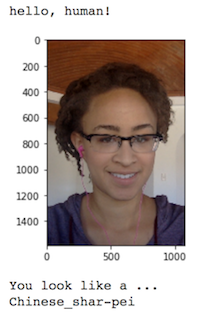
\includegraphics{images/sample_human_output.png}
\caption{Sample Human Output}
\end{figure}

\hypertarget{implementation-write-your-algorithm}{%
\subsubsection{(IMPLEMENTATION) Write your
Algorithm}\label{implementation-write-your-algorithm}}

    \begin{Verbatim}[commandchars=\\\{\}]
{\color{incolor}In [{\color{incolor}62}]:} \PY{k}{def} \PY{n+nf}{show\PYZus{}test\PYZus{}image}\PY{p}{(}\PY{n}{img\PYZus{}path}\PY{p}{)}\PY{p}{:}
             \PY{c+c1}{\PYZsh{} display the image}
             \PY{n}{img} \PY{o}{=} \PY{n}{cv2}\PY{o}{.}\PY{n}{imread}\PY{p}{(}\PY{n}{img\PYZus{}path}\PY{p}{)}
             \PY{n}{cv\PYZus{}rgb} \PY{o}{=} \PY{n}{cv2}\PY{o}{.}\PY{n}{cvtColor}\PY{p}{(}\PY{n}{img}\PY{p}{,} \PY{n}{cv2}\PY{o}{.}\PY{n}{COLOR\PYZus{}BGR2RGB}\PY{p}{)}
             \PY{n}{plt}\PY{o}{.}\PY{n}{imshow}\PY{p}{(}\PY{n}{cv\PYZus{}rgb}\PY{p}{)}
             \PY{n}{plt}\PY{o}{.}\PY{n}{show}\PY{p}{(}\PY{p}{)}
\end{Verbatim}


    \begin{Verbatim}[commandchars=\\\{\}]
{\color{incolor}In [{\color{incolor}63}]:} \PY{k}{def} \PY{n+nf}{predict\PYZus{}dog\PYZus{}model\PYZus{}transfer}\PY{p}{(}\PY{n}{img\PYZus{}path}\PY{p}{)}\PY{p}{:}
             \PY{n}{dog\PYZus{}prediction} \PY{o}{=} \PY{n}{model\PYZus{}transfer}\PY{p}{(}\PY{n}{image\PYZus{}preprocess}\PY{p}{(}\PY{n}{img\PYZus{}path}\PY{p}{)}\PY{p}{)}
             \PY{n}{dog\PYZus{}idx} \PY{o}{=} \PY{n+nb}{int}\PY{p}{(}\PY{n}{dog\PYZus{}prediction}\PY{o}{.}\PY{n}{argmax}\PY{p}{(}\PY{p}{)}\PY{o}{.}\PY{n}{cpu}\PY{p}{(}\PY{p}{)}\PY{o}{.}\PY{n}{numpy}\PY{p}{(}\PY{p}{)}\PY{p}{)}
             \PY{n}{dog\PYZus{}name} \PY{o}{=} \PY{n}{dog\PYZus{}classes}\PY{p}{[}\PY{n}{dog\PYZus{}idx}\PY{p}{]}\PY{o}{.}\PY{n}{split}\PY{p}{(}\PY{l+s+s1}{\PYZsq{}}\PY{l+s+s1}{.}\PY{l+s+s1}{\PYZsq{}}\PY{p}{)}\PY{p}{[}\PY{o}{\PYZhy{}}\PY{l+m+mi}{1}\PY{p}{]}
             \PY{k}{return} \PY{n}{dog\PYZus{}name}
         
         \PY{c+c1}{\PYZsh{} Simple test}
         \PY{c+c1}{\PYZsh{} img\PYZus{}path = dog\PYZus{}files\PYZus{}short[13]}
         \PY{c+c1}{\PYZsh{} predict\PYZus{}dog\PYZus{}model\PYZus{}transfer(img\PYZus{}path)}
\end{Verbatim}


    \begin{Verbatim}[commandchars=\\\{\}]
{\color{incolor}In [{\color{incolor}64}]:} \PY{k}{def} \PY{n+nf}{run\PYZus{}app}\PY{p}{(}\PY{n}{img\PYZus{}path}\PY{p}{)}\PY{p}{:}
             \PY{c+c1}{\PYZsh{}\PYZsh{} handle cases for a human face, dog, and neither}
             
             \PY{n}{show\PYZus{}test\PYZus{}image}\PY{p}{(}\PY{n}{img\PYZus{}path}\PY{p}{)}
             
             \PY{c+c1}{\PYZsh{} Detect human}
             \PY{k}{if} \PY{p}{(}\PY{n}{face\PYZus{}detector}\PY{p}{(}\PY{n}{img\PYZus{}path}\PY{p}{)}\PY{p}{)}\PY{p}{:}
                 \PY{n+nb}{print}\PY{p}{(}\PY{l+s+s2}{\PYZdq{}}\PY{l+s+s2}{Human detected. Human looks like dog breed ...}\PY{l+s+s2}{\PYZdq{}}\PY{p}{)}
                 \PY{n}{dog\PYZus{}breed} \PY{o}{=} \PY{n}{predict\PYZus{}breed\PYZus{}transfer}\PY{p}{(}\PY{n}{img\PYZus{}path}\PY{p}{)}
                 \PY{n+nb}{print}\PY{p}{(}\PY{n}{dog\PYZus{}breed}\PY{p}{)}
                 \PY{k}{return} \PY{n}{dog\PYZus{}breed}
             
             \PY{k}{if} \PY{p}{(}\PY{n}{dog\PYZus{}detector}\PY{p}{(}\PY{n}{img\PYZus{}path}\PY{p}{)}\PY{p}{)}\PY{p}{:}
                 \PY{n+nb}{print}\PY{p}{(}\PY{l+s+s2}{\PYZdq{}}\PY{l+s+s2}{Dog breed ...}\PY{l+s+s2}{\PYZdq{}}\PY{p}{)}
                 \PY{n}{dog\PYZus{}breed} \PY{o}{=} \PY{n}{predict\PYZus{}breed\PYZus{}transfer}\PY{p}{(}\PY{n}{img\PYZus{}path}\PY{p}{)}
                 \PY{n+nb}{print}\PY{p}{(}\PY{n}{dog\PYZus{}breed}\PY{p}{)}
                 \PY{k}{return} \PY{n}{dog\PYZus{}breed}
             
             \PY{n+nb}{print}\PY{p}{(}\PY{l+s+s2}{\PYZdq{}}\PY{l+s+s2}{Error: Neither dog nor human detected ...}\PY{l+s+s2}{\PYZdq{}}\PY{p}{)}
             \PY{k}{return} \PY{k+kc}{None}
\end{Verbatim}


    \begin{center}\rule{0.5\linewidth}{\linethickness}\end{center}

 \#\# Step 6: Test Your Algorithm

In this section, you will take your new algorithm for a spin! What kind
of dog does the algorithm think that \emph{you} look like? If you have a
dog, does it predict your dog's breed accurately? If you have a cat,
does it mistakenly think that your cat is a dog?

\hypertarget{implementation-test-your-algorithm-on-sample-images}{%
\subsubsection{(IMPLEMENTATION) Test Your Algorithm on Sample
Images!}\label{implementation-test-your-algorithm-on-sample-images}}

Test your algorithm at least six images on your computer. Feel free to
use any images you like. Use at least two human and two dog images.

\textbf{Question 6:} Is the output better than you expected :) ? Or
worse :( ? Provide at least three possible points of improvement for
your algorithm.

    \textbf{Answer:}

The output is better than I expected for the dog classifications. It is
a bit hard to measure the closest dog breed match to the human face.
Some improvements to the algorithm are.

\begin{enumerate}
\def\labelenumi{\arabic{enumi}.}
\tightlist
\item
  The algorithm has some challenges when there are multiple humans in
  the photo. We could improve accuracy of the current face detector by
  building a deep network for human faces.
\item
  There is no easy way to validate how good our classification scheme
  does in detecting the closest dog breed to a human face. We can
  collect some label data (by asking users) on whether the prediction
  was approved by humans by juxtaposing a representative image of a dog
  next to the human. With those lables, we can train a network to do the
  closest-human-dog match.
\item
  The top 5 misclassification among dog breeds is as follows: (`Kuvasz',
  `English\_cocker\_spaniel', `Silky\_terrier', `Doberman\_pinscher',
  `Lakeland\_terrier'). In order to bring down the misclassification
  rate, we can collect more images on these dogs that are being
  misclassified for better discrimination.
\end{enumerate}

    \begin{Verbatim}[commandchars=\\\{\}]
{\color{incolor}In [{\color{incolor}65}]:} \PY{c+c1}{\PYZsh{} Set to true to see true class labels of predictions.}
         \PY{n}{debug\PYZus{}app} \PY{o}{=} \PY{k+kc}{False}
\end{Verbatim}


    \begin{Verbatim}[commandchars=\\\{\}]
{\color{incolor}In [{\color{incolor}66}]:} \PY{k+kn}{from} \PY{n+nn}{random} \PY{k}{import} \PY{n}{randint}
         \PY{n}{num\PYZus{}test\PYZus{}points} \PY{o}{=} \PY{l+m+mi}{10}
         \PY{n}{img\PYZus{}idx} \PY{o}{=} \PY{p}{[}\PY{n}{randint}\PY{p}{(}\PY{l+m+mi}{0}\PY{p}{,} \PY{l+m+mi}{8000}\PY{p}{)} \PY{k}{for} \PY{n}{i} \PY{o+ow}{in} \PY{n+nb}{range}\PY{p}{(}\PY{l+m+mi}{0}\PY{p}{,} \PY{n}{num\PYZus{}test\PYZus{}points} \PY{o}{\PYZhy{}} \PY{l+m+mi}{1}\PY{p}{)}\PY{p}{]}
         \PY{n}{img\PYZus{}idx}
         
         \PY{n}{fn\PYZus{}path\PYZus{}to\PYZus{}name} \PY{o}{=} \PY{k}{lambda} \PY{n}{x}\PY{p}{:} \PY{n}{os}\PY{o}{.}\PY{n}{path}\PY{o}{.}\PY{n}{split}\PY{p}{(}\PY{n}{file}\PY{p}{)}\PY{p}{[}\PY{o}{\PYZhy{}}\PY{l+m+mi}{1}\PY{p}{]}\PY{o}{.}\PY{n}{split}\PY{p}{(}\PY{l+s+s1}{\PYZsq{}}\PY{l+s+s1}{.}\PY{l+s+s1}{\PYZsq{}}\PY{p}{)}\PY{p}{[}\PY{l+m+mi}{0}\PY{p}{]}
         
         \PY{k}{for} \PY{n}{file} \PY{o+ow}{in} \PY{n}{np}\PY{o}{.}\PY{n}{hstack}\PY{p}{(}\PY{p}{(}\PY{n}{human\PYZus{}files}\PY{p}{[}\PY{n}{img\PYZus{}idx}\PY{p}{]}\PY{p}{,} \PY{n}{dog\PYZus{}files}\PY{p}{[}\PY{n}{img\PYZus{}idx}\PY{p}{]}\PY{p}{)}\PY{p}{)}\PY{p}{:}
             \PY{n}{dog\PYZus{}breed} \PY{o}{=} \PY{n}{run\PYZus{}app}\PY{p}{(}\PY{n}{file}\PY{p}{)}
             
             \PY{k}{if} \PY{p}{(}\PY{n}{debug\PYZus{}app}\PY{p}{)}\PY{p}{:}
                 \PY{n+nb}{print}\PY{p}{(}\PY{l+s+s2}{\PYZdq{}}\PY{l+s+s2}{True class name: }\PY{l+s+si}{\PYZob{}0\PYZcb{}}\PY{l+s+s2}{\PYZdq{}}\PY{o}{.}\PY{n}{format}\PY{p}{(}\PY{n}{fn\PYZus{}path\PYZus{}to\PYZus{}name}\PY{p}{(}\PY{n}{file}\PY{p}{)}\PY{p}{)}\PY{p}{)}
\end{Verbatim}


    \begin{center}
    \adjustimage{max size={0.9\linewidth}{0.9\paperheight}}{output_66_0.png}
    \end{center}
    { \hspace*{\fill} \\}
    
    \begin{Verbatim}[commandchars=\\\{\}]
Human detected. Human looks like dog breed {\ldots}
Dogue\_de\_bordeaux

    \end{Verbatim}

    \begin{center}
    \adjustimage{max size={0.9\linewidth}{0.9\paperheight}}{output_66_2.png}
    \end{center}
    { \hspace*{\fill} \\}
    
    \begin{Verbatim}[commandchars=\\\{\}]
Human detected. Human looks like dog breed {\ldots}
Dogue\_de\_bordeaux

    \end{Verbatim}

    \begin{center}
    \adjustimage{max size={0.9\linewidth}{0.9\paperheight}}{output_66_4.png}
    \end{center}
    { \hspace*{\fill} \\}
    
    \begin{Verbatim}[commandchars=\\\{\}]
Human detected. Human looks like dog breed {\ldots}
Dogue\_de\_bordeaux

    \end{Verbatim}

    \begin{center}
    \adjustimage{max size={0.9\linewidth}{0.9\paperheight}}{output_66_6.png}
    \end{center}
    { \hspace*{\fill} \\}
    
    \begin{Verbatim}[commandchars=\\\{\}]
Human detected. Human looks like dog breed {\ldots}
Dogue\_de\_bordeaux

    \end{Verbatim}

    \begin{center}
    \adjustimage{max size={0.9\linewidth}{0.9\paperheight}}{output_66_8.png}
    \end{center}
    { \hspace*{\fill} \\}
    
    \begin{Verbatim}[commandchars=\\\{\}]
Human detected. Human looks like dog breed {\ldots}
Irish\_water\_spaniel

    \end{Verbatim}

    \begin{center}
    \adjustimage{max size={0.9\linewidth}{0.9\paperheight}}{output_66_10.png}
    \end{center}
    { \hspace*{\fill} \\}
    
    \begin{Verbatim}[commandchars=\\\{\}]
Human detected. Human looks like dog breed {\ldots}
Dogue\_de\_bordeaux

    \end{Verbatim}

    \begin{center}
    \adjustimage{max size={0.9\linewidth}{0.9\paperheight}}{output_66_12.png}
    \end{center}
    { \hspace*{\fill} \\}
    
    \begin{Verbatim}[commandchars=\\\{\}]
Human detected. Human looks like dog breed {\ldots}
Otterhound

    \end{Verbatim}

    \begin{center}
    \adjustimage{max size={0.9\linewidth}{0.9\paperheight}}{output_66_14.png}
    \end{center}
    { \hspace*{\fill} \\}
    
    \begin{Verbatim}[commandchars=\\\{\}]
Human detected. Human looks like dog breed {\ldots}
Afghan\_hound

    \end{Verbatim}

    \begin{center}
    \adjustimage{max size={0.9\linewidth}{0.9\paperheight}}{output_66_16.png}
    \end{center}
    { \hspace*{\fill} \\}
    
    \begin{Verbatim}[commandchars=\\\{\}]
Human detected. Human looks like dog breed {\ldots}
Bearded\_collie

    \end{Verbatim}

    \begin{center}
    \adjustimage{max size={0.9\linewidth}{0.9\paperheight}}{output_66_18.png}
    \end{center}
    { \hspace*{\fill} \\}
    
    \begin{Verbatim}[commandchars=\\\{\}]
Dog breed {\ldots}
American\_staffordshire\_terrier

    \end{Verbatim}

    \begin{center}
    \adjustimage{max size={0.9\linewidth}{0.9\paperheight}}{output_66_20.png}
    \end{center}
    { \hspace*{\fill} \\}
    
    \begin{Verbatim}[commandchars=\\\{\}]
Human detected. Human looks like dog breed {\ldots}
Bullmastiff

    \end{Verbatim}

    \begin{center}
    \adjustimage{max size={0.9\linewidth}{0.9\paperheight}}{output_66_22.png}
    \end{center}
    { \hspace*{\fill} \\}
    
    \begin{Verbatim}[commandchars=\\\{\}]
Dog breed {\ldots}
Wirehaired\_pointing\_griffon

    \end{Verbatim}

    \begin{center}
    \adjustimage{max size={0.9\linewidth}{0.9\paperheight}}{output_66_24.png}
    \end{center}
    { \hspace*{\fill} \\}
    
    \begin{Verbatim}[commandchars=\\\{\}]
Dog breed {\ldots}
Bearded\_collie

    \end{Verbatim}

    \begin{center}
    \adjustimage{max size={0.9\linewidth}{0.9\paperheight}}{output_66_26.png}
    \end{center}
    { \hspace*{\fill} \\}
    
    \begin{Verbatim}[commandchars=\\\{\}]
Dog breed {\ldots}
Dogue\_de\_bordeaux

    \end{Verbatim}

    \begin{center}
    \adjustimage{max size={0.9\linewidth}{0.9\paperheight}}{output_66_28.png}
    \end{center}
    { \hspace*{\fill} \\}
    
    \begin{Verbatim}[commandchars=\\\{\}]
Dog breed {\ldots}
Neapolitan\_mastiff

    \end{Verbatim}

    \begin{center}
    \adjustimage{max size={0.9\linewidth}{0.9\paperheight}}{output_66_30.png}
    \end{center}
    { \hspace*{\fill} \\}
    
    \begin{Verbatim}[commandchars=\\\{\}]
Human detected. Human looks like dog breed {\ldots}
Gordon\_setter

    \end{Verbatim}

    \begin{center}
    \adjustimage{max size={0.9\linewidth}{0.9\paperheight}}{output_66_32.png}
    \end{center}
    { \hspace*{\fill} \\}
    
    \begin{Verbatim}[commandchars=\\\{\}]
Dog breed {\ldots}
Boykin\_spaniel

    \end{Verbatim}

    \begin{center}
    \adjustimage{max size={0.9\linewidth}{0.9\paperheight}}{output_66_34.png}
    \end{center}
    { \hspace*{\fill} \\}
    
    \begin{Verbatim}[commandchars=\\\{\}]
Dog breed {\ldots}
Irish\_wolfhound

    \end{Verbatim}


    % Add a bibliography block to the postdoc
    
    
    
    \end{document}
